\documentclass[a4paper]{article}
\usepackage[T1]{fontenc}			% \chapter package
\usepackage[english]{babel}
\usepackage[english]{isodate}  		% date format
\usepackage{graphicx}				% manage images
\usepackage{amsfonts}
\usepackage{booktabs}				% high quality tables
\usepackage{amsmath}				% math package
\usepackage{amssymb}				% another math package (e.g. \nexists)
\usepackage{bm}                     % bold math symbols
\usepackage{mathtools}				% emphasize equations
\usepackage{stmaryrd} 				% '\llbracket' and '\rrbracket'
\usepackage{amsthm}					% better theorems
\usepackage{enumitem}				% manage list
\usepackage{pifont}					% nice itemize
\usepackage{cancel}					% cancel math equations
\usepackage{caption}				% custom caption
\usepackage[]{mdframed}				% box text
\usepackage{multirow}				% more lines in a table
\usepackage{textcomp, gensymb}		% degree symbol
\usepackage[x11names]{xcolor}		% RGB color
\usepackage[many]{tcolorbox}				% colorful box
\usepackage{multicol}				% more rows in a table (used for the lists)
\usepackage{listings}
\usepackage{url}
\usepackage{qrcode}
\usepackage{fontawesome5}
\usepackage{ragged2e}
\usepackage{cite}                   % references
\usepackage{imakeidx}               % index
\makeindex[program=makeindex, columns=2,
           title=Index, 
           intoc,
           options={-s index-style.ist}]


\definecolor{codegreen}{rgb}{0,0.6,0}
\definecolor{codegray}{rgb}{0.5,0.5,0.5}
\definecolor{codepurple}{rgb}{0.58,0,0.82}
\definecolor{backcolour}{rgb}{0.95,0.95,0.92}
\lstdefinestyle{mystyle}{
    backgroundcolor=\color{backcolour},   
    commentstyle=\color{codegreen},
    keywordstyle=\color{magenta},
    numberstyle=\tiny\color{codegray},
    stringstyle=\color{codepurple},
    basicstyle=\ttfamily\footnotesize,
    breakatwhitespace=false,         
    breaklines=true,                 
    captionpos=b,                    
    keepspaces=true,                 
    numbers=left,                    
    numbersep=5pt,                  
    showspaces=false,                
    showstringspaces=false,
    showtabs=false,                  
    tabsize=2
}
\lstset{
  language=R,
  basicstyle=\footnotesize\ttfamily,
  literate=~{$\sim$}2
}
\lstset{style=mystyle}


% draw a frame around given text
\newcommand{\framedtext}[1]{%
	\par%
	\noindent\fbox{%
		\parbox{\dimexpr\linewidth-2\fboxsep-2\fboxrule}{#1}%
	}%
}


% table of content links
\usepackage{xcolor}
\usepackage[linkcolor=black, citecolor=blue, urlcolor=cyan]{hyperref} % hypertexnames=false
\hypersetup{
	colorlinks=true
}


\newtheorem{theorem}{\textcolor{Red3}{\underline{Theorem}}}
\renewcommand{\qedsymbol}{QED}
\newcommand{\dquotes}[1]{``#1''}
\newcommand{\longline}{\noindent\rule{\textwidth}{0.4pt}}
\newcommand{\circledtext}[1]{\raisebox{.5pt}{\textcircled{\raisebox{-.9pt}{#1}}}}
\newcommand{\definition}[1]{\textcolor{Red3}{\textbf{#1}}\index{#1}}
\newcommand{\example}[1]{\textcolor{Green4}{\textbf{#1}}}
\newcommand{\Var}{\mathrm{Var}}
\newcommand{\Bias}{\mathrm{Bias}}
\newcommand{\Cov}{\mathrm{Cov}}
\newcommand{\highspace}{\vspace{1.2em}\noindent}
\newcommand{\tr}{\mathrm{tr}}
\newenvironment{rowequmat}[1]{\left(\array{@{}#1@{}}}{\endarray\right)}
\newenvironment{rowequmatbra}[1]{\left[\array{@{}#1@{}}}{\endarray\right]}


\begin{document}
    \newcounter{definition}[section]
    \newcounter{example}[section]
    
    \newtcolorbox[use counter = definition]{definitionbox}{%
        colback=red!5!white,
        colframe=red!75!black,
        fonttitle=\bfseries,
        title=Definition \thetcbcounter %
    }
    
    \newtcolorbox[use counter = example]{examplebox}{%
        breakable,
        enhanced,
        colback=Green4!5!white,
        colframe=Green4!75!black,
        fonttitle=\bfseries,
        title=Example \thetcbcounter %
    }

    \author{260236}
	\title{Applied Statistics - Notes}
	\date{\printdayoff\today}
	\maketitle

	\newpage

    \section*{Preface}

    Every theory section in these notes has been taken from two sources:
    \begin{itemize}
        \item \href{https://www.statlearning.com/}{An Introduction to Statistical Learning}\cite{james2013introduction}
        \item Applied Multivariate Statistical Analysis (sixth edition).\cite{johnson2007applied}
    \end{itemize}
    About:
    \begin{itemize}
        \item[\faIcon{github}] \href{https://github.com/AndreVale69/HPC-E-PoliMI-university-notes}{GitHub repository}
    \end{itemize}
    
    \newpage
	
	\tableofcontents
	
	\newpage

    \section{Sample Geometry}

    \subsection{The Geometry of the Sample}

    \underline{A single} \definition{multivariate observation} is the \textbf{collection of measurements on $p$ different variables taken on the same item or trial}. If \textbf{$n$ observations} have been obtained, the entire data set can be placed in an $n \times p$ array (or matrix), also called \definition{data frame}:
    \begin{equation}\label{eq: data frame matrix}
        \underset{\left(n \times p\right)}{\mathbf{X}} = \begin{bmatrix}
            x_{11} & x_{12} & \cdots & x_{1p} \\
            x_{21} & x_{22} & \cdots & x_{2p} \\
            \vdots & \vdots & \ddots & \vdots \\
            x_{n1} & x_{n2} & \cdots & x_{np}
        \end{bmatrix}
    \end{equation}
    Each \textbf{row} of $\mathbf{X}$ represents a \textbf{multivariate observation}. Since the entire data frame is often one particular realization of what might have been observed, we say that the data frame are a \textbf{sample of size $n$ from a $p$-variate \dquotes{population}}. The sample then consists of $n$ measurements, each of which has $p$ components.

    Look at the matrix, $n$ measurements (rows), each of which has $p$ components (columns). In mathematics, each $n$ row contains $p$ columns and vice versa.
    
    \highspace
    The data frame can be plotted in two different ways:
    \begin{enumerate}
        \item $p$-dimensional scatter plot, where the rows represent $n$ points in \emph{p}-dimensional space;
        \item Geometrical representation, $p$ vectors in $n$-dimensional space.
    \end{enumerate}
    
    \longline

    \subsubsection{Scatter plot}

    For the \definition{$p$-dimensional scatter plot}, the rows of $\mathbf{X}$ represent $n$ points in $p$-dimensional space:
    \begin{equation}\label{eq: p-dimensional scatter plot}
        \underset{\left(n \times p\right)}{\mathbf{X}} = \begin{bmatrix}
            x_{11} & x_{12} & \cdots & x_{1p} \\
            x_{21} & x_{22} & \cdots & x_{2p} \\
            \vdots & \vdots & \ddots & \vdots \\
            x_{n1} & x_{n2} & \cdots & x_{np}
        \end{bmatrix} = \left[\begin{array}{@{} c @{}}
            \mathbf{x}_{1}' \\
            \mathbf{x}_{2}' \\
            \vdots \\
            \mathbf{x}_{n}'
        \end{array}\right]
        \begin{array}{l}
            \leftarrow \text{1st (multivariate) observation} \\
            \phantom{\mathbf{x}_{2}'} \\
            \phantom{\vdots} \\
            \leftarrow n\text{th (multivariate) observation}
        \end{array}
    \end{equation}
    The row vector $\mathbf{x}_{j}'$, representing the $j$th observation, contains the coordinates of a point. The \textbf{scatter plot} of $n$ points in $p$-dimensional space \textbf{provides information} on the \textbf{locations and variability of the points}.
    
    \highspace
    \underline{\textbf{Note}}: when $p$ (dimensional space) is greater than $3$, the \textbf{scatter plot} representation cannot actually be graphed. Yet the consideration of the data as $n$ points in $p$ dimensions provides \textbf{insights that are not readily available from algebraic expressions}.

    \newpage

    \subsubsection{Geometrical representation}

    The alternative \definition{geometrical representation} is constructed by considering the data as \textbf{$p$ vectors in $n$-dimensional space}. Here we take the elements of the columns of the data frame to be the coordinates of the vectors:
    \begin{equation}\label{eq: geometrical representation}
        \underset{\left(n \times p\right)}{\mathbf{X}} = \begin{bmatrix}
            x_{11} & x_{12} & \cdots & x_{1p} \\
            x_{21} & x_{22} & \cdots & x_{2p} \\
            \vdots & \vdots & \ddots & \vdots \\
            x_{n1} & x_{n2} & \cdots & x_{np}
        \end{bmatrix} = \left[\mathbf{y}_{1} \: | \: \mathbf{y}_{2} \: | \: \cdots \: | \: \mathbf{y}_{p}\right]
    \end{equation}
    Then the \textbf{coordinates} of the first point $\mathbf{y}_{1} = \left[x_{11}, x_{21}, \dots, x_{n1}\right]$ \textbf{are the $n$ measurements} on the first variable. 
    
    In general, the $i$th point $\mathbf{y}_{i} = \left[x_{11}, x_{21}, \dots, x_{n1}\right]$ is determined by the $n$-tuple of all measurements on the $i$th variable.
    
    \highspace
    \textbf{Geometrical representations} usually \textbf{facilitate understanding} and lead to further insights. The ability to \textbf{relate algebraic expressions to the geometric concepts} of length, angle and volume is therefore \textbf{very important}.
    
    \highspace
    \longline

    \subsubsection{Geometrical interpretation of the process of finding a sample mean}

    Before starting the explanation, you need to understand a few things.
    \begin{itemize}
        \item The \definition{length} of a vector $\mathbf{x}'=\left[x_{1}, x_{2}, \dots, x_{n}\right]$ with $n$ components is defined by:
        \begin{equation}\label{eq: length of a vector}
            L_{x} = \sqrt{x_{1}^{2} + x_{2}^{2} + \cdots + x_{n}^{2}}
        \end{equation}
        Multiplication of a vector $\mathbf{x}$ by a scalar $c$ changes the length:
        \begin{equation*}
            \begin{array}{rcl}
                L_{cx} &=& \sqrt{c^{2} \cdot x_{1}^{2} + c^{2} \cdot x_{2}^{2} + \cdots + c^{2} \cdot x_{n}^{2}} \\ [.3em]
                %
                &=& \left| c \right| \sqrt{x_{1}^{2} + x_{2}^{2} + \cdots + x_{n}^{2}} \\ [.3em] 
                %
                &=& \left| c \right| L_{x}
            \end{array}
        \end{equation*}
        So, for example, in $n = 2$ dimensions, the vector:
        \begin{equation*}
            \mathbf{x} = \begin{bmatrix}
                x_{1} \\ x_{2}
            \end{bmatrix}
        \end{equation*}
        The length of $\mathbf{x}$, written $L_{x}$, is defined to be:
        \begin{equation*}
            L_{x} = \sqrt{x_{1}^{2} + x_{2}^{2}}
        \end{equation*}

        \newpage

        \item Another important concept is \definition{angle}. Consider two vectors in a plane and the angle $\theta$ between them:
        \begin{figure}[!htp]
            \centering
            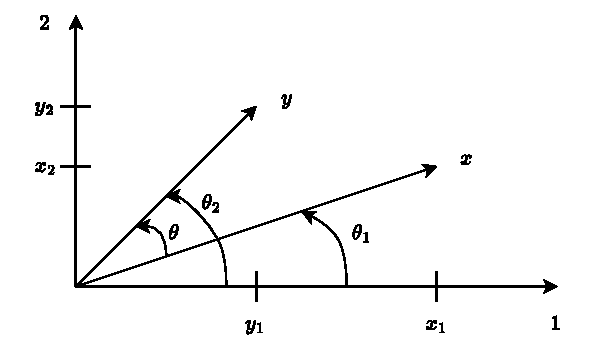
\includegraphics[width=.7\textwidth]{img/basics-vector-algebra-1.pdf}
            \caption{The angle $\theta$ between $\mathbf{x}' = \left[x_{1}, x_{2}\right]$ and $\mathbf{y}' = \left[y_{1}, y_{2}\right]$.}
        \end{figure}
        The value $\theta$ can be represented as the difference between the angles $\theta_{1}$ and $\theta_{2}$ formed by the two vectors and the first coordinate axis. Since, by definition:
        \begin{gather*}
            \begin{array}{rcl}
                \cos\left(\theta_{1}\right) = \dfrac{x_{1}}{L_{x}} & \cos\left(\theta_{2}\right) = \dfrac{y_{1}}{L_{y}} \\ [1em]
                %
                \sin\left(\theta_{1}\right) = \dfrac{x_{2}}{L_{x}} & \sin\left(\theta_{2}\right) = \dfrac{y_{2}}{L_{y}}
            \end{array} \\
            \cos\left(\theta\right) = \cos\left(\theta_{2} - \theta_{1}\right) = \cos\left(\theta_{2}\right) \cos\left(\theta_{1}\right) + \sin\left(\theta_{2}\right) \sin\left(\theta_{1}\right)
        \end{gather*}
        The angle $\theta$ between the two vectors $\mathbf{x}' = \left[x_{1}, x_{2}\right]$ and $\mathbf{y}' = \left[y_{1}, y_{2}\right]$ is specified by:
        \begin{equation}\label{eq: angle}
            \cos\left(\theta\right) = \cos\left(\theta_{2} - \theta_{1}\right) = 
            \left(\dfrac{y_{1}}{L_{y}}\right)\left(\dfrac{x_{1}}{L_{x}}\right) + \left(\dfrac{y_{2}}{L_{y}}\right)\left(\dfrac{x^{2}}{L_{x}}\right) =
            \dfrac{x_{1}y_{1} + x_{2}y_{2}}{L_{x}L_{y}}
        \end{equation}

        \item With the angle equation~\ref{eq: angle}, it's convenient to introduce the \definition{inner product} of two vectors:
        \begin{equation*}
            \mathbf{x}\mathbf{y}' = x_{1}y_{1} + x_{2}y_{2}
        \end{equation*}
        So let us rewrite:
        \begin{itemize}
            \item The \textbf{length} equation~\ref{eq: length of a vector}:
            \begin{equation}\label{eq: length rewritten with inner product}
                \mathbf{x}'\mathbf{x} = x_{1} x_{1} + x_{1} x_{1} = x_{1}^{2} + x_{2}^{2} 
                \longrightarrow
                L_{x} = \sqrt{x_{1}^{2} + x_{2}^{2}}
                \Longrightarrow
                L_{x} = \sqrt{\mathbf{x}' \mathbf{x}}
            \end{equation}

            \item The \textbf{angle} equation~\ref{eq: angle}:
            \begin{equation*}
                \cos\left(\theta\right) = \dfrac{x_{1}y_{1} + x_{2}y_{2}}{L_{x}L_{y}} 
                \Longrightarrow
                \cos\left(\theta\right) = \dfrac{\mathbf{x}'\mathbf{y}}{L_{x}L_{y}}
            \end{equation*}
            And using the rewritten length equation:
            \begin{equation*}
                \cos\left(\theta\right) = \dfrac{\mathbf{x}'\mathbf{y}}{L_{x}L_{y}} \Longrightarrow
                \cos\left(\theta\right) = \dfrac{\mathbf{x}'\mathbf{y}}{\sqrt{\mathbf{x}' \mathbf{x}} \cdot \sqrt{\mathbf{y}' \mathbf{y}}}
            \end{equation*}
        \end{itemize}
        
        \item The \definition{projection} (or shadow) of a vector $\mathbf{x}$ on a vector $\mathbf{y}$ is:
        \begin{equation}\label{eq: projection}
            \dfrac{\left(\mathbf{x}'\mathbf{y}\right)}{\mathbf{y}'\mathbf{y}}\mathbf{y} = \dfrac{\left(\mathbf{x}'\mathbf{y}\right)}{L_{y}}\dfrac{1}{L_{y}}\mathbf{y}
        \end{equation}
        Where the vector $\dfrac{1}{L_{y}}\mathbf{y}$ has unit length. The \textbf{length of the projection} is:
        \begin{equation}\label{eq: length of the projection}
            \dfrac{\left| \mathbf{x}'\mathbf{y} \right|}{L_{y}} = L_{x} \left| \dfrac{\mathbf{x}'\mathbf{y}}{L_{x}L_{y}} \right| = L_{x} \left| \cos\left(\theta\right) \right|
        \end{equation}
        Where $\theta$ is the angle between $\mathbf{x}$ and $\mathbf{y}$:
        \begin{figure}[!htp]
            \centering
            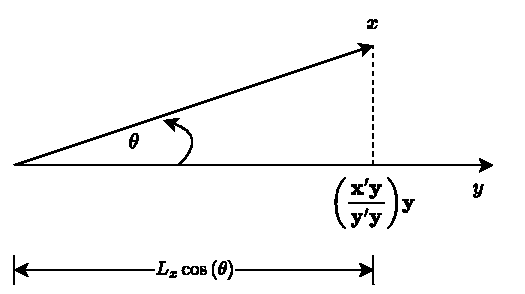
\includegraphics[width=.7\textwidth]{img/basics-vector-algebra-2.pdf}
            \caption{The projection of $\mathbf{x}$ on $\mathbf{y}$.}
        \end{figure}
    \end{itemize}
    Start by defining the $n \times 1$ vector $\mathbf{1}_{n}' = \left[1, 1, \dots, 1\right]$. The vector $\mathbf{1}$ forms equal angles with each of the $n$ coordinates axes, so the vector $\left(\dfrac{1}{\sqrt{n}}\right)\mathbf{1}$ has unit length in the equal-angle direction. Consider the vector $\mathbf{y}_{i}' = \left[x_{1i}, x_{2i}, \dots, x_{ni}\right]$. The projection of $\mathbf{y}_{i}$ on the unit vector $\left(\dfrac{1}{\sqrt{n}}\right)\mathbf{1}$ is:
    \begin{equation}\label{eq: sample mean - geometrical representation}
        \mathbf{y}_{i}'\left(\dfrac{1}{\sqrt{n}}\mathbf{1}\right)\dfrac{1}{\sqrt{n}}\mathbf{1} = 
        \dfrac{x_{1i} + x_{2i} + \cdots + x_{ni}}{n}\mathbf{1} = \overline{x}_{i}\mathbf{1}
    \end{equation}
    Although it may seem like a complex equation at first glance, it is nothing more than the mean! In fact, the \textbf{sample mean} $\overline{\mathbf{x}}_{i} = \dfrac{\left(x_{1i} + x_{2i} + \cdots + x_{ni}\right)}{n} = \dfrac{\mathbf{y}_{i}' \mathbf{1}}{n}$ corresponds to the multiple of $\mathbf{1}$ required to give the projection of $\mathbf{y}_{i}$ onto the line determined by $\mathbf{1}$.\newpage

    \noindent
    Furthermore, using the projection, you can obtain the \textbf{deviation} (\textbf{mean corrected}). For each $\mathbf{y}_{i}$ we have the decomposition:
    \begin{figure}[!htp]
        \centering
        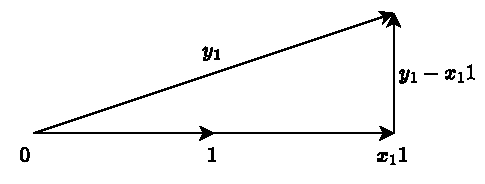
\includegraphics[width=.6\textwidth]{img/basics-vector-algebra-3.pdf}
    \end{figure}

    \noindent
    Where $\overline{x}_{i} \mathbf{1}$ is perpendicular to $y_{i}-\overline{x}_{i}\mathbf{1}$. The \definition{deviation}, or \definition{mean corrected}, vector is:
    \begin{equation}\label{eq: deviation - mean corrected}
        \mathbf{d}_{i} = \mathbf{y}_{i} - \overline{x}_{i}\mathbf{1} = \begin{bmatrix}
            x_{1i} - \overline{x}_{i} \\
            x_{2i} - \overline{x}_{i} \\
            \vdots \\
            x_{ni} - \overline{x}_{i}
        \end{bmatrix}
    \end{equation}
    The \textbf{elements} of $\mathbf{d}_{i}$ are the \textbf{deviations of the measurements on the} $\bm{i}$\textbf{th variable from their sample mean}.\newline

    \noindent
    Using the length rewritten with inner product (equation~\ref{eq: length rewritten with inner product}) and the deviation (equation~\ref{eq: deviation - mean corrected}), we obtain:
    \begin{equation}
        L_{\mathbf{d}_{i}}^{2} = \mathbf{d}_{i}'\mathbf{d}_{i} = \displaystyle\sum_{j=1}^{n}\left(x_{ji}-\overline{x}_{i}\right)^{2}
    \end{equation}
    \begin{equation*}
        \left(\text{Length of deviation vector}\right)^{2} = \text{sum of squared deviations}
    \end{equation*}
    From the sample standard deviation, we see that the \textbf{squared length is proportional to the variance} of the measurements on the $i$th variable. Equivalently, the \textbf{length is proportional to the standard deviation}. So longer vectors represent more variability than shorter vectors.

    Furthermore, for any two deviation vectors $\mathbf{d}_{i}$ and $\mathbf{d}_{k}$:
    \begin{equation}
        \mathbf{d}_{i}'\mathbf{d}_{k} = \displaystyle\sum_{j=1}^{n}\left(x_{ji} - \overline{x}_{i}\right)\left(x_{jk} - \overline{x}_{k}\right)
    \end{equation}
    And with a few mathematical operations, we can get it:
    \begin{equation}
        r_{ik} = \dfrac{s_{ik}}{\sqrt{s_{ii}}\sqrt{s_{kk}}} = \cos\left(\theta_{ik}\right)
    \end{equation}
    Where the \textbf{cosine} of the angle is the \definition{sample correlation coefficient}. Note: $s_{ik}$ is the \definition{sample covariance}:
    \begin{equation}\label{eq: sample covariance}
        s_{ik} = \dfrac{1}{n} \displaystyle\sum_{j=1}^{n} \left(x_{ji} - \overline{x}_{i}\right)\left(x_{jk} - \overline{x}_{k}\right) \hspace{2em} i = 1,2,\dots,p, \hspace{1em} k = 1,2,\dots,p
    \end{equation}
    Thus:
    \begin{itemize}
        \item If the two deviation vectors have \textbf{nearly the same orientation}, the sample correlation will be close to $1$;
        \item If the two vectors are \textbf{nearly perpendicular}, the sample correlation will be approximately zero;
        \item If the two vectors are oriented in \textbf{nearly opposite directions}, the sample correlation will be close to $-1$.
    \end{itemize}

    \longline

    \subsection{Generalized Variance}

    Before starting the explanation, you need to understand what is a sample variance.

    A \definition{sample variance} is defined as:
    \begin{equation}\label{eq: sample variance}
        s_{k}^{2} = s_{kk} = \dfrac{1}{n-1} \displaystyle\sum_{j=1}^{n} \left(x_{jk} - \overline{x}_{k}\right)^{2} \hspace{2em} k = 1, 2, \dots, p
    \end{equation}

    With a single variable, the \textbf{sample variance is often used to describe the amount of variation in the measurements on that variable}. When $p$ variables are observed on each unit, the variation is described by the \definition{sample variance-covariance matrix}:
    \begin{equation}
        \mathbf{S} = \begin{bmatrix}
            s_{11} & s_{12} & \cdots & s_{1p} \\
            s_{21} & s_{22} & \cdots & s_{2p} \\
            \vdots & \vdots & \ddots & \vdots \\
            s_{p1} & s_{p2} & \cdots & s_{pp}
        \end{bmatrix} =
        \left\{s_{ik} = \dfrac{1}{n-1}\displaystyle\sum_{j=1}^{n}\left(x_{ji}-\overline{x}_{i}\right)\left(x_{jk}-\overline{x}_{k}\right)\right\}
    \end{equation}
    The sample covariance matrix contains $p$ variances and $\dfrac{1}{2}p\left(p-1\right)$ potentially different covariances. Sometimes it's desirable to \textbf{assign a single numerical value for the variation expressed by $\mathbf{S}$}. One choice for a value is the \href{https://en.wikipedia.org/wiki/Determinant}{determinant} of $\mathbf{S}$, which reduces to the usual sample variance of a single characteristic when $p=1$. This determinant is called the \definition{generalized sample variance}:
    \begin{equation}
        \text{Generalized sample variance} = \det\left(\mathbf{S}\right) = \left| \mathbf{S} \right|
    \end{equation}
    \underline{Note} that the determinant of $\mathbf{S}$ $\det\left(\mathbf{S}\right)$ is zero if and only if the deviation vectors are linearly dependent:
    \begin{equation}
        \det\left(\mathbf{S}\right) = 0 \iff \mathbf{d}_{1}, \dots, \mathbf{d}_{p} \text{ are linearly dependent}
    \end{equation}
    Another value used, but not often as a determinant, is the trace\footnote{In linear algebra, the trace of a square matrix $A$, denoted $\tr(A)$, is defined to be the sum of elements on the main diagonal (from the upper left to the lower right) of $A$. The trace is only defined for a square matrix ($n \times n$).}. With this operation we can obtain the \definition{total variance}:
    \begin{equation}
        \text{Total variance } = \tr\left(\mathbf{S}\right) = s_{11} + s_{22} + \cdots + s_{pp}
    \end{equation}
    
    \newpage

    \subsection{Random Vectors and Matrices}

    A \definition{random vector} is a \textbf{vector whose elements are random variables}. Similarly, a \definition{random matrix} is a \textbf{matrix whose elements are random variables}.

    \highspace
    The expected value of a random matrix (or vector) is the matrix (vector) consisting of the \textbf{expected values of each of its elements}.

    \highspace
    Let $\mathbf{X} = \left\{X_{ij}\right\}$ be an $n \times p$ random matrix. Then the expected value of $\mathbf{X}$, denoted by $E\left(\mathbf{X}\right)$, is the $n \times p$ matrix of numbers (if they exist):
    \begin{equation}\label{eq: random vectors and matrices}
        E\left(\mathbf{X}\right) = \begin{bmatrix}
            E\left(X_{11}\right) & E\left(X_{12}\right) & \cdots & E\left(X_{1p}\right) \\ 
            E\left(X_{21}\right) & E\left(X_{22}\right) & \cdots & E\left(X_{2p}\right) \\ 
            \vdots               & \vdots               & \ddots & \vdots               \\ 
            E\left(X_{n1}\right) & E\left(X_{n2}\right) & \cdots & E\left(X_{np}\right)
        \end{bmatrix}
    \end{equation}
    Where, for each element of the matrix:
    \begin{equation*}
        E\left(X_{ij}\right) = \begin{cases}
            \displaystyle \int_{-\infty}^{\infty} x_{ij} \: f_{ij}\left(x_{ij}\right) \:\mathrm{d}x_{ij} & \text{if }X_{ij}\text{ is a continuous random variable} \vspace{-.5em} \\
            & \text{with probability density function }f_{ij}\left(x_{ij}\right) \\
            \\
            \displaystyle \sum_{\text{all }x_{ij}} x_{ij} \: p_{ij} \left(x_{ij}\right) & \text{if }X_{ij}\text{ is a discrete random variable} \vspace{-.9em} \\
            & \text{with probability function }p_{ij}\left(x_{ij}\right)
        \end{cases}
    \end{equation*}

    \begin{examplebox}
        Suppose $p=2$ and $n=1$, and consider the random vector $\mathbf{X}' = \left[X_{1}, \: X_{2}\right]$. Let the \underline{discrete} random variable $X_{1}$ have the following probability function:
        \begin{center}
            \begin{tabular}{@{} l | c c c @{}}
                $x_{1}$ & $-1$ & $0$ & $1$ \\
                \midrule
                $p_{1}\left(x_{1}\right)$ & $.3$ & $.3$ & $.4$ \\
            \end{tabular}
        \end{center}
        Then $ E\left(X_{1}\right) = \displaystyle\sum_{\text{all } x_{1}} x_{1}p_{1}\left(x_{1}\right) = \left(-1\right)\left(.3\right) + \left(0\right)\left(.3\right) + \left(1\right)\left(.4\right) = .1$.

        \noindent
        Similarly, let the discrete random variable $X_{2}$ have the probability function:
        \begin{center}
            \begin{tabular}{@{} l | c c @{}}
                $x_{2}$ & $0$ & $1$ \\
                \midrule
                $p_{2}\left(x_{2}\right)$ & $.8$ & $.2$ \\
            \end{tabular}
        \end{center}
        Then $ E\left(X_{2}\right) = \displaystyle\sum_{\text{all } x_{2}} x_{2}p_{2}\left(x_{2}\right) = \left(0\right)\left(.8\right) + \left(1\right)\left(.2\right) = .2$.
        
        \noindent
        Thus:
        \begin{equation*}
            E\left(\mathbf{X}\right) = \begin{bmatrix}
                E\left(X_{1}\right) \\ E\left(X_{2}\right)
            \end{bmatrix}
            =
            \begin{bmatrix}
                .1 \\ .2
            \end{bmatrix}
        \end{equation*}
    \end{examplebox}

    \newpage

    \subsection{Mean Vectors and Covariance Matrices}

    Suppose $\mathbf{X}' = \left[X_{1}, X_{2}, \dots, X_{p}\right]$ is a $p \times 1$ random vector. Then each element of $\mathbf{X}$ is a random variable with its own marginal probability distribution. 
    
    \noindent
    The \textbf{marginal means} $\mu_{i}$ and \textbf{variances} $\sigma^{2}_{i}$ are defined as $\mu_{i} = E\left(X_{i}\right)$ and $\sigma_{i}^{2} = E\left(X_{i} - \mu_{i}\right)^{2}$, $i=1,2,\dots,p$ respectively.

    \highspace
    Specifically:
    \begin{equation}
        \begin{array}{ll}
            \mu_{i} &= \begin{cases}
                \displaystyle\int_{-\infty}^{\infty} x_{i}f_{i}\left(x_{i}\right) \:\mathrm{d}x_{i}
                & \text{if }X_{i}\text{ is a continuous random variable with} \vspace{-.5em} \\
                & \text{probability density function }f_{i}\left(x_{i}\right) \\
                \\
                \displaystyle\sum_{\text{all} x_{i}} x_{i}p_{i}\left(x_{i}\right)
                & \text{if }X_{i}\text{ is a discrete random variable with} \vspace{-.9em} \\
                & \text{probability function }p_{i}\left(x_{i}\right)
            \end{cases}
            %
            \\
            \\
            %
            \sigma_{i}^{2} &= \begin{cases}
                \displaystyle\int_{-\infty}^{\infty} \left(x_{i} - \mu_{i}\right)^{2} f_{i}\left(x_{i}\right) \:\mathrm{d}x_{i}
                & \text{if }X_{i}\text{ is a continuous random variable} \vspace{-.5em} \\
                & \text{with probability density function }f_{i}\left(x_{i}\right) \\
                \\
                \displaystyle\sum_{\text{all} x_{i}} x_{i}p_{i}\left(x_{i}\right)
                & \text{if }X_{i}\text{ is a discrete random variable} \vspace{-.9em} \\
                & \text{with probability function }p_{i}\left(x_{i}\right)
            \end{cases}
        \end{array}
    \end{equation}
    It will be convenient in later sections to \textbf{denote the marginal variance by} $\sigma_{ii}$ rather than the more traditional $\sigma_{i}^{2}$, and consequently, we shall adopt this notation.

    \highspace
    The behavior of any pair of random variables, such as $X_{i}$ and $X_{k}$, is described by their joint probability function, and a measure of the linear association between them is provided by the \textbf{covariance}:
    \begin{equation}
        \begin{array}{ll}
            \sigma_{ik} &= E\left(X_{i} - \mu_{i}\right) \left(X_{k} - \mu_{k}\right) \\
            \\
            &= \begin{cases}
                \displaystyle \int_{-\infty}^{\infty} \int_{-\infty}^{\infty} \left(x_{i} - \mu_{i}\right) \left(x_{k} - \mu_{k}\right) f_{ik}\left(x_{i}, x_{k}\right) \:\mathrm{d}x_{i}\:\mathrm{d}x_{k} \\
                \\
                \displaystyle\sum_{\text{all }x_{i}}\sum_{\text{all }x_{k}} \left(x_{i} - \mu_{i}\right)\left(x_{k} - \mu_{k}\right) p_{ik}\left(x_{i}, x_{k}\right)
            \end{cases}
        \end{array}
    \end{equation}
    We use the double integral if $X_{i},X_{k}$ are continuous random variables with the joint density function $f_{ik}\left(x_{i}, x_{k}\right)$, otherwise the sum if $X_{i}, X_{k}$ are discrete random variables with joint probability function $p_{ik}\left(x_{i}, x_{k}\right)$.

    \underline{\textbf{Note}}: $\mu_{i}, \mu_{k}$ with $i,k=1,2,\dots,p$ are the marginal means. When $i=k$, the covariance becomes the marginal variance.

    \highspace
    More generally, the collective behavior of the $p$ random variables $X_{1}, X_{2}, \dots, X_{p}$ or, equivalently, the random vector $\mathbf{X}' = \left[X_{1}, X_{2}, \dots, X_{p}\right]$, is described by a joint probabilities \definition{density function} $f\left(x_{1}, x_{2}, \dots, x_{p}\right) = f\left(\mathbf{x}\right)$.

    \newpage

    \noindent
    Please note an interesting thing that sometimes happens. If the joint probability $P\left[X_{i} \le x_{i} \text{ and } X_{k} \le x_{k}\right]$ can be written as the product of the corresponding marginal probabilities, so that
    \begin{equation*}
        P\left[X_{i} \le x_{i} \text{ and } X_{k} \le x_{k}\right] = P\left[X_{i} \le x_{i}\right]P\left[X_{k} \le x_{k}\right]
    \end{equation*}
    For all pairs of values $x_{i}, x_{k}$, then $X_{i}$ and $X_{k}$ are said to be \definition{statistically independent}.
    
    \highspace
    When $X_{i}$ and $X_{k}$ are continuous random variables with joint density $f_{ik}\left(x_{i}, x_{k}\right)$ and marginal densities $f_{i}\left(x_{i}\right)$ and $f_{k}\left(x_{k}\right)$, the independence condition becomes:
    \begin{equation*}
        f_{ik}\left(x_{i}, x_{k}\right) = f_{i}\left(x_{i}\right) f_{k}\left(x_{k}\right)
    \end{equation*}
    For all pairs $\left(x_{i}, x_{k}\right)$.

    More generally, the $p$ continuous random variables $X_{1}, X_{2}, \dots, X_{p}$ are \definition{mutually statistically independent} if their joint density can be factored as:
    \begin{equation}\label{eq: factorization - mutually statistically independent}
        f_{12\cdots p}\left(x_{1}, x_{2}, \dots, x_{p}\right) = f_{1}\left(x_{1}\right)f_{2}\left(x_{2}\right)\cdots f_{p}\left(x_{p}\right)
    \end{equation}
    For all $p$-tuples $\left(x_{1}, x_{2}, \dots, x_{p}\right)$.

    \highspace
    \textbf{Statistical independence} has an important \textbf{implication for covariance}. The factorization (eq.~\ref{eq: factorization - mutually statistically independent}) implies that $\Cov\left(X_{i}, X_{k}\right) = 0$ Thus:
    \begin{equation}
        \Cov\left(X_{i}, X_{k}\right) = 0 \hspace{1em} \text{if }X_{i}\text{ and }X_{k}\text{ are independent}
    \end{equation}
    But \underline{\textbf{attention}}! This is not true in general; there are situations where:
    \begin{equation*}
        \Cov\left(X_{i}, X_{k}\right) = 0
    \end{equation*}
    But $X_{i}$ and $X_{k}$ are not independent.

    \highspace
    The \textbf{means and covariances} of the $p \times 1$ \textbf{random vector} $\mathbf{X}$ can be set out as \textbf{matrices}.
    \begin{itemize}
        \item The expected value of each element is contained in the vector of means 
        \begin{equation*}
            \bm{\mu} = E\left(\mathbf{X}\right)
        \end{equation*}
        (remark eq.~\ref{eq: random vectors and matrices} on page~\pageref{eq: random vectors and matrices}).

        \item The $p$ variances $\sigma_{ii}$ and the $\dfrac{p\left(p-1\right)}{2}$ distinct covariances $\sigma_{ik}\left(i < k\right)$ are contained in the \textbf{symmetric} \definition{variance-covariance matrix}
        \begin{equation*}
            \bm{\Sigma} = E\left(\mathbf{X}-\bm{\mu}\right) \left(\mathbf{X}-\bm{\mu}\right)'
        \end{equation*}
    \end{itemize}
    Let's do some manipulations to get some interesting forms of these equations.

    \newpage

    \noindent
    The expected value of each element is contained in the vector of means:
    \begin{equation}
        E\left(\mathbf{X}\right) = \begin{bmatrix}
            E\left(X_{1}\right) \\ E\left(X_{2}\right) \\ \vdots \\ E\left(X_{p}\right)
        \end{bmatrix} = \begin{bmatrix}
            \mu_{1} \\ \mu_{2} \\ \vdots \\ \mu_{p}
        \end{bmatrix} =
        \bm{\mu}
    \end{equation}
    And, the symmetric \definition{variance-covariance matrix} (we have omitted the matrix multiplication steps):
    \begin{equation}
        \begin{array}{c}
            \begin{array}{rcl}
                \bm{\Sigma} &=& E\left(\mathbf{X} - \bm{\mu}\right)\left(\mathbf{X} - \bm{\mu}\right)' \\
                \\
                &=& E\left(
                    \begin{bmatrix}
                        X_{1}-\mu_{1} \\
                        X_{2}-\mu_{2} \\
                        \vdots \\
                        X_{p}-\mu_{p}
                    \end{bmatrix}
                    \left[X_{1}-\mu_{1}, X_{2}-\mu_{2}, \dots, X_{p}-\mu_{p}\right]
                \right) \\
                \\
                &=& \Cov\left(\mathbf{X}\right) \\
                \\
                &=& \begin{bmatrix}
                    \sigma_{11} & \sigma_{12} & \cdots & \sigma_{1p} \\
                    \sigma_{21} & \sigma_{22} & \cdots & \sigma_{2p} \\
                    \vdots      & \vdots      & \ddots & \vdots      \\
                    \sigma_{p1} & \sigma_{p2} & \cdots & \sigma_{pp}
                \end{bmatrix}
            \end{array} \\
            \\
            \bm{\Sigma} = E\left(\mathbf{X} - \bm{\mu}\right)\left(\mathbf{X} - \bm{\mu}\right)' = \begin{bmatrix}
                \sigma_{11} & \sigma_{12} & \cdots & \sigma_{1p} \\
                \sigma_{21} & \sigma_{22} & \cdots & \sigma_{2p} \\
                \vdots      & \vdots      & \ddots & \vdots      \\
                \sigma_{p1} & \sigma_{p2} & \cdots & \sigma_{pp}
            \end{bmatrix}
        \end{array}
    \end{equation}
    We shall refer to $\bm{\mu}$ and $\bm{\Sigma}$ as the \definition{population mean} (vector) and \definition{population variance-covariance} (matrix), respectively.

    The multivariate normal distribution is completely specified once the mean vector $\bm{\mu}$ and variance-covariance matrix $\bm{\Sigma}$ are given, so it's not surprising that these quantities play an important role in many multivariate procedures.

    \highspace
    It's frequently informative to separate the information contained in variances $\sigma_{ii}$ from that contained in measures of association and, in particular, the measure of association known as the \definition{population correlation coefficient} $\rho_{ik}$ and variances $\sigma_{ii}$ and $\sigma_{kk}$ as:
    \begin{equation}
        \rho_{ik} = \dfrac{\sigma_{ik}}{\sqrt{\sigma_{ii}} \sqrt{\sigma_{kk}}}
    \end{equation}
    The correlation coefficient \textbf{measures the amount of linear association between the random variables} $X_{i}$ and $X_{k}$.
    
    \highspace
    This equation gives us some interesting results.

    \newpage

    \noindent
    Let the \definition{population correlation matrix} be the $p \times p$ symmetric matrix:
    \begin{equation}
        \begin{array}{rcl}
            \bm{\rho} &=& \begin{rowequmatbra}{c c c c}
                \dfrac{\sigma_{11}}{\sqrt{\sigma_{11}} \sqrt{\sigma_{11}}} & 
                \dfrac{\sigma_{12}}{\sqrt{\sigma_{11}} \sqrt{\sigma_{22}}} & 
                \cdots & 
                \dfrac{\sigma_{1p}}{\sqrt{\sigma_{11}} \sqrt{\sigma_{pp}}} \\ [1em]
                %
                \dfrac{\sigma_{21}}{\sqrt{\sigma_{22}} \sqrt{\sigma_{11}}} & 
                \dfrac{\sigma_{22}}{\sqrt{\sigma_{22}} \sqrt{\sigma_{22}}} & 
                \cdots & 
                \dfrac{\sigma_{2p}}{\sqrt{\sigma_{22}} \sqrt{\sigma_{pp}}} \\ [1em]
                %
                \vdots & \vdots & \ddots & \vdots \\ [1em]
                %
                \dfrac{\sigma_{p1}}{\sqrt{\sigma_{pp}} \sqrt{\sigma_{11}}} & 
                \dfrac{\sigma_{p2}}{\sqrt{\sigma_{pp}} \sqrt{\sigma_{22}}} & 
                \cdots & 
                \dfrac{\sigma_{pp}}{\sqrt{\sigma_{pp}} \sqrt{\sigma_{pp}}}
            \end{rowequmatbra} \\
            \\
            &=& \begin{bmatrix}
                1 & \rho_{12} & \cdots & \rho_{1p} \\
                \rho_{12} & 1 & \cdots & \rho_{2p} \\
                \vdots & \vdots & \ddots & \vdots \\
                \rho_{1p} & \rho_{2p} & \cdots & 1
            \end{bmatrix}
        \end{array}
    \end{equation}
    And let the $p \times p$ \definition{standard deviation matrix} be:
    \begin{equation}
        \mathbf{V}^{1/2} = \begin{bmatrix}
            \sqrt{\sigma_{11}} & 0 & \cdots & 0 \\
            0 & \sqrt{\sigma_{22}} & \cdots & 0 \\
            \vdots & \vdots & \ddots & \vdots \\
            0 & 0 & \cdots & \sqrt{\sigma_{pp}}
        \end{bmatrix}
    \end{equation}
    From this equation we get:
    \begin{equation}
        \mathbf{V}^{1/2} \bm{\rho} \mathbf{V}^{1/2} = \bm{\Sigma}
    \end{equation}
    And:
    \begin{equation}
        \bm{\rho} = \left(\mathbf{V}^{1/2}\right)^{-1} \bm{\Sigma} \left(\mathbf{V}^{1/2}\right)^{-1}
    \end{equation}
    That is, $\bm{\Sigma}$ can be obtained from $\mathbf{V}^{1/2}$ and $\bm{\rho}$, whereas $\bm{\rho}$ can be obtained from $\bm{\Sigma}$. Moreover, the expression of these relationship in terms of matrix operations allows the calculations to be conveniently implemented on computer.

    \newpage

    \subsubsection{The Mean Vector and Covariance Matrix for Linear Combinations of Random Variables}

    Recall that if a single random variable, such as $X_{1}$, is multiplied by a constant $c$, then:
    \begin{equation*}
        E\left(cX_{1}\right) = cE\left(X_{1}\right) = c\mu_{1}
    \end{equation*}
    And
    \begin{equation*}
        \Var\left(cX_{1}\right) = E\left(cX_{1} - c\mu_{1}\right)^{2} = c^{2}\Var\left(X_{1}\right) = c^{2}\sigma_{11}
    \end{equation*}
    If $X_{2}$ is a second random variable and $a$ and $b$ are constants, then, using additional properties of expectation, we get:
    \begin{equation*}
        \begin{array}{rcl}
            \Cov\left(aX_{1}, bX_{2}\right) &=& E\left(aX_{1} - a\mu_{1}\right)\left(bX_{2} - b\mu_{2}\right) \\ [.5em]
            &=& abE\left(X_{1} - \mu_{1}\right)\left(X_{2} - \mu_{2}\right) \\ [.5em]
            &=& ab\Cov\left(X_{1}, X_{2}\right) \\ [.5em]
            &=& ab \sigma_{12}
        \end{array}
    \end{equation*}
    Finally, for the linear combination $aX_{1} + bX_{2}$, we have:
    \begin{equation}\label{eq: linear combinations of random variables (mean vector and covariance matrix)}
        \begin{array}{rcl}
            E\left(aX_{1} + bX_{2}\right) &=& aE\left(X_{1}\right) + bE\left(X_{2}\right) = a\mu_{1} + b\mu_{2} \\ [.5em]
            %
            \Var\left(aX_{1} + bX_{2}\right) &=& E\left[\left(aX_{1} + bX_{2}\right) - \left(a\mu_{1}+b\mu_{2}\right)\right]^{2} \\ [.5em]
            &=& \cdots \\ [.5em]
            &=& a^{2}\sigma_{11} + b^{2}\sigma_{22} + 2 ab \sigma_{12}
        \end{array}
    \end{equation}
    With $\mathbf{c}' = \left[a, b\right]$, so $aX_{1} + bX_{2}$ can be written as:
    \begin{equation*}
        \begin{bmatrix}
            a & b
        \end{bmatrix}
        \begin{bmatrix}
            X_{1} \\ X_{2}
        \end{bmatrix} = \mathbf{c}'\mathbf{X}
    \end{equation*}
    Similarly, $E\left(aX_{1} + bX_{2}\right) = a\mu_{1} + b\mu_{2}$ can be expressed as:
    \begin{equation*}
        \begin{bmatrix}
            a & b
        \end{bmatrix}
        \begin{bmatrix}
            \mu_{1} \\ \mu_{2}
        \end{bmatrix} = \mathbf{c}'\bm{\mu}
    \end{equation*}
    If we let:
    \begin{equation*}
        \bm{\Sigma} = \begin{bmatrix}
            \sigma_{11} & \sigma_{12} \\
            \sigma_{21} & \sigma_{22}
        \end{bmatrix}
    \end{equation*}
    Be the variance-covariance matrix of $\mathbf{X}$, so the equation~\ref{eq: linear combinations of random variables (mean vector and covariance matrix)} becomes:
    \begin{equation}
        \Var\left(aX_{1} + bX_{2}\right) = \Var\left(\mathbf{c}'\mathbf{X}\right) = \mathbf{c}'\bm{\Sigma}\mathbf{c}
    \end{equation}
    Since:
    \begin{equation*}
        \mathbf{c}'\bm{\Sigma}\mathbf{c} = \begin{bmatrix}
            a & b
        \end{bmatrix} \begin{bmatrix}
            \sigma_{11} & \sigma_{12} \\
            \sigma_{21} & \sigma_{22}
        \end{bmatrix}
        \begin{bmatrix}
            a \\ b
        \end{bmatrix}
        =
        a^{2}\sigma_{11} + 2 ab \sigma_{12} + b^{2}\sigma_{22}
    \end{equation*}
    The preceding results can be extended to a linear combination of $p$ random variables:
    \begin{equation}
        \begin{array}{c}
            \text{The linear combination }\mathbf{c}'\mathbf{X} = c_{1}X_{1} + \cdots + c_{p}'X_{p} \text{ has } \\
            \text{mean } = E\left(\mathbf{c}'\mathbf{X}\right) = \mathbf{c}'\bm{\mu} \\
            \text{variance } = \Var\left(\mathbf{c}'\mathbf{X}\right) = \mathbf{c}'\bm{\Sigma}\mathbf{c}
        \end{array}
    \end{equation}
    Where $\bm{\mu} = E\left(\mathbf{X}\right)$ and $\bm{\Sigma} = \Cov\left(\mathbf{X}\right)$.

    \newpage

    \subsection{(Unbiased) Sample Variance-Covariance Matrix}

    Let $\mathbf{X}_{1}, \mathbf{X}_{2}, \dots, \mathbf{X}_{n}$ be a random sample from a joint distribution that has mean vector $\bm{\mu}$ and covariance matrix $\bm{\Sigma}$. Then $\mathbf{\overline{X}}$ is an \definition{unbiased} \textbf{estimator} of $\bm{\mu}$, and its covariance matrix is:
    \begin{equation*}
        \dfrac{1}{n} \bm{\Sigma}
    \end{equation*}
    That is:
    \begin{itemize}
        \item \textbf{Population mean vector}:
        \begin{equation}
            E\left(\mathbf{\overline{X}}\right) = \bm{\mu}
        \end{equation}

        \item \textbf{Population variance-covariance matrix divided by sample size}:
        \begin{equation}
            \Cov\left(\overline{X}\right) = \dfrac{1}{n}\bm{\Sigma}
        \end{equation}
    \end{itemize}
    For the covariance matrix $S_{n}$:
    \begin{equation*}
        E\left(\mathbf{S}_{n}\right) = \dfrac{n-1}{n}\bm{\Sigma} = \bm{\Sigma} - \dfrac{1}{n}\bm{\Sigma}
    \end{equation*}
    Thus:
    \begin{equation}
        E\left(\dfrac{n}{n-1} \mathbf{S}_{n}\right) = \bm{\Sigma}
    \end{equation}
    So $\left[\dfrac{n}{\left(n-1\right)}\right]\mathbf{S}_{n}$ is an \definition{unbiased} estimator of $\bm{\Sigma}$, while $\mathbf{S}_{n}$, is a \definition{biased} estimator with:
    \begin{equation*}
        \text{(bias) } = E\left(\mathbf{S}_{n}\right) - \bm{\Sigma} = -\left(\dfrac{1}{n}\right)\bm{\Sigma}
    \end{equation*}

    \begin{flushleft}
        \textcolor{Green3}{\faIcon{question-circle} \textbf{Ok, but what's the point?}}
    \end{flushleft}

    \highspace
    This explanation shows that the $\left(i,k\right)$th entry:
    \begin{equation*}
        \left(n-1\right)^{-1}\sum_{j=1}^{n}\left(X_{ji} - \overline{X}_{i}\right)\left(X_{jk} - \overline{X}_{k}\right)
    \end{equation*}
    Of $\left[\dfrac{n}{\left(n-1\right)}\right]\mathbf{S}_{n}$ is an \textbf{unbiased estimator} of $\sigma_{ik}$.

    \highspace
    However, the individual sample standard deviations $\sqrt{s_{ii}}$, calculated with either $n$ or $n-1$ as a divisor, are \underline{not} unbiased estimators of the corresponding population quantities $\sqrt{\sigma_{ii}}$. Moreover, the correlation coefficients $r_{ik}$ are \underline{not} unbiased estimators of the population quantities $\rho_{ik}$. However, the bias:
    \begin{equation*}
        E\left(\sqrt{s_{ii}}\right) - \sqrt{\sigma_{ii}}
    \end{equation*}
    Or:
    \begin{equation*}
        E\left(r_{ik}\right) - \rho_{ik}
    \end{equation*}
    Can usually be \textbf{ignored \underline{if} the sample size $n$ is moderately large}.

    \highspace
    Consideration of bias motivates a slightly modified definition of the \definition{sample variance-covariance matrix}. So the initial explanation provides us with an unbiased estimator $\mathbf{S}$ of $\bm{\Sigma}$:\index{(Unbiased) Sample Variance-Covariance Matrix}
    \begin{equation}
        \mathbf{S} = \left(\dfrac{n}{n-1}\right)\mathbf{S}_{n} = \dfrac{1}{n-1} \sum_{j=1}^{n} \left(\mathbf{X}_{j} - \mathbf{\overline{X}}\right)\left(\mathbf{X}_{j} - \mathbf{\overline{X}}\right)'
    \end{equation}
    Here $S$, without a subscript, has $\left(i,k\right)$th entry:
    \begin{equation*}
        \left(n-1\right)^{-1}\sum_{j=1}^{n}\left(X_{ji} - \overline{X}_{i}\right)\left(X_{jk} - \overline{X}_{k}\right)
    \end{equation*}
    This definition of sample covariance is commonly used in many multivariate test statistics. Therefore, it will replace $\mathbf{S}_{n}$ as the sample covariance matrix in most of the material throughout the rest of this course.
    
    \newpage

    \section{Statistical Learning}

    \subsection{Introduction}

    Suppose that we observe a quantitative response $Y$ and $p$ different predictors, $X_{1}, X_{2}, \dots, X_{p}$. We assume that there is some relationship between $Y$ and $X = \left(X_{1}, X_{2}, \dots, X_{p}\right)$, which can be written in the general form:
    \begin{equation}\label{eq: error term systematic}
        Y = f\left(X\right) + \varepsilon
    \end{equation}
    Where $\varepsilon$ is an \definition{error term}, which is \textbf{independent} of $X$ and has \textbf{mean zero}. The function $f$ represents the \definition{systematic information} that $X$ provides about $Y$. The \textbf{function} $f$ that connects the input variables to the output variable \textbf{is in general unknown}.
    
    \begin{figure}[!htp]
        \begin{examplebox}
            For \example{example}, on the left-hand panel of figure~\ref{fig: error term systematic}, a plot \texttt{income} versus \texttt{years of education} for 30 individuals in the Income data set.
            
            \begin{center}
                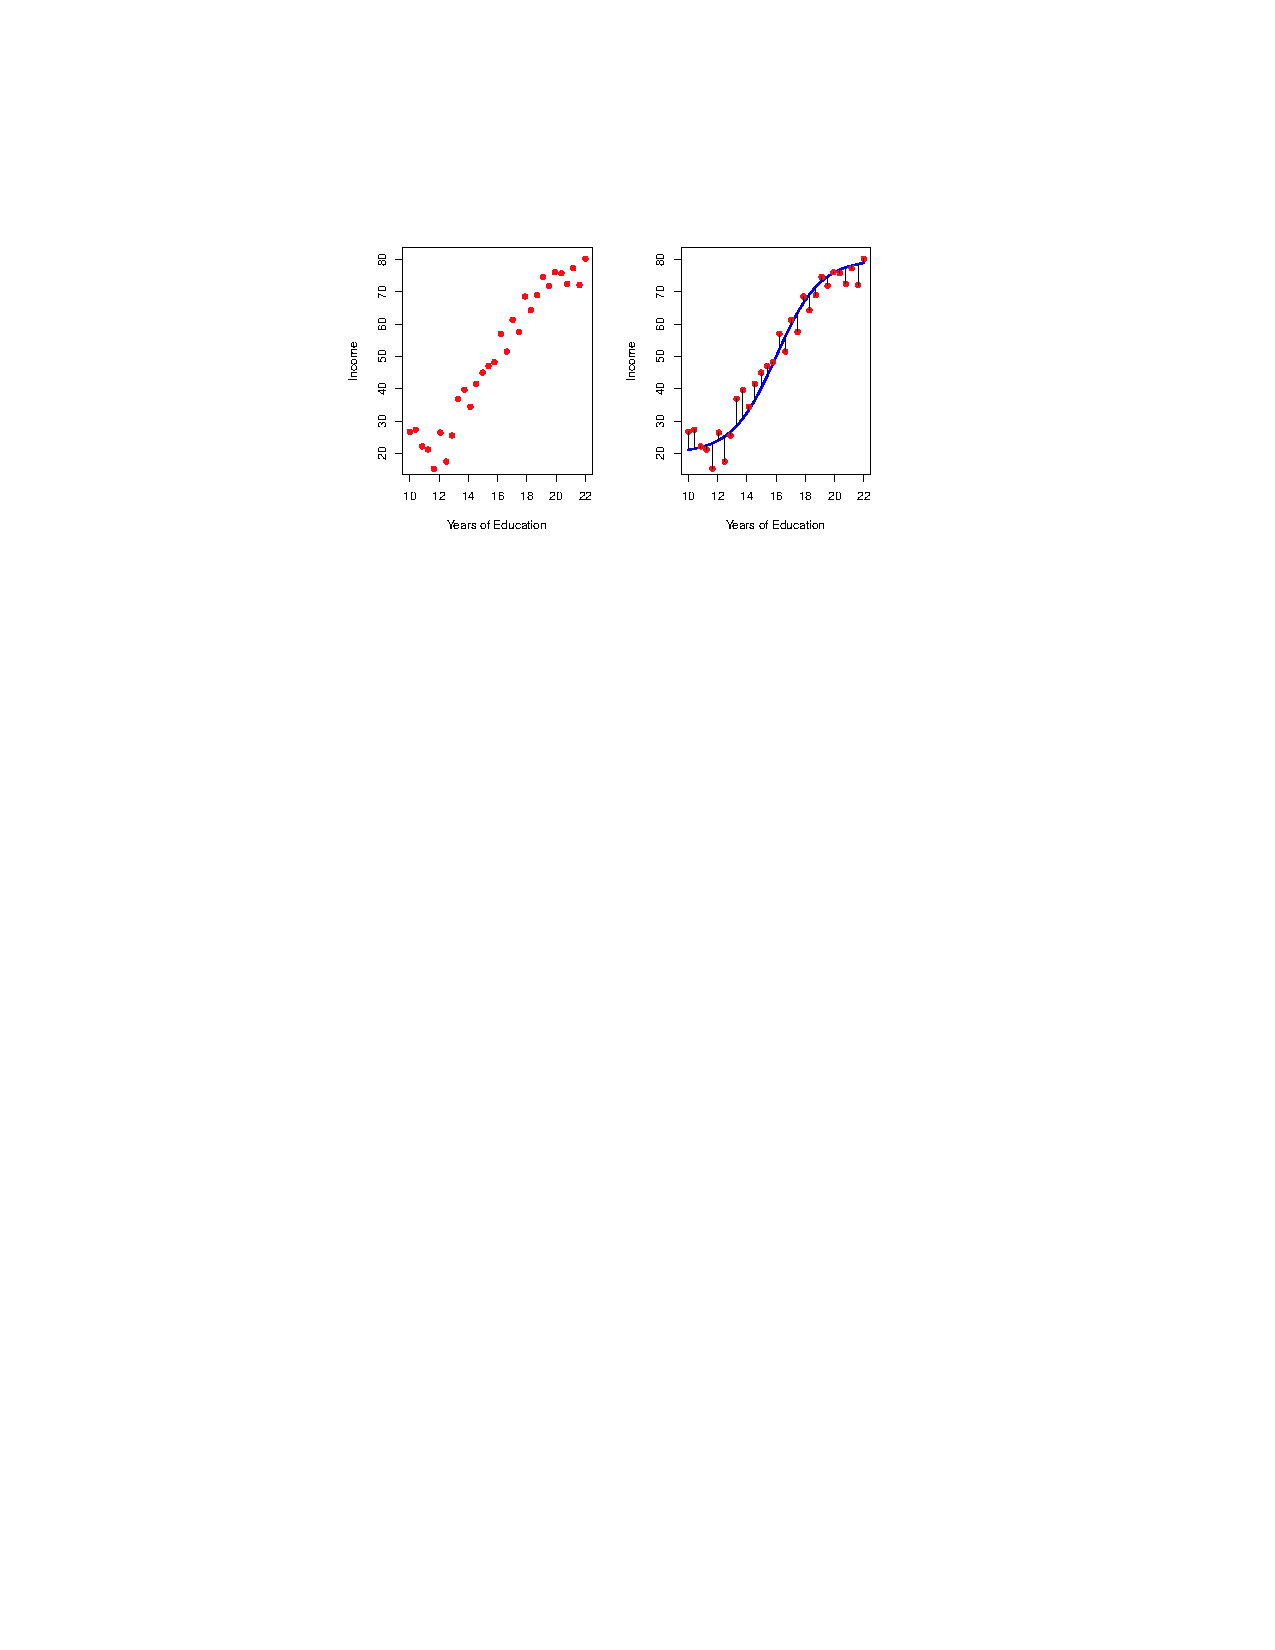
\includegraphics[width=\textwidth]{img/error-term-systematic-1.pdf}
                \captionof{figure}{The \texttt{Income} data set.\cite{james2013introduction}}
                \label{fig: error term systematic}
            \end{center}


            \noindent
            As you can see, the plot suggests that one might be able to predict \texttt{income} using \texttt{years of education}. Since \texttt{Income} is a simulated data set, the function $f$ is known and is shown by the blue curve in the right-hand panel. The \textbf{vertical lines} represent the \textbf{error terms} $\varepsilon$. We note that some of the 30 observations lie above the blue curve and some lie below it; overall, the \textbf{errors have approximately mean zero}.
        \end{examplebox}
    \end{figure}

    \noindent
    In essence, \textbf{statistical learning refers to a set of approaches for estimating $f$}. In this chapter we outline some of the key theoretical concepts that arise in estimating $f$.

    \newpage

    \subsection{Why Estimate \emph{f} (systematic information provided by a predictor about a quantitative response)?}

    There are two main reasons that we may wish to estimate $f$\index{systematic information}: \definition{prediction} and \definition{inference}.

    \longline

    \subsubsection{Prediction}\label{subsubsection: prediction}

    In many situations, a set of inputs $X$ are readily available, but the output $Y$ cannot be easily obtained. In this setting, since the error term $\varepsilon$ averages to zero, we can predict $Y$ using:
    \begin{equation}
        \hat{Y} = \hat{f}\left(X\right)
    \end{equation}
    \begin{itemize}
        \item $\hat{f}$ represents our \textbf{estimate for} $\bm{f}$
        \item $\hat{Y}$ represents \definition{prediction} for $Y$
    \end{itemize}
    The function $\hat{f}$ is often treated as a \textbf{black box}, in the sense that one is not typically concerned with the exact form of $\hat{f}$, provided that \textbf{it yields accurate predictions for} $Y$.

    \begin{examplebox}
        As an \example{example}, suppose that:
        \begin{itemize}
            \item $X_{1}, \dots, X_{p}$ are \textbf{characteristics of a patient's blood sample} that can be easily measured in a lab.
            \item $Y$ is a variable encoding the \textbf{patient's risk for a severe adverse reaction to a particular drug}.
        \end{itemize}
        It is natural to seek to predict $Y$ using $X$, since we can then avoid giving the drug in question to patients who are at high risk of an adverse reaction. That is, patients for whom the estimate of $Y$ is high.
    \end{examplebox}

    \noindent
    The accuracy of $\hat{Y}$ as a prediction for $Y$ depends on two quantities: \definition{reducible error} and \definition{irreducible error}.
    \begin{itemize}
        \item In general, $\hat{f}$ will not be a perfect estimate for $f$, and this \textbf{inaccuracy} will introduce some error. This is a \definition{reducible error} because we can potentially \textbf{improve the accuracy of $\bm{\hat{f}}$ by using the most appropriate statistical learning technique to estimate $\bm{f}$}.
        
        \item Even if it were possible to form a perfect estimate for $f$, so that our estimated response took the form $\hat{Y} = f\left(X\right)$, our prediction would still have some error in it! This is because $Y$ is also a function of $\varepsilon$ (error term), which, by definition, cannot be predicted using $X$. Therefore, variability associated with $\varepsilon$ also affects the accuracy of our predictions. This is the \definition{irreducible error}, because \textbf{no matter how well we estimate $\bm{f}$, we cannot reduce the error introduced by $\bm{\varepsilon}$}.
    \end{itemize}
    The real question is: \emph{why is the irreducible error larger than zero?} Well, the quantity $\varepsilon$ may contain unmeasured variables that are useful in predicting $Y$: since we don't measure them, $f$ cannot use them for its prediction. The quantity $\varepsilon$ may also contain unmeasurable variation.

    \begin{examplebox}
        For \example{example}, the risk of an adverse reaction might vary for a given patient on a given day, depending on manufacturing variation in the drug itself or the patient's general feeling of well-being on that day.
    \end{examplebox}

    \noindent
    Consider a given estimate $\hat{f}$ and a set of predictors $X$, which yields the prediction $\hat{Y} = \hat{f}\left(X\right)$. Assume for a moment that both $\hat{f}$ and $X$ are fixed, so that the only variability comes from $\varepsilon$ (error term). Then, it's easy to show that:
    \begin{equation}\label{eq: reducible and irreducible error}
        \begin{array}{rcl}
            E\left(Y - \hat{Y}\right)^{2} &=& E\left[f\left(X\right) + \varepsilon - \hat{f}\left(X\right)\right]^{2} \\ [1em]
                                          &=& \underbrace{\left[f\left(X\right) - \hat{f}\left(X\right)\right]^{2}}_{\text{Reducible}} + \underbrace{\Var\left(\varepsilon\right)}_{\text{Irreducible}}
        \end{array}
    \end{equation}
    \begin{itemize}
        \item $\left[f\left(X\right) - \hat{f}\left(X\right)\right]^{2}$ represents the \textbf{squared difference between the predicted and actual value of} $\bm{Y}$
        
        \item $E\left(Y-\hat{Y}\right)^{2}$ represents the \textbf{average}, or \definition{exprected value}
        
        \item $\Var\left(\varepsilon\right)$ represents the \definition{variance} \textbf{associated with the error term} $\bm{\varepsilon}$
    \end{itemize}
    The focus of this course is on \emph{techniques} for estimating $f$ with the aim of \textbf{minimizing the reducible error}. It is important to keep in mind that the irreducible error will always provide an upper bound on the accuracy of our prediction for $Y$. Unfortunately, this bound is almost always unknown in practice.

    \begin{examplebox}
        Consider a company that is interested in conducting a direct-marketing campaign.

        The \emph{goal} is to identify individuals who are likely to respond positively to a mailing, based on observations of demographic variables measured on each individual.

        In this case:
        \begin{itemize}
            \item The demographic variables serve as \emph{predictors};
            \item Response to the marketing campaign (either positive or negative) serves as the \emph{outcome}.
        \end{itemize}
        The company is \underline{not} interested in obtaining a deep understanding of the relationships between each individual predictor and the response; instead, the company simply \textbf{wants to accurately predict the response using the predictors}.

        This is an example of \textbf{modeling for prediction}.
    \end{examplebox}

    \subsubsection{Inference}\index{inference}\label{subsubsection: inference}

    We are often interested in understanding the association between $Y$ (quantitative response) and $X_{1}, \dots, X_{p}$ ($p$-predictors). In this situation we wish to estimate $f$ (systematic information), but our goal is not necessarily to make predictions for $Y$. Now it's obviously that $\hat{f}$ cannot be treated as a black box, because we need to know its exact form. In this setting, one may be interested in \textbf{answering the following questions}:
    \begin{itemize}
        \item \example{\emph{Which predictors are associated with the response?}} It is often the case that only a small fraction of the available predictors are substantially associated with $Y$. So, \textbf{identifying} the few \textbf{important predictors among a large set of possible variables can be extremely useful}.

        \item \example{\emph{What is the relationship between the response and each predictor?}} Larger values of the predictor are associated with larger values of $Y$. Other predictors may have the opposite relationship. The relationship between the response and the given predictor may \textbf{depend} on:
        \begin{itemize}
            \item The \textbf{complexity} of $f$;
            \item The \textbf{values of the other predictors}.
        \end{itemize}

        \item \example{\emph{Can the relationship between $Y$ and each predictor be adequately summarized using a linear equation, or is the relationship more complicated?}} Historically, \textbf{most methods} for estimating $f$ \textbf{have} taken \textbf{linear form}. But often the true relationship is more complicated, in which case a \textbf{linear model may not provide an accurate representation} of the relationship between the input and the output variables.
    \end{itemize}

    \begin{examplebox}
        Modeling the brand of a product that a customer might purchased based on variables such as:
            \begin{itemize}
                \item Price
                \item Store
                \item Location
                \item Discount levels
                \item Competition price
            \end{itemize}
        And so forth. In this situation one might really be most interested in the \textbf{association between each variable and the probability of purchase}. For instance, \emph{to what extent is the product's price associated with sales?}

        This is an example of \textbf{modeling for inference}.
    \end{examplebox}

    \newpage

    \begin{figure}[!htp]
        \begin{examplebox}
            Consider the following figure:
            \begin{center}
                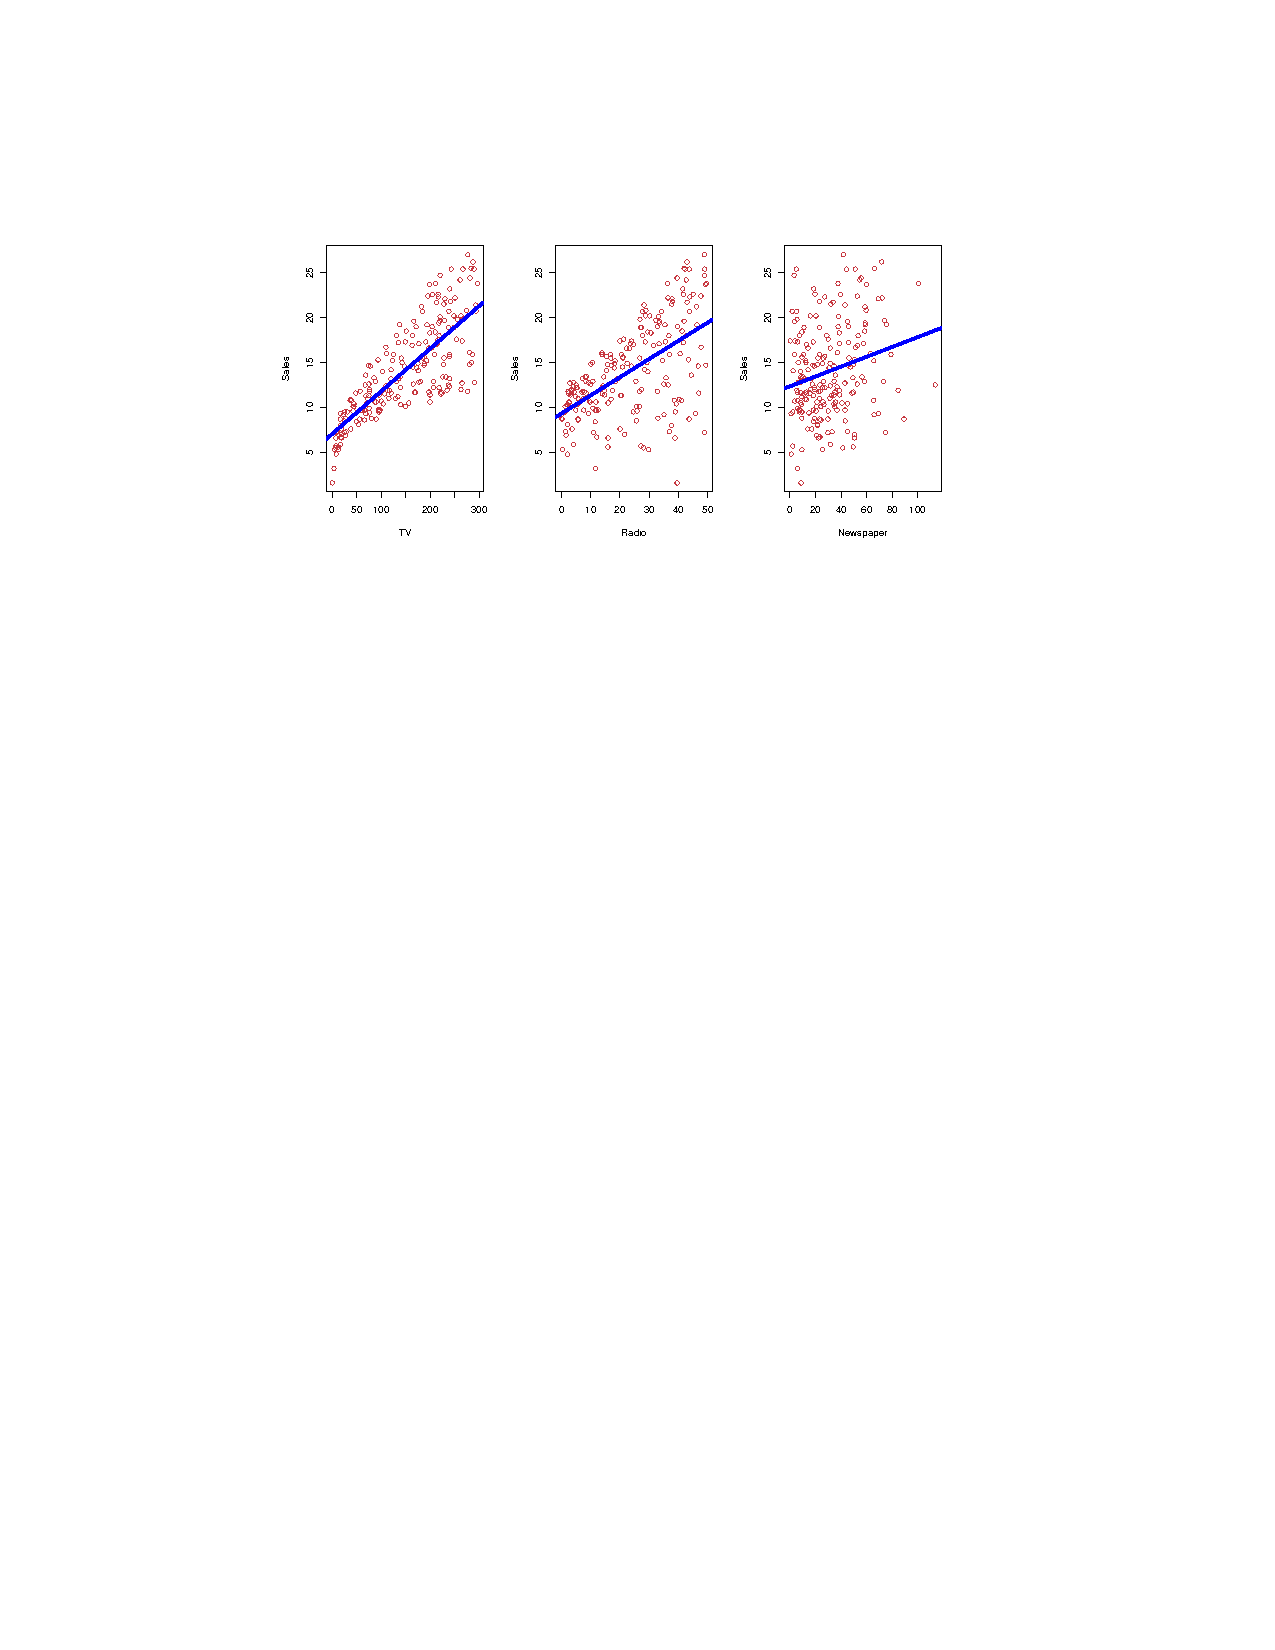
\includegraphics[width=\textwidth]{img/statistical-learning-1.pdf}
                \captionof{figure}{The \texttt{Advertising} data set. The plot displays \texttt{sales}, in thousands of units, as a function of \texttt{TV}, \texttt{radio}, and \texttt{newspaper} budgets, in thousands of dollars, for 200 different markets. In each plot we show the simple least squares fit of \texttt{sales} to that variable. In other words, each blue line represents a simple model that can be used to predict \texttt{sales} using \texttt{TV}, \texttt{radio}, and \texttt{newspaper}, respectively.}
            \end{center}
            One may be interested in answering questions such as:
            \begin{itemize}
                \item \emph{Which media are associated with sales?}
                \item \emph{Which media generate the biggest boost in sales?}
                \item \emph{How large of an increase in sales is associated with a given increase in TV advertising?}
            \end{itemize}
            This situation falls into the \textbf{inference model}.
        \end{examplebox}
    \end{figure}

    \newpage

    \subsubsection{Difference between prediction and inference}

    \begin{examplebox}
        In a real estate setting, one may seek to relate values of homes to inputs such as:
        \begin{itemize}
            \item Crime rate
            \item Zoning
            \item Distance from a river
            \item Air quality
            \item Schools
            \item Income level of community
            \item Size of houses
        \end{itemize}
        And so forth. In this case one might be interested in the association between each individual input variable and housing price. For instance, \emph{how much extra will a house be worth if it has a view of the river?} This is an \textbf{inference problem}.

        \vspace{.5em}
        But \underline{attention}! Alternatively, one may simply be interested in predicting the value of a home given its characteristics: \emph{is this house under or over valued?} And this is a \textbf{prediction problem}.
    \end{examplebox}

    So, as you can see from the example, the difference between a prediction problem and an inference problem is so small. A problem can change its nature because the ultimate goal is also changing.

    \newpage

    \subsection{How do we estimate \emph{f}?}

    We will always assume that we have observed a set of $n$ different data points. For example, in figure~\ref{fig: error term systematic} at page~\pageref{fig: error term systematic} we observed $n=30$ data points. These observations are called \definition{training data} because we will \textbf{use these observations to train, or teach, our method how to estimate} $\bm{f}$.
    
    \highspace
    Let:
    \begin{itemize}
        \item $x_{ij}$ represent the value of the $j$th predictor, or input, for observation $i$, where $i=1,2,\dots,n$ and $j=1,2,\dots,p$
        
        \item $y_{i}$ represent the response variable for the $i$th observation.
    \end{itemize}
    Then, our training data consist of:
    \begin{equation*}
        \left\{\left(x_{1}, y_{1}\right), \left(x_{2}, y_{2}\right), \dots, \left(x_{n}, y_{n}\right)\right\}
    \end{equation*}
    Where $x_{i} = \left(x_{i1}, x_{i2}, \dots, x_{ip}\right)^{T}$.
    
    \highspace
    Our \underline{goal} is to \textbf{apply a statistical learning method to the training data in order to estimate the unknown function} $\bm{f}$. In other words, we want to find a function $\hat{f}$ such that $Y \approx \hat{f}\left(X\right)$ for any observations $\left(X, Y\right)$. Most statistical learning methods for this task can be characterized as either \definition{parametric} or \definition{non-parametric}.
    
    \newpage

    \subsubsection{Parametric Methods}

    The \definition{parametric methods} involve a two-step model-based approach:
    \begin{enumerate}
        \item Select a model.
        \begin{enumerate}
            \item \textbf{Make an assumption about the functional form}, or shape, of $f$. For \example{example}, one very simple assumption is that $f$ is linear in $X$:
            \begin{equation}
                f\left(X\right) = \beta_{0} + \beta_{1}X_{1} + \beta_{2}X_{2} + \cdots + \beta_{p}X_{p}
            \end{equation}
            This is a \definition{linear model} (that will be discussed in the future). Once we have assumed that $f$ is linear, \textbf{the problem of estimating $\bm{f}$ is greatly simplified}. Instead of having to estimate an entirely arbitrary $p$-dimensional function $f\left(X\right)$, one only needs to \textbf{estimate the $\bm{p+1}$ coefficients} $\beta_{0}, \beta_{1}, \dots, \beta_{p}$.
        \end{enumerate}

        \item Use training data to fit/train the model.
        \begin{enumerate}
            \item[(b)] After a model has been selected, we need a \textbf{procedure that uses the training data to} \definition{fit the model} or \definition{train the model}. In the case of the linear method, we need to estimate the parameters $\beta_{0}, \beta_{1}, \dots, \beta_{p}$. So, we want to find values of these parameters such that:
            \begin{equation*}
                Y \approx \beta_{0} + \beta_{1}X_{1} + \beta_{2}X_{2} + \cdots + \beta_{p}X_{p}
            \end{equation*}
            The most \textbf{common approach to fitting} the (linear) model is referred to as (\textbf{ordinary}) \definition{least squares} (that will be discussed in the future). However, the least squares is one of many possible ways to fit the linear model.
        \end{enumerate}
    \end{enumerate}
    The parametric model-based reduces the problem of estimating $f$ down to one of \textbf{estimating a set of parameters}. In fact, assuming a parametric form for $f$ simplifies the problem of estimating $f$ because it is generally much easier to estimate a set of parameters in the linear model, than it is to fit an entirely arbitrary function $f$.

    \begin{flushleft}
        \textcolor{Red2}{\faIcon{exclamation-triangle} \textbf{Potential disadvantage}}
    \end{flushleft}
    The \textbf{model} we choose will \textbf{usually not match the true unknown form of} $\bm{f}$. If the chosen model is \textbf{too far} from the true $f$, then our \textbf{estimate will be poor}.

    \begin{flushleft}
        \textcolor{Green3}{\faIcon{check} \textbf{Possible (partial) solution}}
    \end{flushleft}
    We can try to address this problem by \textbf{choosing} \definition{flexible models} that can \textbf{fit many different possible functional forms for} $\bm{f}$. But fitting a more flexible model \textbf{requires estimating a greater number of parameters}. 
    
    These more complex models (\textbf{flexible models}) can lead to a phenomenon known as \definition{overfitting} the data, which essentially means \textbf{they follow the errors}, or \definition{noise}, \textbf{too closely} (these issues are discussed throughout this course).

    \newpage

    \subsubsection{Non-Parametric Methods}

    The \definition{non-parametric} methods do not make explicit assumptions about the functional form of $f$. Instead they seek an \textbf{estimate of} $\bm{f}$ \textbf{that gets as close to the data points as possible without being too rough or wiggly}.

    \begin{flushleft}
        \textcolor{Green3}{\faIcon{check} \textbf{Major advantage over parametric approaches}}
    \end{flushleft}
    By avoiding the assumption of a particular functional form for $f$, non-parametric approaches have the \textbf{potential to accurately fit a wider range of possible shapes} for $f$. Any parametric approach brings with it the possibility that the functional form used to estimate $f$ is very different from the true $f$, in which case the resulting model will not fit the data well.

    \begin{flushleft}
        \textcolor{Red2}{\faIcon{exclamation-triangle} \textbf{Disadvantage}}
    \end{flushleft}
    Since non-parametric approaches do not reduce the problem of estimating $f$ to a small number of parameters, \textbf{a very large number of observations} (far more than is typically needed for a parametric approach) \textbf{is required in order to obtain an accurate estimate} for $f$.

    \newpage

    \subsection{Supervised and Unsupervised Learning}

    Most statistical learning problems fall into one of two categories: \definition{supervised learning} or \definition{unsupervised learning}.

    \longline

    \begin{flushleft}
        \large
        \textbf{Supervised learning}
    \end{flushleft}
    The examples that we have discussed in this chapter all fall into the \definition{supervised learning} domain. For each observation of the predictor measurement(s) $x_{i}, i=1,\dots,n$ there is an associated response measurement $y_{i}$.

    \highspace
    We wish to \textbf{fit a model that relates the response to the predictors}, with the \underline{aim} of:
    \begin{itemize}
        \item \textbf{Accurately predicting the response for future observations} (prediction, section~\ref{subsubsection: prediction})
        \item \textbf{Better understanding the relationship between the response and the predictors} (inference, section~\ref{subsubsection: inference})
    \end{itemize}

    \longline
    
    \begin{flushleft}
        \large
        \textbf{Unsupervised learning}
    \end{flushleft}
    The \definition{unsupervised learning} describes the somewhat more challenging situation in which \textbf{for every observation} $i=1,\dots,n$, \textbf{we observe a vector of measurements} $x_{i}$ \textbf{but no associated response} $y_{i}$. 
    
    \highspace
    In this setting, we are in some sense \emph{working blind}; the situation is referred to as \textbf{unsupervised} because \textbf{we lack a response variable that can supervise our analysis}. We can \textbf{seek to understand the relationships between the variables or between the observations}.

    \newpage

    \subsection{Assessing Model Accuracy}

    The aim of this section is to decide which method will give the best results for a given set of data.

    \subsubsection{Measuring the Quality of Fit (MSE)}

    In order to evaluate the performance of a statistical learning method on a given data set, we need some way to measure how well its predictions actually match the observed data. We need to \textbf{quantify the extent to which the predicted response value for a given observation is close to the true response value for that observation}. The most commonly-used measure is the \definition{mean squared error (MSE)}:
    \begin{equation}\label{eq: mean squared error}
        \mathrm{MSE} = \dfrac{1}{n} \displaystyle\sum_{i=1}^{n} \left(y_{i} - \hat{f}\left(x_{i}\right)\right)^{2}
    \end{equation}
    \begin{itemize}
        \item $\hat{f}\left(x_{i}\right)$ is the prediction that $\hat{f}$ gives for the $i$th observation
        \item $y_{i}$ the $i$th true response
    \end{itemize}
    Obviously,the MSE will be:
    \begin{itemize}
        \item \textbf{Small} if the predicted responses are very close to the true responses;
        \item \textbf{Large} if for some of the observations, the predicted and true responses differ substantially.
    \end{itemize}
    In general, we do not really care how well the method works on the training data. Rather, \textbf{we are interested in the accuracy of the predictions that we obtain when we apply our method to previously unseen test data}.

    \begin{examplebox}
        Suppose that we are interested in developing an algorithm to predict a stock's price based on previous stock returns.

        \highspace
        We can train the method using stock returns from the past 6 months. But we \underline{don't} really care how well our method predicts last week's stock price.

        We instead \textbf{care about how well it predict tomorrow's price or next month's price}.
    \end{examplebox}

    \newpage

    \begin{examplebox}
        Suppose that we have clinical measurements (e.g. weight, blood pressure, height, age, family history of disease) for a number of patients, as well as information about whether each patient has diabetes.

        \highspace
        We can use these patients to train a statistical learning method to predict risk of diabetes based on clinical measurements.

        \highspace
        In practice, \textbf{we want this method to accurately predict diabetes risk for \emph{future patients} based on their clinical measurements}. Again, we are \underline{not} very interested in whether or not the method accurately predicts diabetes risk for patients used to train the mode, since \underline{we already know which of those patients have diabetes}!
    \end{examplebox}

    \noindent
    In mathematical terms, suppose that we fit our statistical learning method on our training observations:
    \begin{equation*}
        \left\{\left(x_{1}, y_{1}\right), \left(x_{2}, y_{2}\right), \dots, \left(x_{n}, y_{n}\right)\right\}
    \end{equation*}
    And we obtain the estimate $\hat{f}$. We can then compute:
    \begin{equation*}
        \hat{f}\left(x_{1}\right), \hat{f}\left(x_{2}\right), \dots, \hat{f}\left(x_{n}\right)
    \end{equation*}
    If these are approximately equal to:
    \begin{equation*}
        y_{1}, y_{2}, \dots, y_{n}
    \end{equation*}
    Then \textbf{the training MSE is small}.

    \highspace
    However, we are really \underline{not interested} in whether $\hat{f}\left(x_{i}\right) \approx y_{i}$; instead, we want to know whether $\hat{f}\left(x_{0}\right)$ is approximately equal to $y_{0}$, where $\left(x_{0}, y_{0}\right)$ is a \textbf{previously unseen test observation not used to train the statistical learning method}.

    We \textbf{want to choose the method that gives the lowest} \definition{test mean squared error (MSE)}, as opposed to the lowest training MSE. In other words, if we had a large number of test observations, we could compute:
    \begin{equation}
        \mathrm{Ave}\left(y_{0} - \hat{f}\left(x_{0}\right)\right)^{2}
    \end{equation}
    The \textbf{average squared prediction error for these test observations} $\left(x_{0}, y_{0}\right)$.

    \begin{flushleft}
        \textcolor{Red2}{\faIcon{exclamation-triangle} \textbf{Problem to find the lowest training MSE}}
    \end{flushleft}
    There is \underline{no guarantee} that the method with the lowest training MSE will also have the lowest test MSE. 
    
    The problem is that \textbf{many statistical methods specifically estimate coefficients so as to minimize the training set MSE}. For these methods, the \textbf{training set MSE can be quite small}, \textbf{but the test MSE is often much larger}.
    
    \newpage

    \begin{figure}[!htp]
        \begin{examplebox}
            \begin{center}
                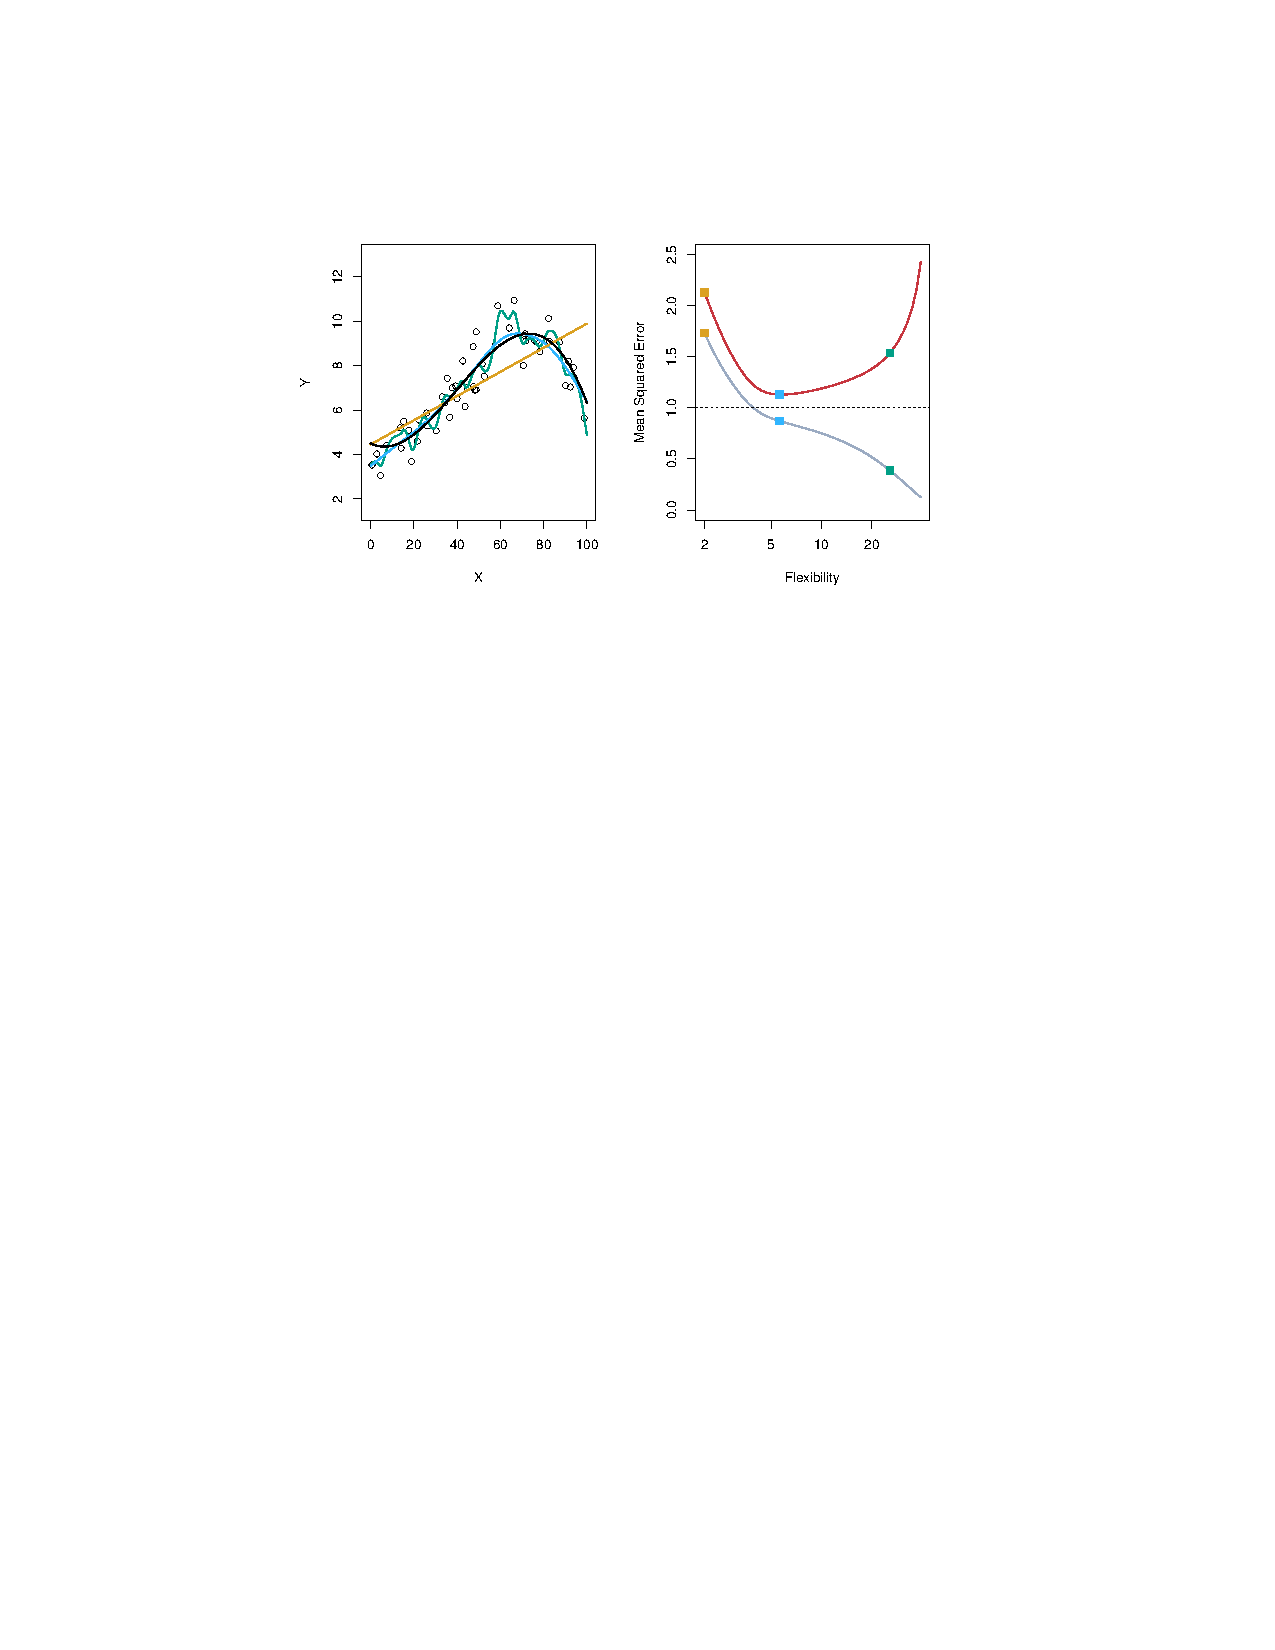
\includegraphics[width=\textwidth]{img/measuring-the-quality-of-fit-1.pdf}
                \captionof{figure}{On the left: \emph{data simulated from $f$, shown in black. Three estimates of $f$ are shown: the linear regression (orange curve), and two smoothing spline fits (blue and green curves)}. Right: \emph{Training MSE (grey curve), test MSE (red curve), and minimum possible test MSE over all methods (dashed line). Squares represent the training and test MSEs for the three fits shown in the left-hand panel}.\cite{james2013introduction}}
                \label{fig: measuring the quality of fit}
            \end{center}
            In the left-hand panel we have generated observations from the (error term\index{error term}) equation~\ref{eq: error term systematic} with the true $f$ given by the black curve. 
            
            The orange, blue and green curves illustrate three possible estimates for $f$ obtained using methods with increasing levels of flexibility.

            \highspace
            It is clear that as the \textbf{level of flexibility increases}, the \textbf{curves fit the observed data more closely}. 
            
            The \emph{green curve} is the most flexible and matches the data very well; however, we observe that it fits the true $f$ (shown in black) poorly because it is too wiggly. 
            
            By \textbf{adjusting the level of flexibility} of the smoothing spline fit, we can \textbf{produce many different fits to this data}.
        \end{examplebox}
    \end{figure}

    \setcounter{example}{9}
    \newpage

    \begin{examplebox}
        \begin{center}
            Referring to Figure~\ref{fig: measuring the quality of fit}
        \end{center}

        We now move on to the right-hand panel. The grey curve displays the average training MSE as a function of flexibility, or more formally the \definition{degrees of freedom}\footnote{The degrees of freedom is a \textbf{quantity that summarizes the flexibility of a curve}.}, for a number of smoothing splines.

        The orange, blue and green squares indicate the MSEs associated with the corresponding curve in the left-hand panel.

        A more restricted and hence smoother curve has fewer degrees of freedom than a wiggly curve. The \emph{linear regression} is at the most restrictive end, with two degrees of freedom.

        \highspace
        The \textbf{training MSE declines monotonically as flexibility increases}. In this example, the true $f$ is non-linear, and so the orange linear fit is not flexible enough to estimate $f$ well. 
        
        The \emph{green curve} has the lowest training MSE of all three methods, since it corresponds to the most flexible of the three curves fit in the left-hand panel.

        \highspace
        The test MSE is displayed using the red curve. As with the training MSE, the test MSE initially declines as the level of flexibility increases.

        At some point, the test MSE levels off and then starts to increase again. Consequently, the orange and green curves both have high test MSE. The blue curve minimizes the test MSE, which should not be surprising given that visually it appears to estimate $f$ the best in the left-hand panel.

        The horizontal dashed line indicates $\Var\left(\varepsilon\right)$, the \textbf{irreducible error} (eq.~\ref{eq: reducible and irreducible error}), which \textbf{corresponds to the lost achievable test MSE among all possible methods}. Hence, the smoothing spline represented by \textbf{the blue curve is close to optimal}.
    \end{examplebox}

    In the right-hand panel of figure~\ref{fig: measuring the quality of fit}, as the flexibility of the Statistical learning method increases, we observe a \textbf{monotone decrease in the training MSE and a U-shape} in the test MSE. This is a \textbf{fundamental property} of statistical learning that holds regardless of the particular data set at hand and regardless of the Statistical method being used.
    
    As model flexibility increases, the training MSE will decrease, but the test MSE may not. \textbf{When a given method yields a small training MSE but a large test MSE}, we are said to be \definition{overfitting} the data.

    \begin{flushleft}
        \textcolor{Green3}{\faIcon{question-circle} \textbf{Why does this phenomenon happen?}}
    \end{flushleft}
    This happens because our \textbf{statistical learning procedure} is working too hard to find patterns in the training data, and \textbf{may be picking up some patterns that are just caused by random chance} rather than by true properties of the unknown function $f$.

    \noindent
    So when we \emph{overfit} the training data, the \textbf{test MSE} will be \textbf{very large because the supposed patterns that the method found in the training data simply don't exist in the test data}.

    \highspace
    We almost \underline{always} expect the \textbf{training MSE to be smaller than the test MSE} because most \textbf{statistical learning methods} either directly or indirectly seek to \textbf{minimize the training MSE}. \emph{Overfitting} refers specifically to the test case in which a \textbf{less flexible model would have yielded a smaller test MSE}.

    \begin{figure}[!htp]
        \begin{examplebox}
            \begin{center}
                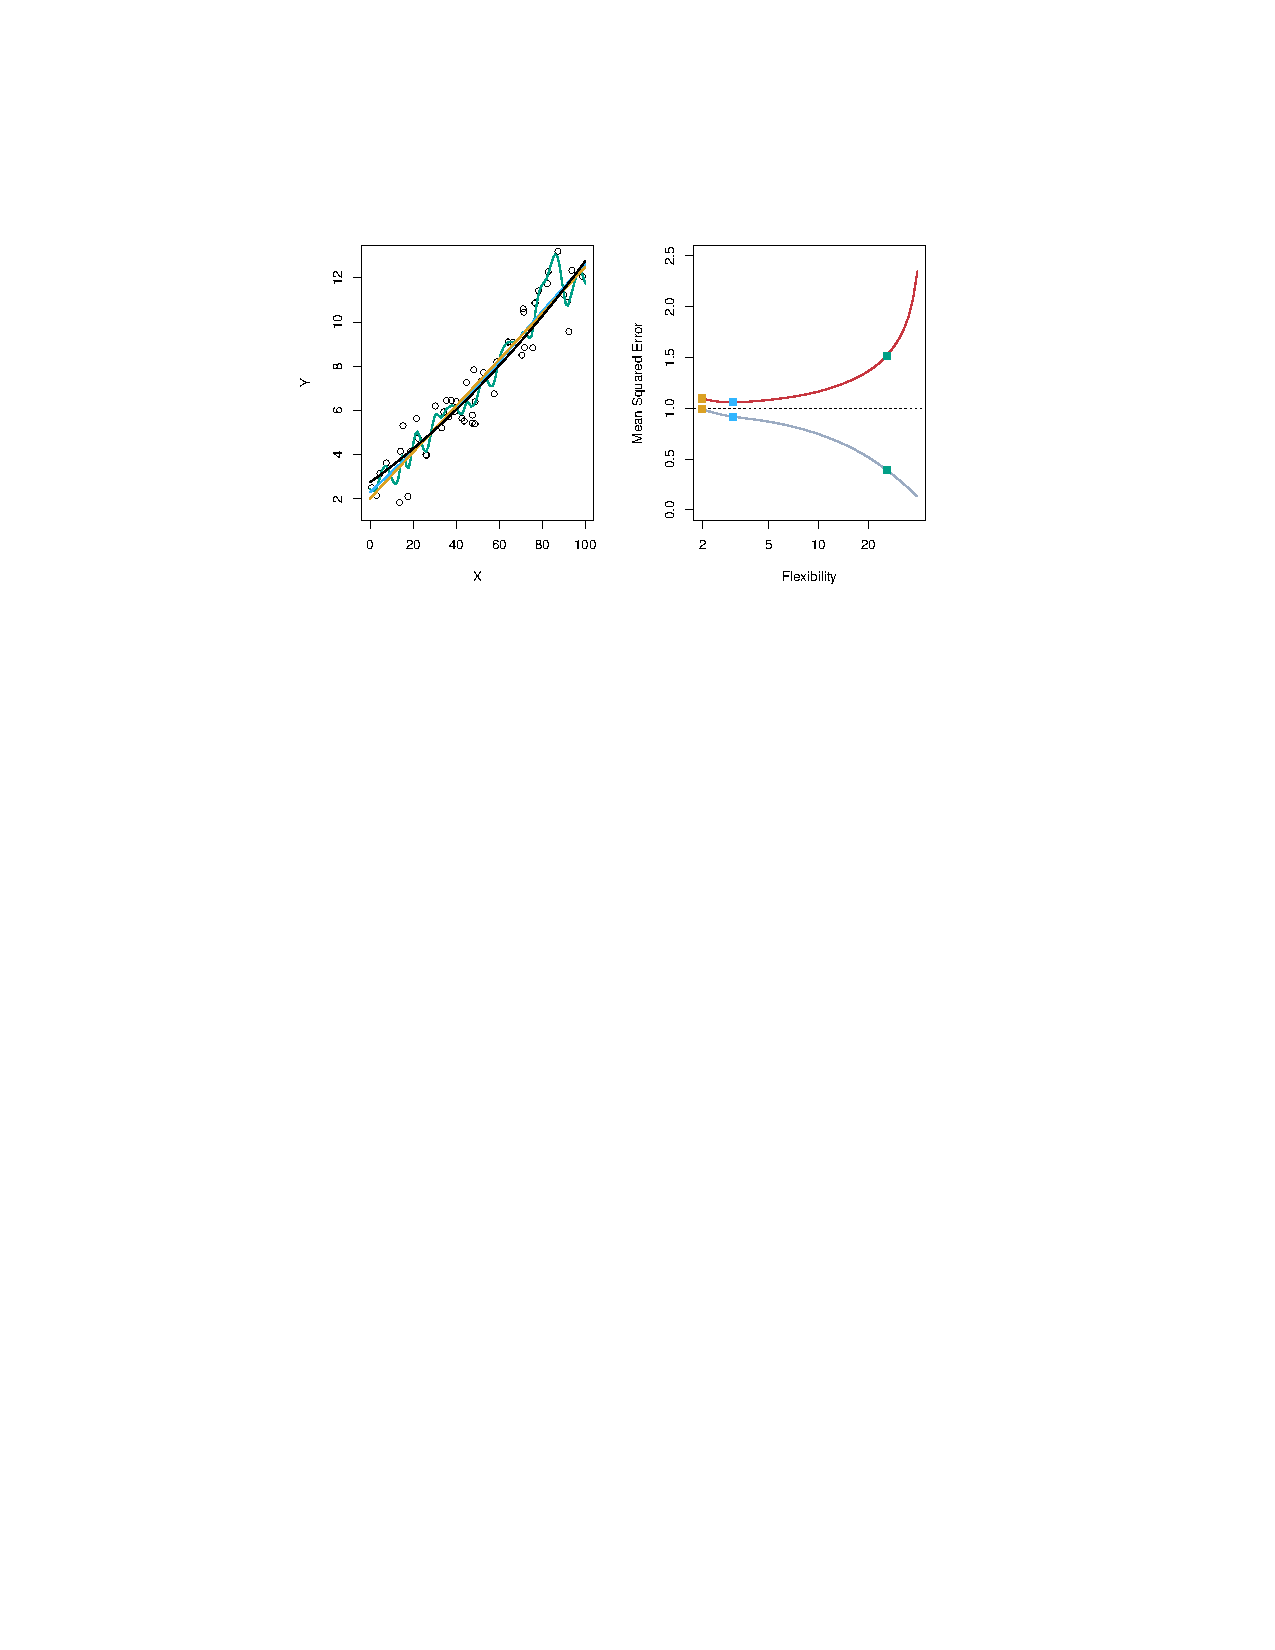
\includegraphics[width=\textwidth]{img/measuring-the-quality-of-fit-2.pdf}
                \captionof{figure}{Details are as in Figure~\ref{fig: measuring the quality of fit}, using a different true $f$ that is much closer to linear. In this setting, linear regression provides a very good fit to the data.\cite{james2013introduction}}
                \label{fig: measuring the quality of fit - 2}
            \end{center}

            This figure provides another \example{example} in which the true $f$ is approximately linear. Again we observe that the training MSE decreases monotonically as the model flexibility increases, and that there is a \emph{U-shape} in the test MSE. 
            
            \highspace
            However, because the truth is close to linear, the \textbf{test MSE only decreases slightly before increasing again}, so that the \textbf{orange least squares fit is substantially better than the highly flexible green curve}.
        \end{examplebox}
    \end{figure}

    \newpage

    \begin{figure}[!htp]
        \begin{examplebox}
            \begin{center}
                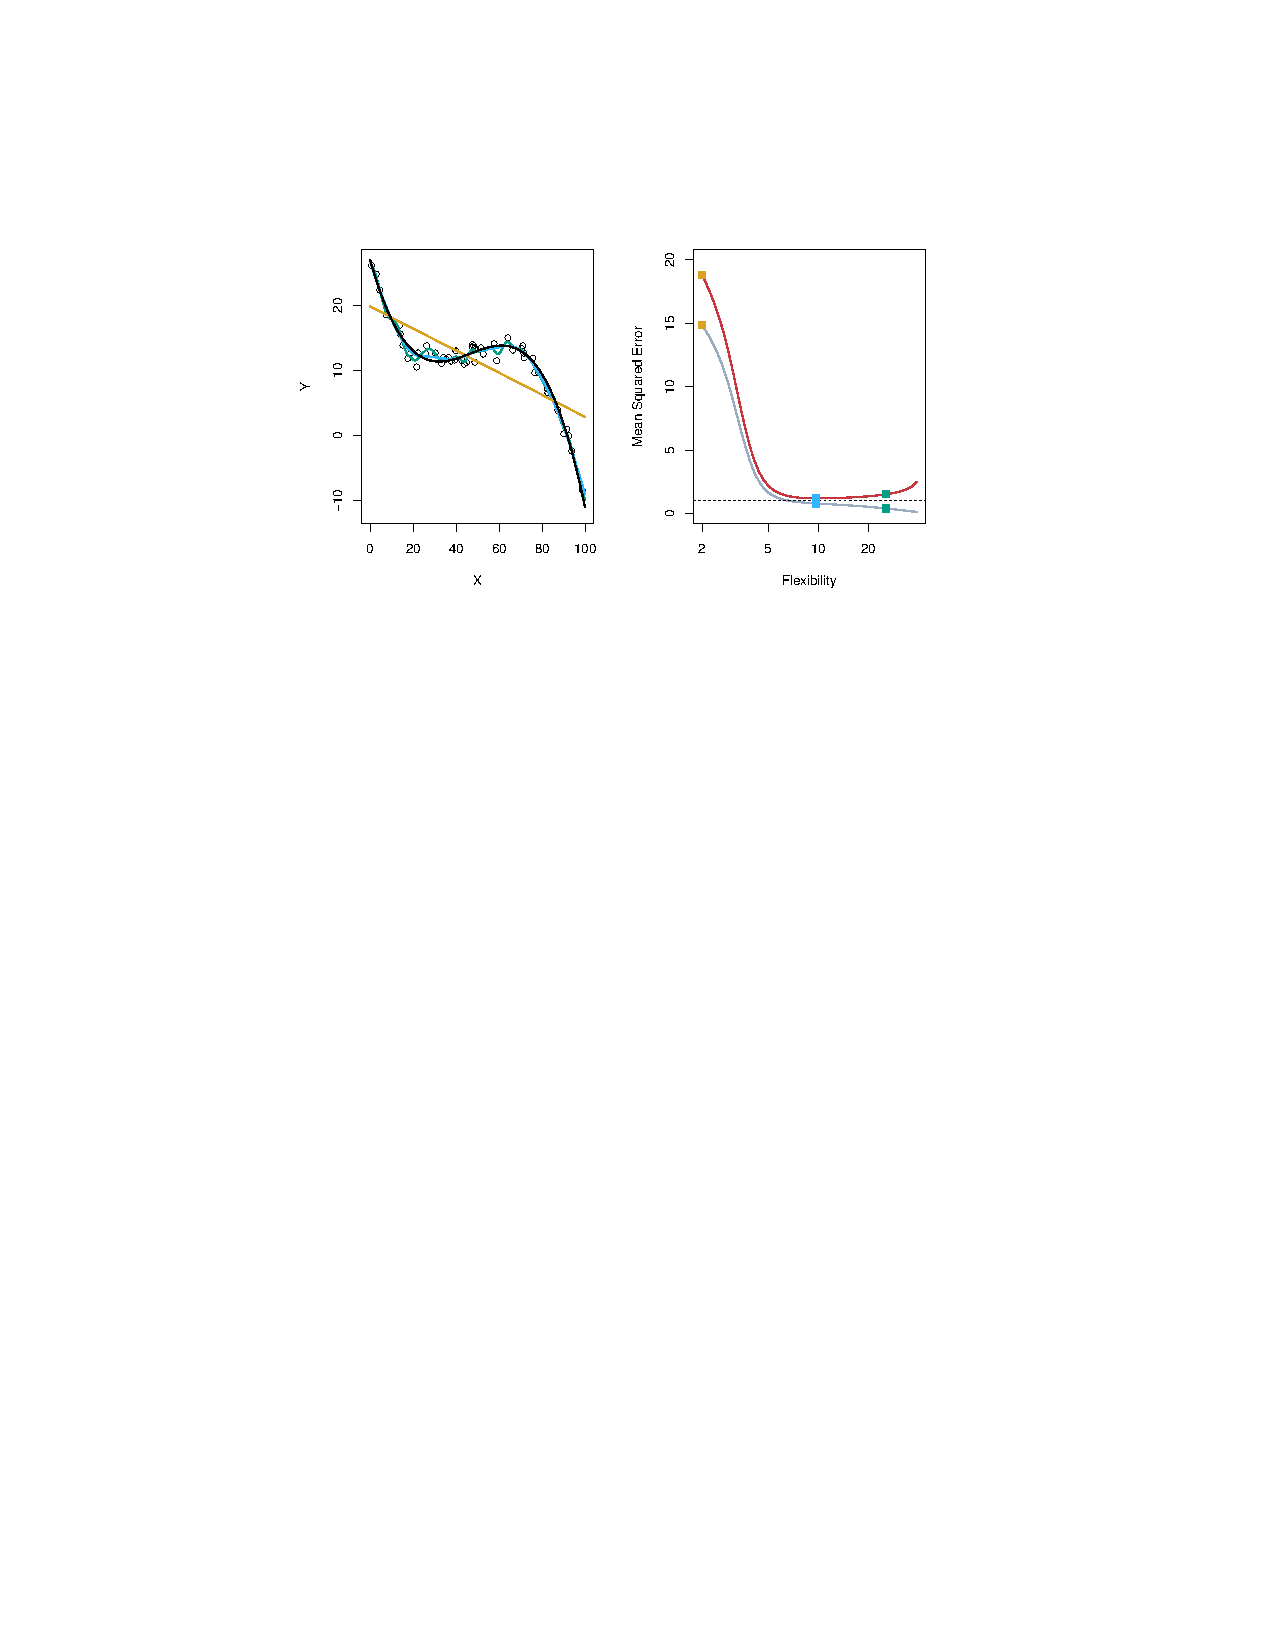
\includegraphics[width=\textwidth]{img/measuring-the-quality-of-fit-3.pdf}
                \captionof{figure}{Details are as in Figure~\ref{fig: measuring the quality of fit}, using a different true $f$ that is far from linear. In this setting, linear regression provides a very poor fit to the data.\cite{james2013introduction}}
                \label{fig: measuring the quality of fit - 3}
            \end{center}

            Finally, this figure displays an \example{example} in which $f$ is highly non-linear.

            \highspace
            The training and test MSE curves still exhibit the same general patterns, but now there is a rapid decrease in both curves before the test MSE start to increase slowly.
        \end{examplebox}
    \end{figure}
    
    \newpage

    \subsubsection{The Bias-Variance Trade-Off}

    The U-shape observed in the test MSE curves (Figures: \ref{fig: measuring the quality of fit}, \ref{fig: measuring the quality of fit - 2}, \ref{fig: measuring the quality of fit - 3}) turns out to be the result of two competing properties of statistical learning methods. 
    
    \highspace
    The expected test MSE, for a given value $x_{0}$, can always be decomposed into the sum of three fundamental quantities:
    \begin{itemize}
        \item The \definition{variance} of $\hat{f}\left(x_{0}\right)$
        
        \item The squared \definition{bias} of $\hat{f}\left(x_{0}\right)$
        
        \item The \textbf{variance of the error terms} $\bm{\varepsilon}$
    \end{itemize}
    \begin{equation}\label{eq: expected test MSE}
        E\left(y_{0} - \hat{f}\left(x_{0}\right)\right)^{2} = \Var\left(\hat{f}\left(x_{0}\right)\right) + \left[\Bias\left(\hat{f}\left(x_{0}\right)\right)\right]^{2} + \Var\left(\varepsilon\right)
    \end{equation}
    Where $E\left(y_{0} - \hat{f}\left(x_{0}\right)\right)^{2}$ defines the \definition{expected test MSE} at $x_{0}$ and refers to the \textbf{average test MSE} that we would obtain if we \textbf{repeatedly estimated} $\bm{f}$ \textbf{using a large number of training sets, and tested each at} $x_{0}$.

    \highspace
    The equation \ref{eq: expected test MSE} tell us that in order to minimize the expected test error, we need to \textbf{simultaneously select a statistical learning method that} achieves \textbf{\underline{low} variance and \underline{low} bias}. Note that variance is inherently a nonnegative quantity, and squared bias is also nonnegative. Hence, we see that the expected test MSE can never lie below $\Var\left(\varepsilon\right)$, the irreducible error (equation~\ref{eq: reducible and irreducible error}).

    \begin{flushleft}
        \textcolor{Red2}{\faIcon[regular]{star} \textbf{Meaning of the variance}}
    \end{flushleft}
    The \definition{variance} refers to the \textbf{amount by which} $\bm{\hat{f}}$ \textbf{would change if we estimated it using a different training data set}. So different training data sets will result in a different $\hat{f}$. But ideally the estimate for $f$ should not vary too much between training sets. However, \textbf{if a method has high variance then small changes in the training data can result in large changes in} $\bm{\hat{f}}$. 
    
    \noindent
    In general, \textbf{more flexible statistical methods have higher variance}.

    \begin{examplebox}
        Consider the green and the orange curves in Figure~\ref{fig: measuring the quality of fit} at page~\pageref{fig: measuring the quality of fit}.
        
        \highspace
        The flexible green curve is following the observations very closely. It has high variance because changing any one of these data points may cause the estimate $\hat{f}$ to change considerably. 
        
        \highspace
        In contrast, the orange least squares line is relatively inflexible and has low variance, because moving any single observations will likely cause only a small shift in the position of the line.
    \end{examplebox}

    \newpage

    \begin{flushleft}
        \textcolor{Red2}{\faIcon[regular]{star} \textbf{Meaning of the bias}}
    \end{flushleft}
    The \definition{bias} refers to the \textbf{error that is introduced by approximating a real-life problem, which may be extremely complicated, by a much simpler model}.

    \begin{examplebox}
        For \example{example}, linear regression assumes that there is a linear relationship between $Y$ and $X_{1}, X_{2}, \dots, X_{p}$. It is unlikely that any real-life problem truly has such a simple linear relationship, and so performing linear regression will undoubtedly result in some bias in the estimate of $f$.

        \highspace
        In the Figure~\ref{fig: measuring the quality of fit - 3} on page \pageref{fig: measuring the quality of fit - 3}, the true $f$ is substantially non-linear, so no matter how many training observations we are given, it will not be possible to produce an accurate estimate using linear regression. In other words, linear regression results in high bias in this example.

        \highspace
        However, in Figure~\ref{fig: measuring the quality of fit - 2} on page \pageref{fig: measuring the quality of fit - 2} the true $f$ is very close to linear, and so given enough data, it should be possible for linear regression to produce an accurate estimate.
    \end{examplebox}

    \noindent
    Generally, as we use \textbf{more flexible methods}, the \definition{variance} \textbf{will increase} and the \definition{bias} \textbf{will decrease}.

    \highspace
    As we increase the flexibility of a class of methods, the bias tends to initially decrease faster than the variance increases. Consequently, the expected test MSE declines. However, at some point increasing flexibility has little impact on the bias but starts to significantly increase the variance. When this happens the test MSE increases. Note that we observed this pattern of decreasing test MSE followed by increasing test MSE in the right-hand panels of Figures \ref{fig: measuring the quality of fit}, \ref{fig: measuring the quality of fit - 2}, \ref{fig: measuring the quality of fit - 3}. In summary:
    \begin{enumerate}
        \item We increase the flexibility of a class of methods;
        \item The bias tends to initially decrease faster than the variance increases;
        \item The expected test MSE declines;
        \item At some point increasing flexibility has little impact on the bias but starts to significantly increase the variance;
        \item The test MSE increases.
    \end{enumerate}

    \newpage

    \begin{figure}[!htp]
        \begin{examplebox}
            \begin{center}
                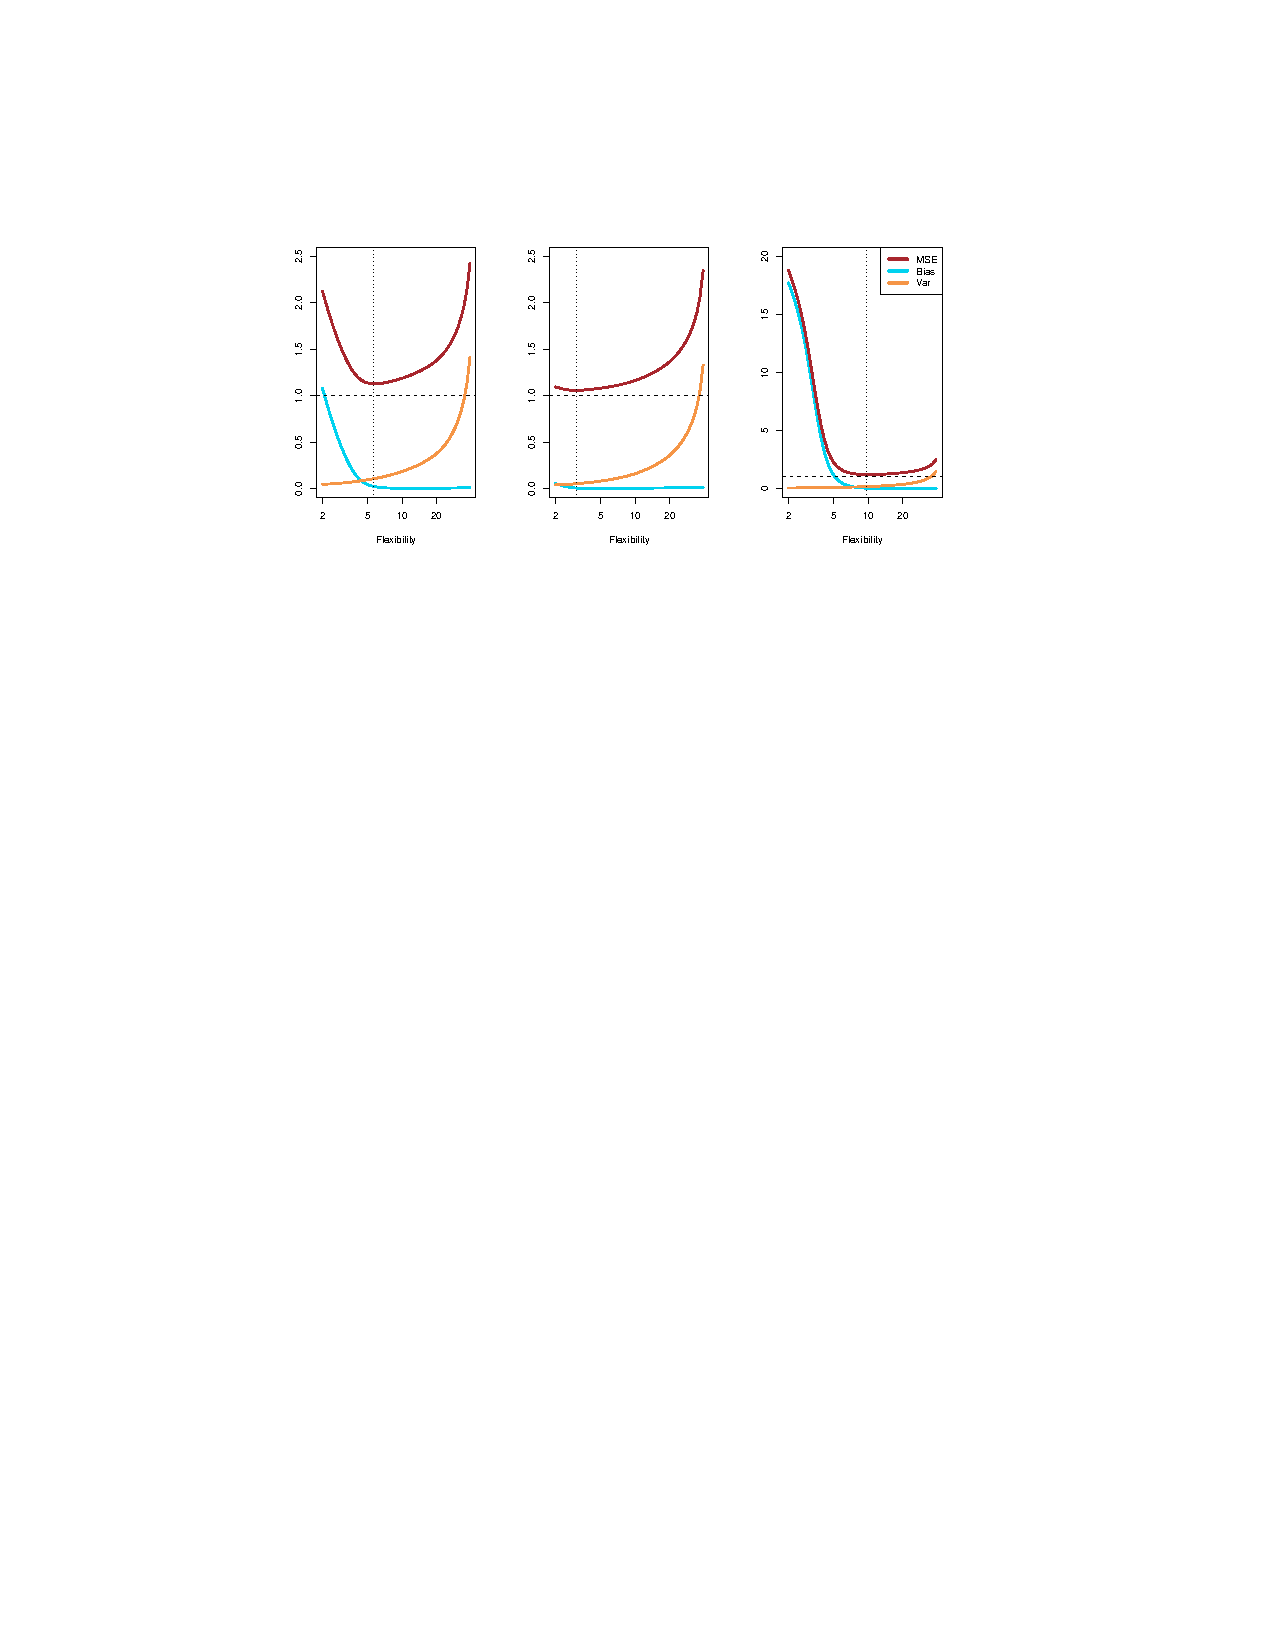
\includegraphics[width=\textwidth]{img/the-bias-variance-trade-off-1.pdf}
                \captionof{figure}{Squared bias (blue curve), variance (orange curve), $\Var\left(\varepsilon\right)$ (dashed line), and test MSE (red curve) for the three data sets in Figures \ref{fig: measuring the quality of fit}, \ref{fig: measuring the quality of fit - 2}, \ref{fig: measuring the quality of fit - 3}. The vertical dotted line indicates the flexibility level corresponding to the smallest test MSE.\cite{james2013introduction}}
                \label{fig: the bias-variance trade-off}
            \end{center}

            Three plots illustrate equation~\ref{eq: expected test MSE} on page~\pageref{eq: expected test MSE} for the examples in Figure \ref{fig: measuring the quality of fit}, \ref{fig: measuring the quality of fit - 2}, \ref{fig: measuring the quality of fit - 3}.

            In each case the blue solid curve represents the squared bias, for different levels of flexibility, while the orange curve corresponds to the variance. The horizontal dashed line represents $\Var\left(\varepsilon\right)$, the irreducible error. Finally, the red curve, corresponding to the test set MSE, is the sum of these three quantities. 
            
            \highspace
            In all three cases, the variance increases and the bias decreases as the method's flexibility increases. However, the flexibility level corresponding to the optimal test MSE differs considerably among the three data sets, because the squared bias and variance change at different rates in each of the data sets. 
            
            \highspace
            In the left-hand panel of this Figure, the bias initially decreases rapidly, resulting in an initial sharp decrease in the expected test MSE. 
            
            \highspace
            On the other hand, in the center panel of this Figure the true $f$ is close to linear, so there is only a small decrease in bias as flexibility increases, and the test MSE only declines slightly before increasing rapidly as the variance increases. 
            
            \highspace
            Finally, in the right-hand panel of this Figure, as flexibility increases, there is a dramatic decline in bias because the true $f$ is very non-linear. There is also very little increase in variance as flexibility increases. Consequently, the test MSE declines substantially before experiencing a small increase as model flexibility increases.
        \end{examplebox}
    \end{figure}

    \newpage

    \begin{flushleft}
        \textcolor{Red2}{\faIcon[regular]{star} \textbf{Meaning of the bias-variance trade-off}}
    \end{flushleft}
    The relationship between bias, variance, and test set MSE given in equation~\ref{eq: expected test MSE} on page~\pageref{eq: expected test MSE} and displayed in the Figure~\ref{fig: the bias-variance trade-off} (previous example) is referred to as the \definition{bias-variance trade-off}. 
    
    \highspace
    Good test set performance of a statistical learning method requires low variance as well as low squared bias. This is referred to as a \textbf{trade-off} because it is \textbf{easy to obtain a method with extremely low bias but high variance}\footnote{For \example{instance}, by drawing a curve that passes through every single training observation} or \textbf{a method with very low variance but high bias} (by fitting a horizontal line to the data).
    
    \highspace
    The \textbf{challenge lies in finding a method for which both the variance and the squared bias are low}. This trade-off is one of the most important recurring themes in this course.

    \newpage

    \subsection{Algorithm: K-Nearest Neighbors (KNN)}

    Many approaches attempt to \textbf{estimate the conditional distribution of} $\bm{Y}$ \textbf{given} $\bm{X}$, and \textbf{then classify a given observation to the class} with \textbf{highest estimated probability}. One such method is the \definition{K-nearest neighbors (KNN)} classifier.

    \highspace
    In mathematical terms, given a positive integer $K$ and a test observation $x_{0}$ the KNN classifier:
    \begin{enumerate}
        \item \textbf{Identifies} the $K$ points in the training data that are closest to $x_{0}$, represented by $\mathcal{N}_{0}$.
        
        \item It then \textbf{estimates} the conditional probability for class $j$ as the fraction of points in $\mathcal{N}_{0}$ whose response values equal $j$:
        \begin{equation}\label{eq: KNN}
            \Pr\left(Y=J \: | \: X=x_{0}\right) = \dfrac{1}{K} \displaystyle\sum_{i \in \mathcal{N}_{0}} I\left(y_{i} = j\right)
        \end{equation}

        \item Finally, KNN \textbf{classifies} the test observation $x_{0}$ to the class with the largest probability from the previous equation.
    \end{enumerate}
    
    \begin{examplebox}
        Suppose that we choose $K=3$. Then KNN algorithm:
        \begin{enumerate}
            \item Identify the three observations that are closet to the cross. As you can see in the Figure~\ref{fig: KNN} on page~\pageref{fig: KNN}, this neighborhood is shown as a circle. It consists of two blue points and one orange point, resulting in estimated probabilities of $\dfrac{2}{3}$ for the blue class and $\dfrac{1}{3}$ for the orange class.
            
            \item Hence, KNN will predict that the black cross belongs to the blue class.
        \end{enumerate}
    \end{examplebox}

    \newpage

    \begin{figure}[!htp]
        \begin{examplebox}
            \begin{center}
                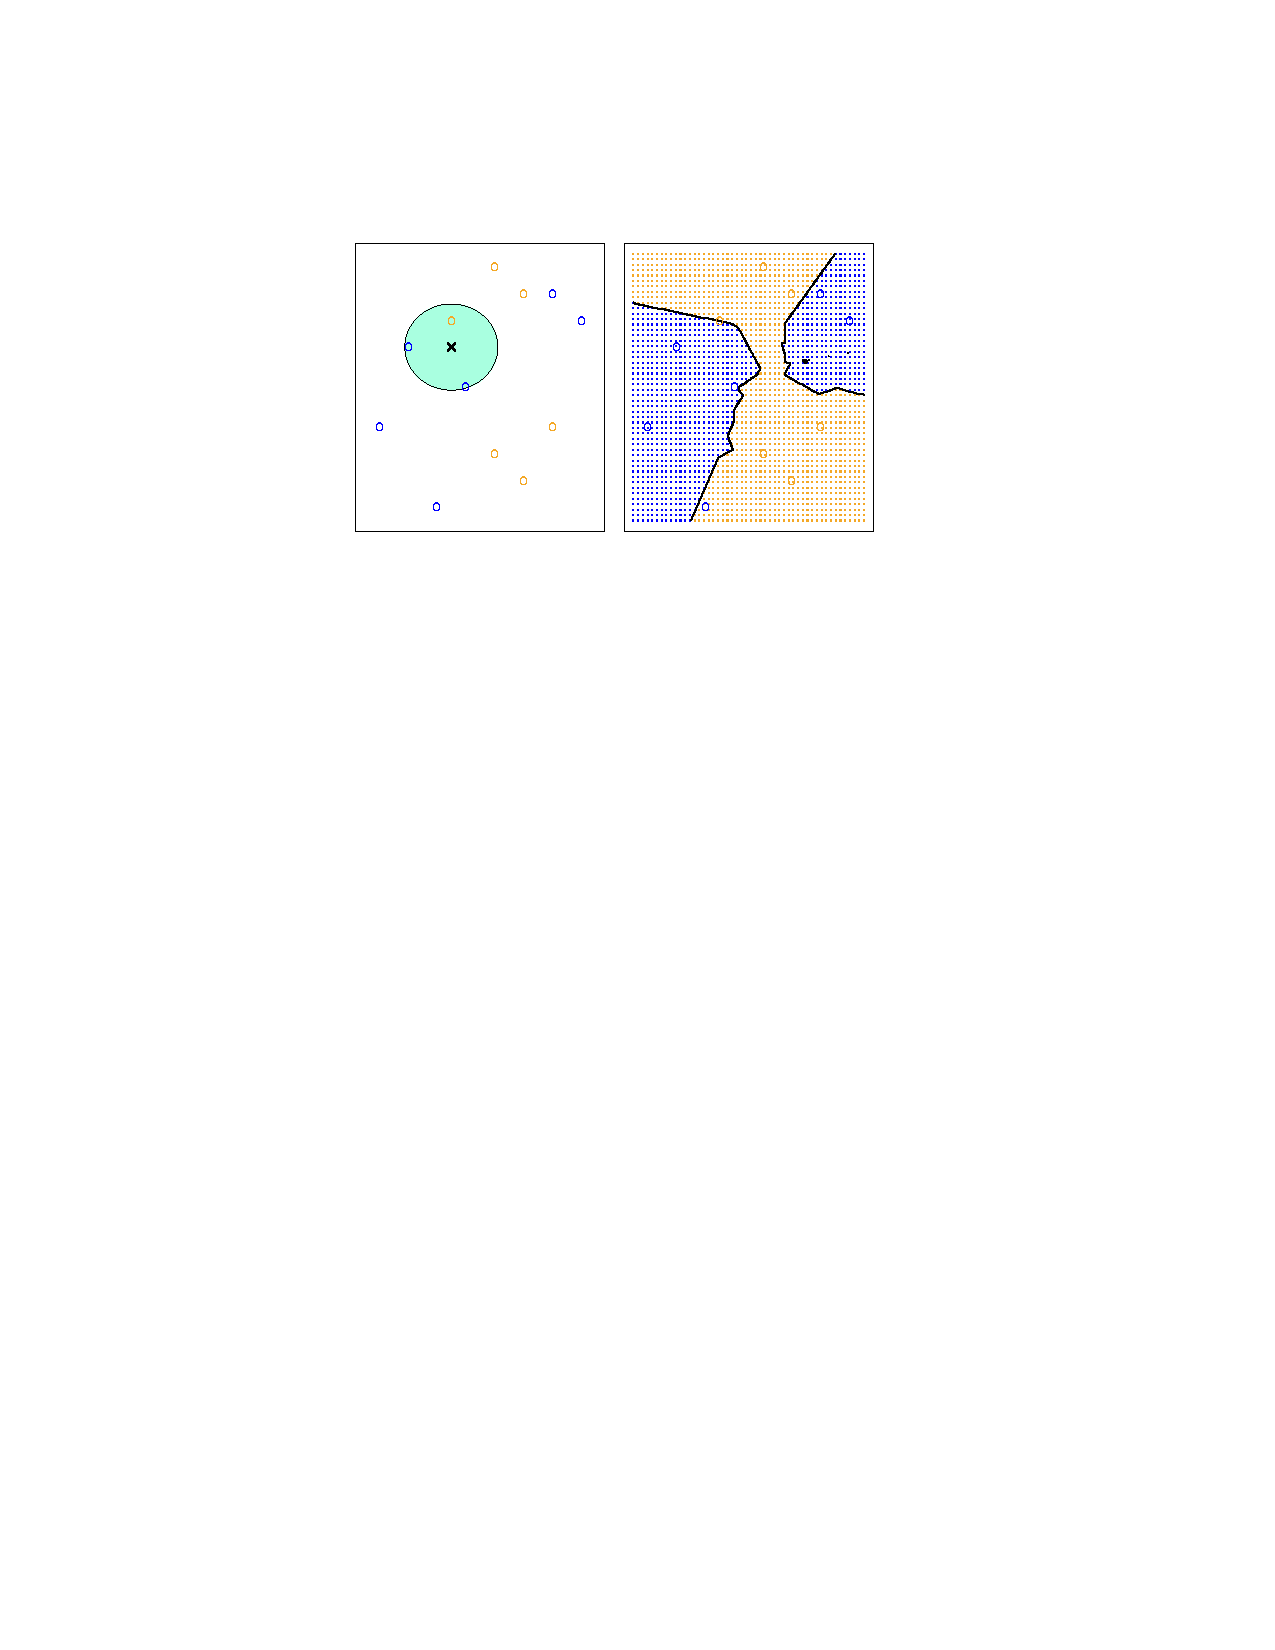
\includegraphics[width=\textwidth]{img/KNN-1.pdf}
                \captionof{figure}{The KNN approach, using $K=3$, is illustrated in a simple situation with six blue observations and six orange observations. Left: \emph{a test observation at which a predicted class label is desired is shown as a black cross. The three closest points to the test observation are identified, and it is predicted that the test observation belongs to the most commonly-occurring class, in this case blue}. Right: \emph{the KNN decision boundary for this example is shown in black. The blue grid indicates the region in which a test observation will be assigned to the blue class, and the orange grid indicates the region in which it will be assigned to the orange class}.}
                \label{fig: KNN}
            \end{center}

            This figure provides an illustrative example of the KNN approach. In the left-hand panel, we have plotted a small training data set consisting of six blue and six orange observations. Our goal is to make a prediction for the point labeled by the black cross.

            \highspace
            In the right-hand panel, we have applied the KNN approach with $K=3$ at all of the possible values for $X_{1}$ and $X_{2}$, and have drawn in the corresponding KNN decision boundary.
        \end{examplebox}
    \end{figure}

    \newpage

    \begin{figure}[!htp]
        \begin{examplebox}
            \begin{center}
                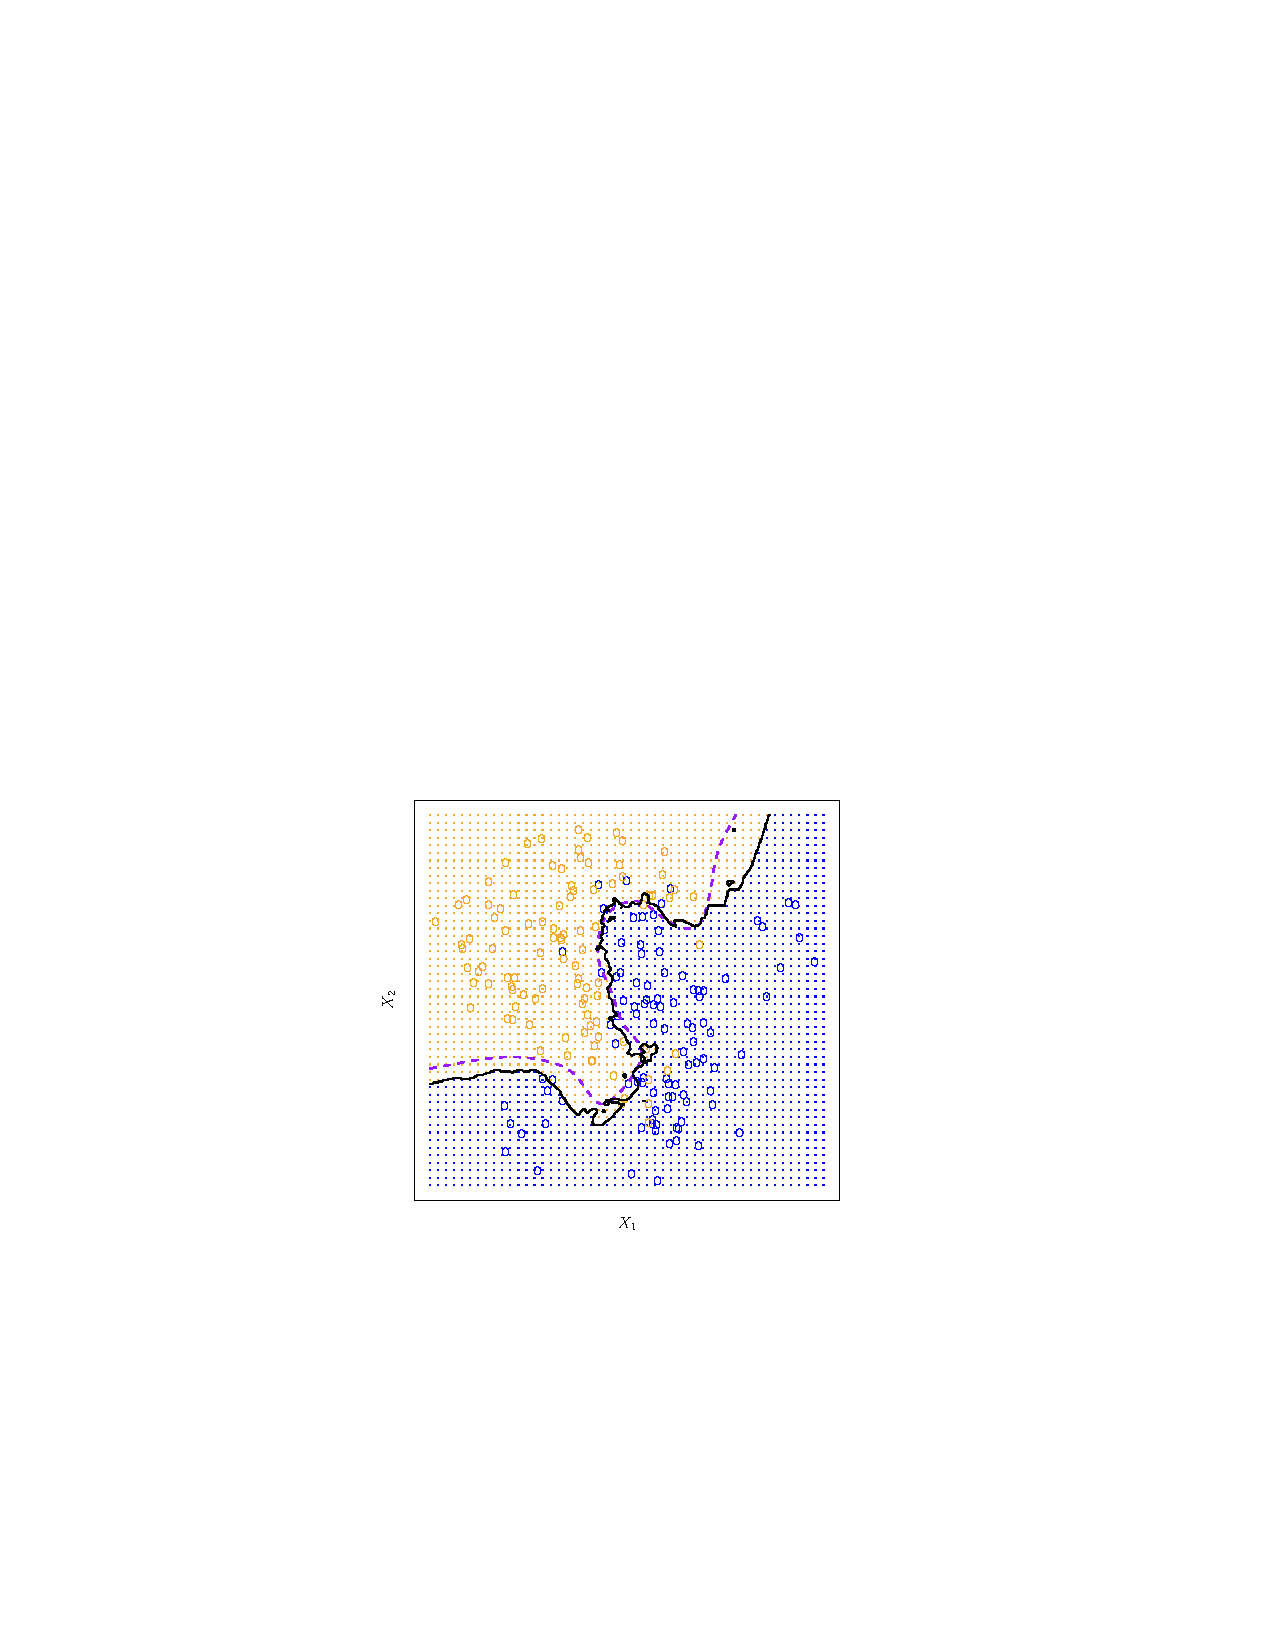
\includegraphics[width=\textwidth]{img/KNN-2.pdf}
                \captionof{figure}{The black curve indicates the KNN decision boundary on the data, using $K=10$. The Bayes decision boundary is shown as a purple dashed line. The KNN and Bayes decision boundaries are very similar.}
                \label{fig: KNN 2}
            \end{center}

            This Figure displays the KNN decision boundary, using $K=10$, when applied to the larger simulated data set.
        \end{examplebox}
    \end{figure}


















    %%%%%%%%%%%%%%%%%%%%%%%%%%%%%%%%%%%%%%%%%%%%%%%%%%%%%%%%%%%%%%%%%%%%%%%%%%%%%%%%%%%%%%%%
    %%%%%%%%%%%%%%%%%%%%%%%%%%%%%%%%%%%%%% Laboratory %%%%%%%%%%%%%%%%%%%%%%%%%%%%%%%%%%%%%%
    %%%%%%%%%%%%%%%%%%%%%%%%%%%%%%%%%%%%%%%%%%%%%%%%%%%%%%%%%%%%%%%%%%%%%%%%%%%%%%%%%%%%%%%%

    \newpage

    \section{R language programming}

    \subsection{Introduction to R}

    There is no introduction to RStudio in these notes. But you can find a detailed guide \href{https://moderndive.netlify.app/1-getting-started#getting-started}{here}.

    \highspace
    \texttt{R} uses functions to perform operations. To run a function called \texttt{funcname}, we type \texttt{funcname(input1, input2)}, where the inputs (or arguments) \texttt{input1} and \texttt{input2} tell \texttt{R} how to run the function.

    \newpage

    \subsubsection{Scalars, vectors and matrices}

    \begin{itemize}
        \item Create a \textbf{scalar}
        \lstinputlisting[language=R]{code/scalars-1.r}

        \item Create a \textbf{vector}
        \lstinputlisting[language=R]{code/vectors-1.r}
        And the result is always the same:
        \lstinputlisting{code/output-vectors-1}
        \begin{itemize}
            \item \texttt{c} function (\href{https://www.rdocumentation.org/packages/base/versions/3.6.2/topics/c}{documentation}) takes $n$ arguments to create a vector of length $n$.

            \item \texttt{seq} function (\href{https://www.rdocumentation.org/packages/base/versions/3.6.2/topics/seq}{doc}) takes two arguments to create a vector with these two values as its lower and upper bound. In the example code, the values are passed implicitly, but we can make them explicit with \texttt{from} and \texttt{to}:
            \lstinputlisting[language=R]{code/vectors-2.r}
            And the result is always the same:
            \lstinputlisting{code/output-vectors-1}
            The \texttt{len} parameter specifies the length of the vector. For example:
            \lstinputlisting[language=R]{code/vectors-3.r}
            And the result is:
            \lstinputlisting{code/output-vectors-3}
            With the \texttt{by} argument, we can increment the sequence:
            \lstinputlisting[language=R]{code/vectors-4.r}
            And the result is:
            \lstinputlisting{code/output-vectors-4}

            \item The \texttt{:} (colon operator, \href{https://www.rdocumentation.org/packages/base/versions/3.6.2/topics/Colon}{doc}) generates a regular sequence. It's very easy to use: \texttt{from:to}.
        \end{itemize}

        \item Create a \textbf{matrix}
        \lstinputlisting[language=R]{code/matrices-1.r}
        And the result is always the same:
        \lstinputlisting{code/output-matrices-1}
        \begin{itemize}
            \item The \texttt{rbind} and \texttt{cbind} (\href{https://www.rdocumentation.org/packages/base/versions/3.6.2/topics/cbind}{doc}) functions are very similar. Both take a sequence of vector, matrix or data-frame arguments and combine by rows or columns, respectively. So if we use \texttt{rbind}, we need to specify the lines. If we use \texttt{cbind} instead, we need to specify each column.
            
            A useful piece of advice when using \texttt{rbind} or \texttt{cbind} is the code style. The following code is easier to read:
            \lstinputlisting[language=R]{code/matrices-2.r}
            We can also convert a vector into a row vector with \texttt{rbind} or a column vector with \texttt{cbind}.

            \item The \texttt{matrix} (\href{https://www.rdocumentation.org/packages/base/versions/3.6.2/topics/matrix}{doc}) function creates a matrix from the given set of values. The arguments:
            \begin{itemize}
                \item \texttt{data} is an optional data vector.
                \item \texttt{nrow} is the desired number of rows.
                \item \texttt{ncol} is the desired number of columns.
                \item \texttt{byrow} is a logical argument. If \texttt{FALSE} (or \texttt{F}, the default) the matrix is filled by columns, otherwise the matrix is filled by rows.
            \end{itemize}
            \lstinputlisting[language=R]{code/matrices-3.r}
        \end{itemize}
    \end{itemize}

    \subsubsection{Access elements}

    We can access to an \textbf{element of a vector} using the square brackets.
    \begin{itemize}
        \item By explicitly inserting the index
        \lstinputlisting[language=R]{code/access-elements-1.r}

        \item By explicitly inserting a vector as an index to access multiple elements
        \lstinputlisting[language=R]{code/access-elements-2.r}

        \item By explicitly inserting a negative value as an index to access all values except the specified index value (is the opposite of a positive index value)
        \lstinputlisting[language=R]{code/access-elements-3.r}

        \item By explicitly inserting a negative vector as an index to access all values except the specified vector value (is the opposite of a positive vector value)
        \lstinputlisting[language=R]{code/access-elements-4.r}
    \end{itemize}
    We can access to an \textbf{element of a matrix} using the square brackets.
    \begin{itemize}
        \item By explicitly inserting the index
        \lstinputlisting[language=R]{code/access-elements-5.r}

        \item By explicitly inserting a vector as an index (column or row) to access multiple elements
        \lstinputlisting[language=R]{code/access-elements-6.r}

        \item By explicitly inserting a blank to access all values of the row/column
        \lstinputlisting[language=R]{code/access-elements-7.r}
    \end{itemize}

    \newpage

    \subsubsection{Algebraic operations}

    By default, operations in \texttt{R} are performed on a component-by-component basis. For example, given the following data:
    \lstinputlisting[language=R, firstline=1, lastline=7]{code/algebraic-operations-1.r}
    Operations with the \textbf{vectors}:
    \begin{itemize}
        \item \textbf{Sum} between two scalars
        \lstinputlisting[language=R, firstline=9, lastline=10]{code/algebraic-operations-1.r}

        \item \textbf{Sum} between two vectors
        \lstinputlisting[language=R, firstline=11, lastline=12]{code/algebraic-operations-1.r}

        \item \textbf{Sum} between a vector and a scalar
        \lstinputlisting[language=R, firstline=17, lastline=18]{code/algebraic-operations-1.r}

        \item \textbf{Sums} the components of a vector
        \lstinputlisting[language=R, firstline=23, lastline=24]{code/algebraic-operations-1.r}

        \item \textbf{Multiply} between two scalars
        \lstinputlisting[language=R, firstline=13, lastline=14]{code/algebraic-operations-1.r}

        \item \textbf{Multiply} between two vectors
        \lstinputlisting[language=R, firstline=15, lastline=16]{code/algebraic-operations-1.r}

        \item \textbf{Multiplies} between the components of a vector
        \lstinputlisting[language=R, firstline=25, lastline=26]{code/algebraic-operations-1.r}

        \item \textbf{Exponential} of a vector
        \lstinputlisting[language=R, firstline=19, lastline=20]{code/algebraic-operations-1.r}

        \item \textbf{Exponential function} of a vector
        \lstinputlisting[language=R, firstline=21, lastline=22]{code/algebraic-operations-1.r}
    \end{itemize}

    \newpage

    \noindent
    Operations with the \textbf{matrices}. Given the following data:
    \lstinputlisting[language=R, firstline=1, lastline=4]{code/algebraic-operations-2.r}
    \begin{itemize}
        \item \textbf{Transpose} of a matrix
        \lstinputlisting[language=R, firstline=6, lastline=10]{code/algebraic-operations-2.r}

        \item \textbf{Inverse} of a matrix
        \lstinputlisting[language=R, firstline=47, lastline=50]{code/algebraic-operations-2.r}

        \item \textbf{Determinant} of a matrix
        \lstinputlisting[language=R, firstline=52, lastline=53]{code/algebraic-operations-2.r}

        \item The generic function \textbf{solves} the equation \texttt{a \%*\% x = b} for \texttt{x}, where \texttt{b} can be either a vector or a matrix. If \texttt{b} is missing, it's taken to be an identity matrix and \texttt{solve} will return the inverse of \texttt{a}.
        \lstinputlisting[language=R, firstline=55, lastline=63]{code/algebraic-operations-2.r}

        \item \textbf{Sum} between matrices
        \lstinputlisting[language=R, firstline=12, lastline=15]{code/algebraic-operations-2.r}

        \item \textbf{Sum} between matrices and scalars
        \lstinputlisting[language=R, firstline=36, lastline=39]{code/algebraic-operations-2.r}

        \item \textbf{Sum} between matrices and vectors
        \lstinputlisting[language=R, firstline=41, lastline=44]{code/algebraic-operations-2.r}

        \item \textbf{Multiplication} (component-by-component) between matrices
        \lstinputlisting[language=R, firstline=17, lastline=20]{code/algebraic-operations-2.r}

        \item \textbf{Multiplication} (classic) between matrices
        \lstinputlisting[language=R, firstline=22, lastline=34]{code/algebraic-operations-2.r}
    \end{itemize}

    \newpage

    \subsubsection{Categorical data}

    The function \texttt{factor} is used to encode a vector as a factor. Arguments:
    \begin{itemize}
        \item \texttt{x}: a vector of data, usually taking a small number of distinct values.
        \item \texttt{levels}: an optional vector of the unique values (as character strings) that \texttt{x} might have taken.
    \end{itemize}
    For example:
    \lstinputlisting[language=R]{code/categorical-data-1.r}
    The function \texttt{table} uses cross-classifying factors to build a contingency table of the counts at each combination of factor levels.
    \lstinputlisting[language=R]{code/categorical-data-2.r}

    \newpage

    \subsubsection{Lists}

    A \texttt{list} in \texttt{R} is a generic object consisting of an \textbf{ordered collection of objects}. Lists are one-dimensional, heterogeneous data structures. The list can be a list of vectors, a list of matrices, a list of characters and a list of functions, and so on.

    \highspace
    For example, here is a \texttt{list} containing the results of an exam:
    \lstinputlisting[language=R, firstline=1, lastline=28]{code/lists-1.r}
    To access a property of the object, we can use the \$ symbol or the square brackets:
    \lstinputlisting[language=R, firstline=30, lastline=34]{code/lists-1.r}

    \newpage

    \subsubsection{Data Frames}

    The function \texttt{data.frame()} creates data frames, tightly coupled collections of variables which share many of the properties of matrices and of lists, used as the fundamental data structure by most of \texttt{R}'s modeling software.

    \highspace
    For example:
    \lstinputlisting[language=R, firstline=1, lastline=21]{code/data-frames.1.r}
    Like the lists, to access a property of the data frame, we can use \$, or the square brackets:
    \lstinputlisting[language=R, firstline=23, lastline=30]{code/data-frames.1.r}
    The data frame has two important and frequently used functions: \texttt{attach} and \texttt{detach}:
    \begin{itemize}
        \item In R, \texttt{attach()} is a function that allows us to attach a database (usually a \texttt{data frame}) to the \texttt{R} search path. This function makes it easier to interact with objects within \texttt{data frame}s by eliminating the need to repeatedly reference the data frame itself.

        In simpler terms, the \texttt{attach()} function takes a data frame and places it in the search path of R's environment. Once a data frame is attached, we can \textbf{call its variables directly, without the need to use the \$ operator or square brackets}.
        \lstinputlisting[language=R, firstline=32, lastline=36]{code/data-frames.1.r}

        \item The \texttt{detach()} function detaches a database. Usually this is either a \texttt{data.frame} which has been attached or a package which was attached by library.
        \lstinputlisting[language=R, firstline=38, lastline=40]{code/data-frames.1.r}
    \end{itemize}

    \newpage

    \subsubsection{Reading and writing data}

    The \texttt{read.table} function reads a file in table format and creates a data frame from it, with cases corresponding to lines and variables to fields in the file. It can also read a csv file. It has the following (not all) parameters:
    \begin{itemize}
        \item \texttt{file}: \textbf{the name of the file which the data are to be read from}. Each row of the table appears as one line of the file. If it does not contain an absolute path, the file name is relative to the current working directory, \texttt{getwd()}. 
        
        For example, if our working directory is 
        \begin{center}
            \texttt{C:\textbackslash Users\textbackslash Applied-Statistics}
        \end{center}
        and we have a folder \texttt{1-lesson} within the working directory, to access a file within the folder we can write the absolute path:
        \begin{center}
            \texttt{C:\textbackslash Users\textbackslash Applied-Statistics\textbackslash 1-lesson\textbackslash file-name.txt}
        \end{center}
        or the relative path \texttt{1-lesson\textbackslash file-name.txt}.

        \item \texttt{header}: a logical value indicating whether the file contains the names of the variables as its first line. If missing, the value is determined from the file format: \textbf{header is set to \texttt{TRUE} if and only if the first row contains one fewer field than the number of columns}.
    \end{itemize}
    For example, given the following raw (txt) file:\label{code: read.table - raw file}
    \lstinputlisting{code/record.txt}
    The \texttt{R} code to read it is:
    \lstinputlisting[language=R, firstline=1, lastline=1]{code/reading-and-writing-data-1.r}
    Some useful functions:
    \begin{itemize}
        \item \texttt{head} or \texttt{tail}: Returns the first or last parts of a vector, matrix, table, data frame or function.
        \lstinputlisting[language=R, firstline=3, lastline=10]{code/reading-and-writing-data-1.r}

        \item \texttt{dim}: Retrieve or set the dimension of an object.
        \begin{itemize}
            \item For \texttt{data.frame} returns the lengths of the \texttt{row.names} attribute of \texttt{x} and of \texttt{x} (as the numbers of rows and columns respectively).

            \item For an \texttt{array} (and hence in particular, for a \texttt{matrix}) \texttt{dim} retrieves the \texttt{dim} attribute of the object.
        \end{itemize}
        In the previous example, the number of rows, excluding the header, is 55 and the number of columns is 7:
        \lstinputlisting[language=R, firstline=12, lastline=13]{code/reading-and-writing-data-1.r}

        \newpage

        \item \texttt{dimnames}: Retrieve or set the \texttt{dimnames} of an object. The \texttt{dimnames} of a \texttt{data frame} are its \texttt{row.names} and its \texttt{names}.
        \lstinputlisting[language=R, firstline=15, lastline=25]{code/reading-and-writing-data-1.r}
    \end{itemize}
    To serialize (\dquotes{save}) a specific object or an entire workspace, we can use:
    \begin{itemize}
        \item \texttt{save} writes an external representation of \texttt{R} objects to the specified file. The objects can be read back from the file at a later date by using the function \texttt{load} or \texttt{attach} (or \texttt{data} in some cases).
        
        \item \texttt{save.image} is short-cut for \dquotes{save my current workspace}.

        \item \texttt{load}: Reload datasets written with the function \texttt{save}.
    \end{itemize}
    \textbf{Note: the extension of the serialization file must be \texttt{.RData}}
    \lstinputlisting[language=R]{code/reading-and-writing-data-2.r}
    We can also use the \texttt{ls} and \texttt{rm} combination to clean up the entire workspace:
    \begin{itemize}
        \item \texttt{ls} returns a vector of character strings giving the names of the objects in the specified environment. When invoked with no argument at the top level prompt, \texttt{ls} shows what data sets and functions a user has defined. When invoked with no argument inside a function, \texttt{ls} returns the names of the function's local variables.

        \item \texttt{rm} can be used to remove objects.
    \end{itemize}
    \lstinputlisting[language=R]{code/reading-and-writing-data-3.r}

    \newpage

    \subsubsection{Example: analysis of quantitative data}

    Given the raw file on page~\pageref{code: read.table - raw file}, we convert the values of the last 4 columns into seconds. Then we load it:\label{code: read.table - modded}
    \lstinputlisting[language=R, firstline=1, lastline=65]{code/example-analysis-of-quantitative-data-1.r}
    Now we want to calculate: the means of each column (we will show two methods); the standard deviation; the variance; the covariance.
    \begin{itemize}
        \item \texttt{colMeans}: Form row and column sums and means for numeric arrays (or data frames).

        \item \texttt{apply}: Returns a list of the same length as \texttt{X} (input parameter), each element of which is the result of applying \texttt{FUN} (function, e.g. \texttt{mean}, \texttt{var}, etc.) to the corresponding element of \texttt{X}.

        \item \texttt{mean}: Arithmetic mean.

        \item \texttt{sd}: This function computes the standard deviation of the values in \texttt{x} (input parameter). If \texttt{na.rm} is \texttt{TRUE} then missing values are removed before computation proceeds.
        
        \item \texttt{var}: Computes the variance.
        
        \item \texttt{cov}: Computes the covariance.
        
        \item \texttt{cor}: Computes the correlation.
    \end{itemize}
    \lstinputlisting[language=R, firstline=67, lastline=73]{code/example-analysis-of-quantitative-data-1.r}
    And the result is on the following page.

    \newpage

    \begin{figure}[!htp]
        \centering
        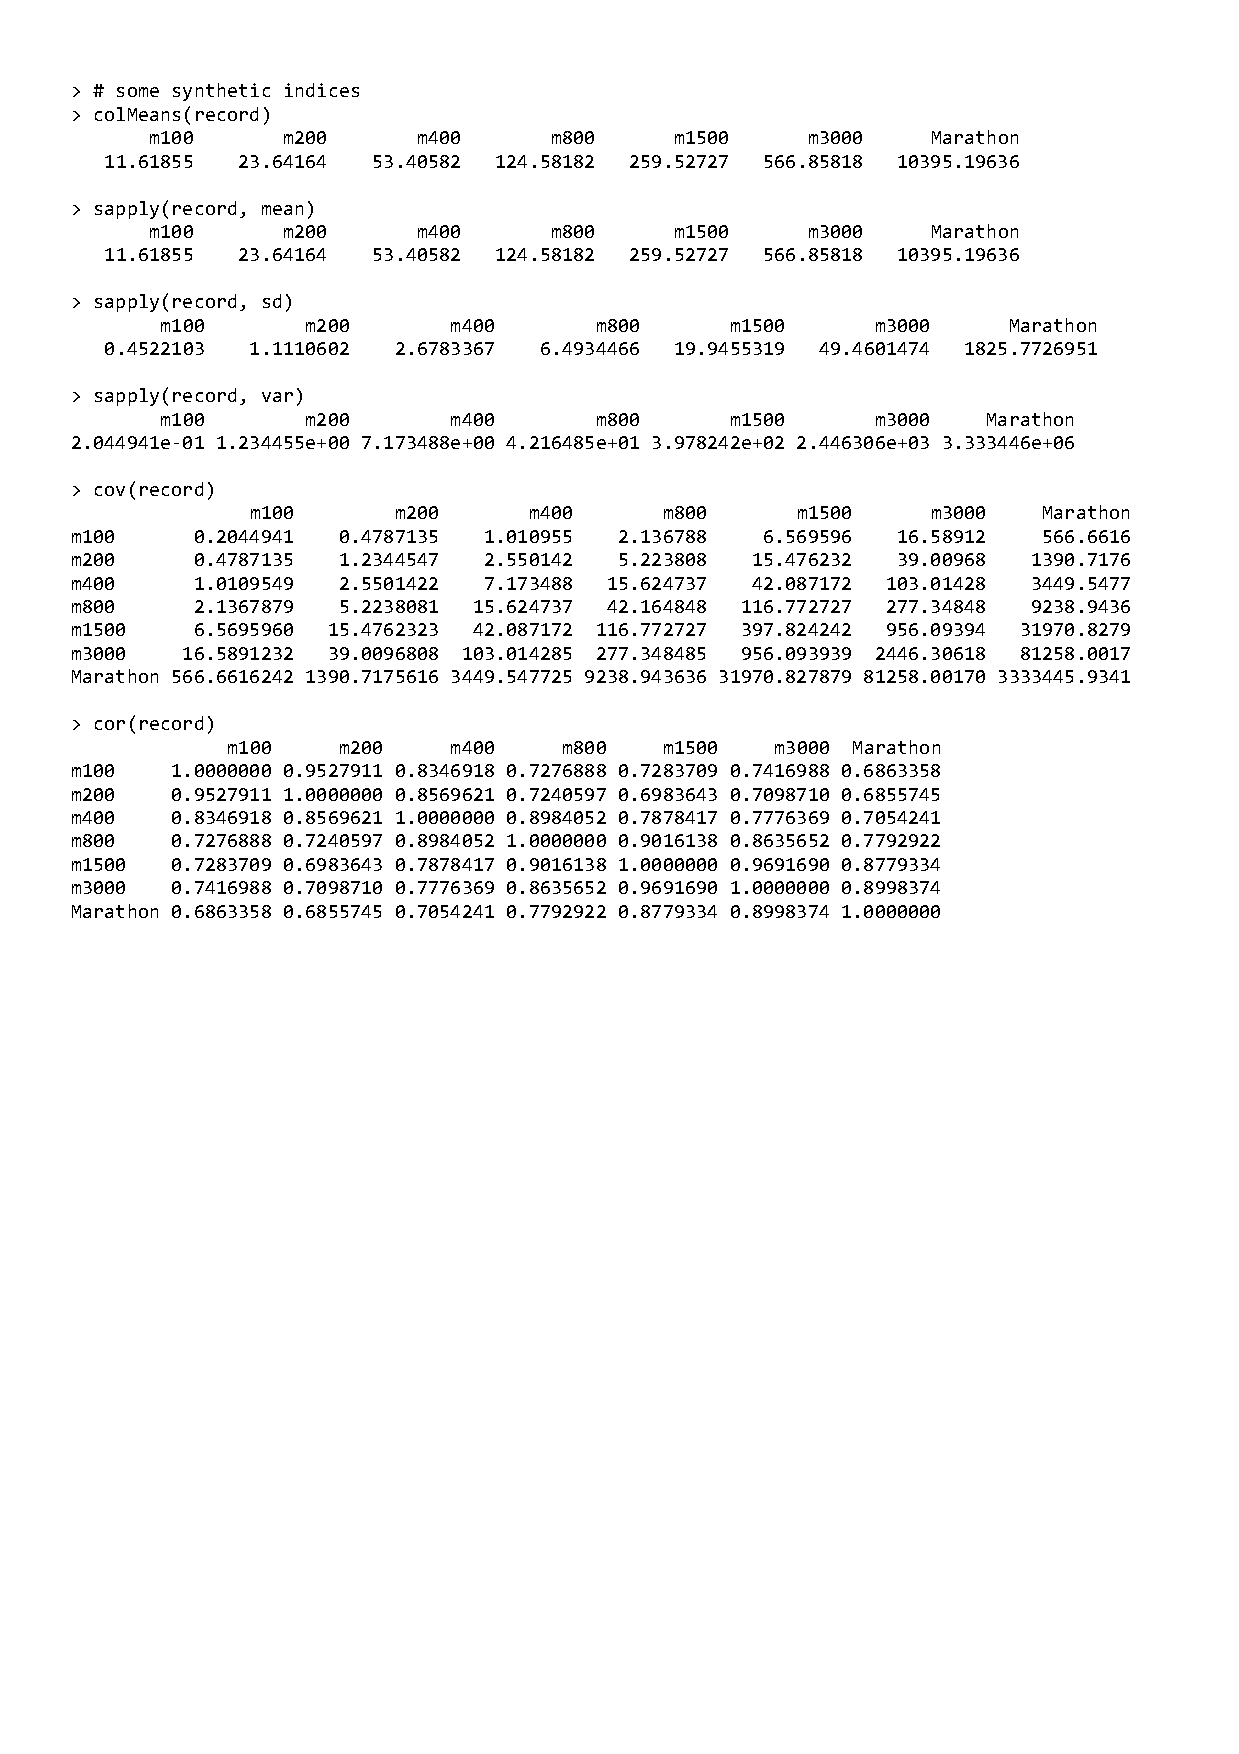
\includegraphics[width=\textwidth]{img/example-analysis-of-quantitative-data-1.pdf}
    \end{figure}

    \newpage

    \begin{flushleft}
        \large
        \textbf{Univariate t-test for the mean value of the quantity}
    \end{flushleft}
    We print a quantile-quantile plot\footnote{In statistics, a Q-Q plot (quantile-quantile plot) is a probability plot, a graphical method for comparing two probability distributions by plotting their quantiles against each other.\cite{10.1093/biomet/55.1.1}} (\texttt{qqplot}) to verify (qualitatively) the Gaussian assumption on the distribution generating sample.
    \begin{itemize}
        \item \texttt{qqnorm} is a generic function the default method of which produces a normal QQ plot of the values in \texttt{y} (input parameter).
        
        \item \texttt{qqline} adds a line to a \dquotes{theoretical}, by default normal, quantile-quantile plot which passes through the probs quantiles, by default the first and third quartiles.
    \end{itemize}
    \lstinputlisting[language=R, firstline=75, lastline=76]{code/example-analysis-of-quantitative-data-1.r}
    \begin{figure}[!htp]
        \centering
        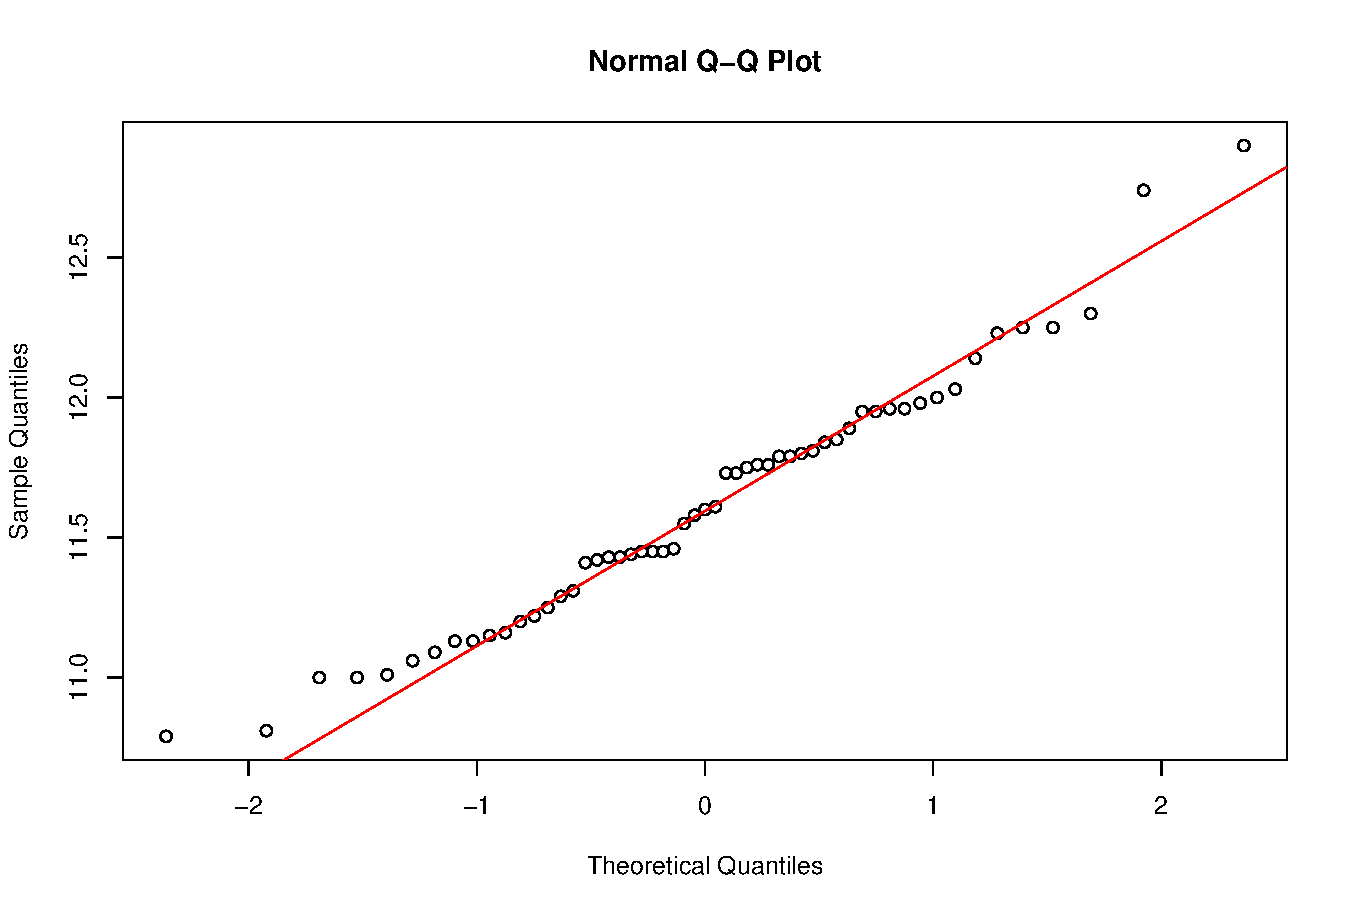
\includegraphics[width=\textwidth]{img/example-analysis-of-quantitative-data-2.pdf}
    \end{figure}
    
    \noindent
    Furthermore, we use Shapiro-Wilk test\footnote{The Shapiro-Wilk test is a test of normality. In statistics, normality tests are used to determine if a data set is well-modeled by a normal distribution and to compute how likely it is for a random variable underlying the data set to be normally distributed (\href{https://en.wikipedia.org/wiki/Normality_test}{source}).} to verify (quantitatively) the Gaussian assumption on the distribution generating sample.
    \lstinputlisting[language=R, firstline=78, lastline=82]{code/example-analysis-of-quantitative-data-1.r}
    \begin{itemize}
        \item \texttt{W}: the value of the Shapiro-Wilk statistic.
        \item \texttt{p.value}: an approximate p-value for the test. This is said in Royston (1995) to be adequate for \texttt{p.value < 0.1}.
        \item \texttt{data.name}: a character string giving the name(s) of the data.
    \end{itemize}

    \newpage

    \noindent
    The null-hypothesis of this test is that the population is normally distributed. Thus, if:
    \begin{itemize}
        \item The \texttt{p.value} is \textbf{less than the chosen} \texttt{alpha} level, then the null hypothesis is \textbf{rejected} and there is evidence that the data tested are \underline{not} normally distributed.

        \item The \texttt{p.value} is \textbf{greater than the chosen} \texttt{alpha} level, then the null hypothesis (that the data came from a normally distributed population) can \underline{not} be rejected.
    \end{itemize}
    So in our case the data is normally distributed because the alpha level is 0.05.

    \highspace
    Now, we perform the Student's t-Test\footnote{Student's t-Test is a statistical test used to test whether the difference between the response of two groups is statistically significant or not. A \textbf{one-sample} Student's t-test is a location test of whether the mean of a population has a value specified in a null hypothesis. In testing the null hypothesis that the population mean is equal to a specified value $\mu_{0}$, one uses the statistic:
    \begin{equation*}
        t = \dfrac{\overline{x}-\mu_{0}}{s \div \sqrt{n}}
    \end{equation*}
    Where $\overline{x}$ is the sample mean, $s$ is the sample standard deviation and $n$ is the sample size. The degrees of freedom used in this test are $n-1$. Although the parent population does not need to be normally distributed, the distribution of the population of sample means $\overline{x}$ is assumed to be normal.}. The arguments:
    \begin{itemize}
        \item \texttt{x} a non-empty numeric vector of data values.
        
        \item \texttt{alternative} a character string specifying the alternative hypothesis, must be one of "\texttt{two.sided}" (default), "\texttt{greater}" or "\texttt{less}"

        \item \texttt{mu} a number indicating the true value of the mean (or difference in means if you are performing a two sample test).
        
        \item \texttt{conf.level} confidence level of the interval.
    \end{itemize}
    The output values:
    \begin{itemize}
        \item \texttt{t}: the value of the t-test.

        \item \texttt{df}: the degrees of freedom for the t-test.

        \item \texttt{p-value}: the p-value for the test.

        \item \texttt{confidence interval}: a confidence interval for the mean appropriate to the specified alternative hypothesis.

        \item \texttt{estimate}: the estimated mean or difference in means depending on whether it was a one-sample test or a two-sample test.
    \end{itemize}
    See the code in the following page.

    \newpage
    
    \lstinputlisting[language=R, firstline=84, lastline=98]{code/example-analysis-of-quantitative-data-1.r}
    We can also run the Student's t-test manually:
    \lstinputlisting[language=R, firstline=100, lastline=117]{code/example-analysis-of-quantitative-data-1.r}

    \newpage

    \begin{flushleft}
        \large
        \textbf{Simple linear regression}
    \end{flushleft}
    We want to calculate the simple linear regression\footnote{In statistics, simple linear regression (SLR) is a linear regression model with a single explanatory variable. That is, it concerns two-dimensional sample points with one independent variable and one dependent variable (conventionally, the $x$ and $y$ coordinates in a Cartesian coordinate system) and finds a linear function (a non-vertical straight line) that, as accurately as possible, predicts the dependent variable values as a function of the independent variable. The adjective simple refers to the fact that the outcome variable is related to a single predictor.} of the property \texttt{m100} and of the property \texttt{m200}. We then want to create a scatter plot to see the graphical relationship between these two sets of data. We will also create a linear model to calculate the true linear regression.

    \highspace
    In this section, \texttt{m100} e \texttt{m200} are properties of the \texttt{record} object created on page~\pageref{code: read.table - modded}.

    \highspace
    First, we plot \texttt{m100} and \texttt{m200} using:
    \begin{itemize}
        \item \texttt{par}: prepares the graphical environment. It is a powerful tool and in this case it is used to create a $2 \times 2$ matrix so that each graph can be placed in just one figure. It's also possible to use the \texttt{layout} function.

        \item \texttt{hist}: The generic function \texttt{hist} computes a histogram of the given data values. With the arguments:
        \begin{itemize}
            \item \texttt{main}, \texttt{xlab}, \texttt{ylab}: main title and axis labels.
            
            \item \texttt{par}: is for \href{https://en.wikipedia.org/wiki/S_%28programming_language%29}{\texttt{S} compatibility} (not required)
        \end{itemize}

        \item \texttt{boxplot}: produce box-and-whisker plot(s) of the given (grouped) values.

        \item \texttt{plot}: generic function for plotting of \texttt{R} objects.
    \end{itemize}
    \lstinputlisting[language=R, firstline=1, lastline=17]{code/example-analysis-of-quantitative-data-2.r}

    \newpage

    \begin{figure}[!htp]
        \centering
        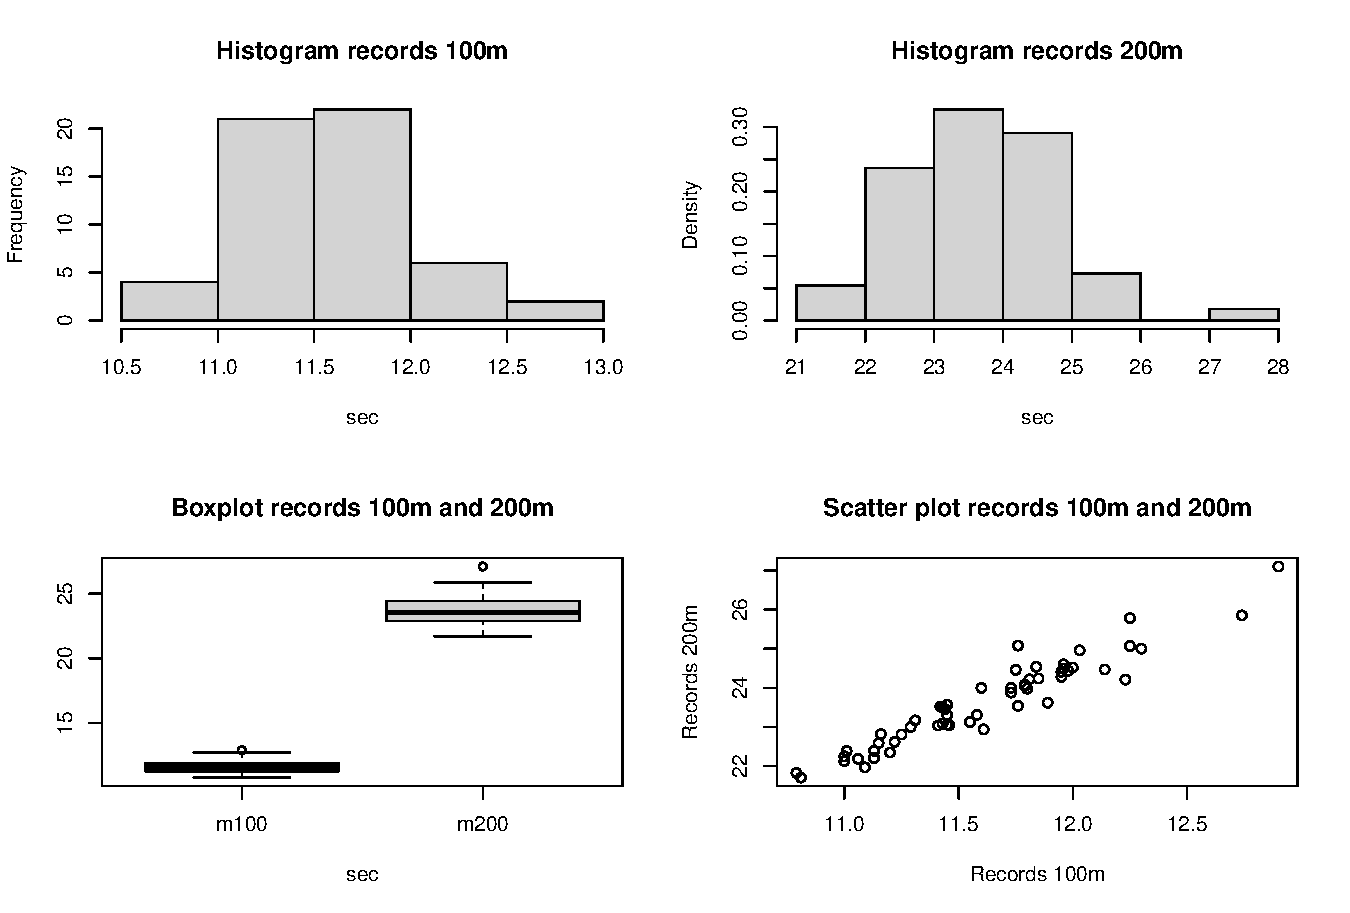
\includegraphics[width=\textwidth]{img/example-analysis-of-quantitative-data-3.pdf}
        \caption*{Using \texttt{par} command}
    \end{figure}

    \begin{figure}[!htp]
        \centering
        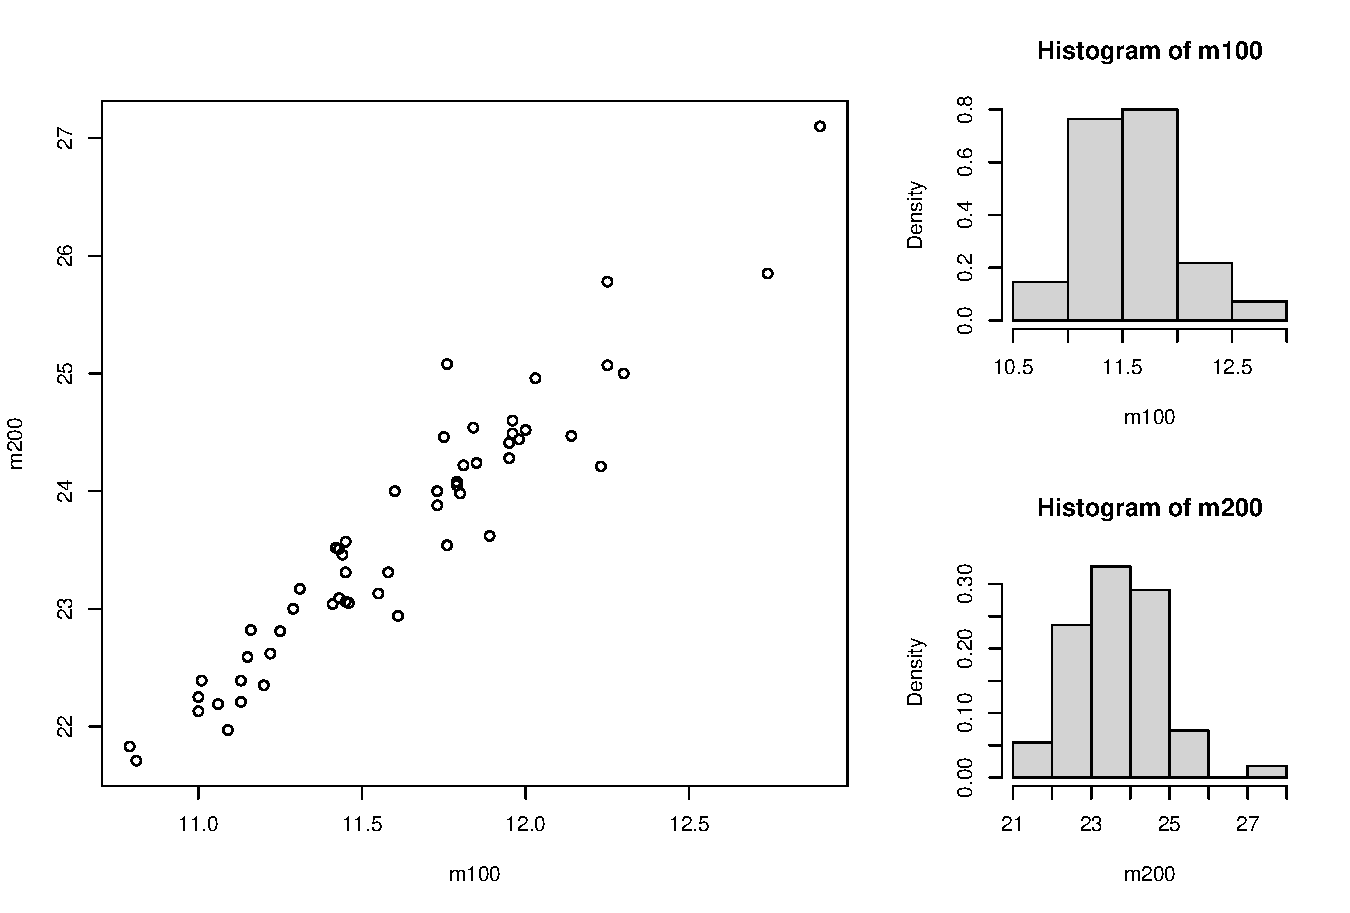
\includegraphics[width=\textwidth]{img/example-analysis-of-quantitative-data-4.pdf}
        \caption*{Using \texttt{layout} command}
    \end{figure}

    \newpage

    \noindent
    Now we calculate the regression using the function:
    \begin{itemize}
        \item \texttt{lm} is used \textbf{to fit linear models}, including multivariate ones. It can be used to carry out regression, single stratum analysis of variance and analysis of covariance. Arguments:
        \begin{itemize}
            \item \texttt{formula}: a symbolic description of the model to be fitted.
        \end{itemize}
    \end{itemize}
    Models for \texttt{lm} are specified symbolically. A typical model has the form \texttt{response} $\sim$ \texttt{terms} where 
    \begin{itemize}
        \item \texttt{response} is the (numeric) response vector.
        \item \texttt{terms} is a series of terms which specifies a linear predictor for response.
    \end{itemize}
    A terms specification of the form:
    \begin{itemize}
        \item \texttt{first + second} indicates all the terms in \texttt{first} together with all the terms in \texttt{second} with duplicates removed.
        
        \item \texttt{first:second} indicates the set of terms obtained by taking the interactions of all terms in \texttt{first} with all terms in \texttt{second}.

        \item \texttt{first*second} indicates the \emph{cross} of \texttt{first} and \texttt{second}. This is the same as \texttt{first + second + first:second}.
    \end{itemize}
    \underline{\textbf{Note 1}}: tilde $\sim$ is used to separate the left- and right-hand sides in a model formula.

    \noindent
    \underline{\textbf{Note 2}}: \texttt{summary} is a generic function used to produce result summaries of the results of various model fitting functions. The function invokes particular methods which depend on the class of the first argument.
    \lstinputlisting[language=R, firstline=19, lastline=47]{code/example-analysis-of-quantitative-data-2.r}

    \newpage

    With the regression it is possible to calculate some interesting values:
    \begin{itemize}
        \item \texttt{coef} is a generic function which \textbf{extracts model coefficients} from objects returned by modeling functions. \texttt{coefficients} is an alias for it.

        \item \texttt{vcov} returns the \textbf{variance-covariance} matrix of the main parameters of a fitted model object. The \dquotes{main} parameters of model correspond to those returned by \texttt{coef}, and typically do not contain a nuisance scale parameter (sigma).

        \item \texttt{residuals} is a generic function which \textbf{extracts model residuals} from objects returned by modeling functions.

        \item \texttt{fitted} is a generic function which \textbf{extracts fitted values} from objects returned by modeling functions. \texttt{fitted.values} is an alias for it.
    \end{itemize}
    In the following code we use:
    \begin{itemize}
        \item \texttt{abline} adds one or more straight lines through the current plot.

        \item \texttt{points} is a generic function to draw a sequence of points at the specified coordinates. The specified character(s) are plotted, centered at the coordinates.

        \item \texttt{legend} used to add legends to plots. Arguments:
        \begin{itemize}
            \item \texttt{x} (first argument), \texttt{y} (second argument): the x and y co-ordinates to be used to position the legend.

            \item \texttt{col}: the color of points or lines appearing in the legend.

            \item \texttt{lty}, \texttt{lwd}: the line types and widths for lines appearing in the legend. One of these two \emph{must} be specified for line drawing.

            \item \texttt{pch}: the plotting symbols appearing in the legend, as numeric vector or a vector of 1-character strings (see \texttt{points}). Unlike \texttt{points}, this can all be specified as a single multi-character string. \emph{Must} be specified for symbol drawing.
        \end{itemize}
    \end{itemize}
    \lstinputlisting[language=R, firstline=49, lastline=100]{code/example-analysis-of-quantitative-data-2.r}

    \newpage

    \begin{figure}[!htp]
        \centering
        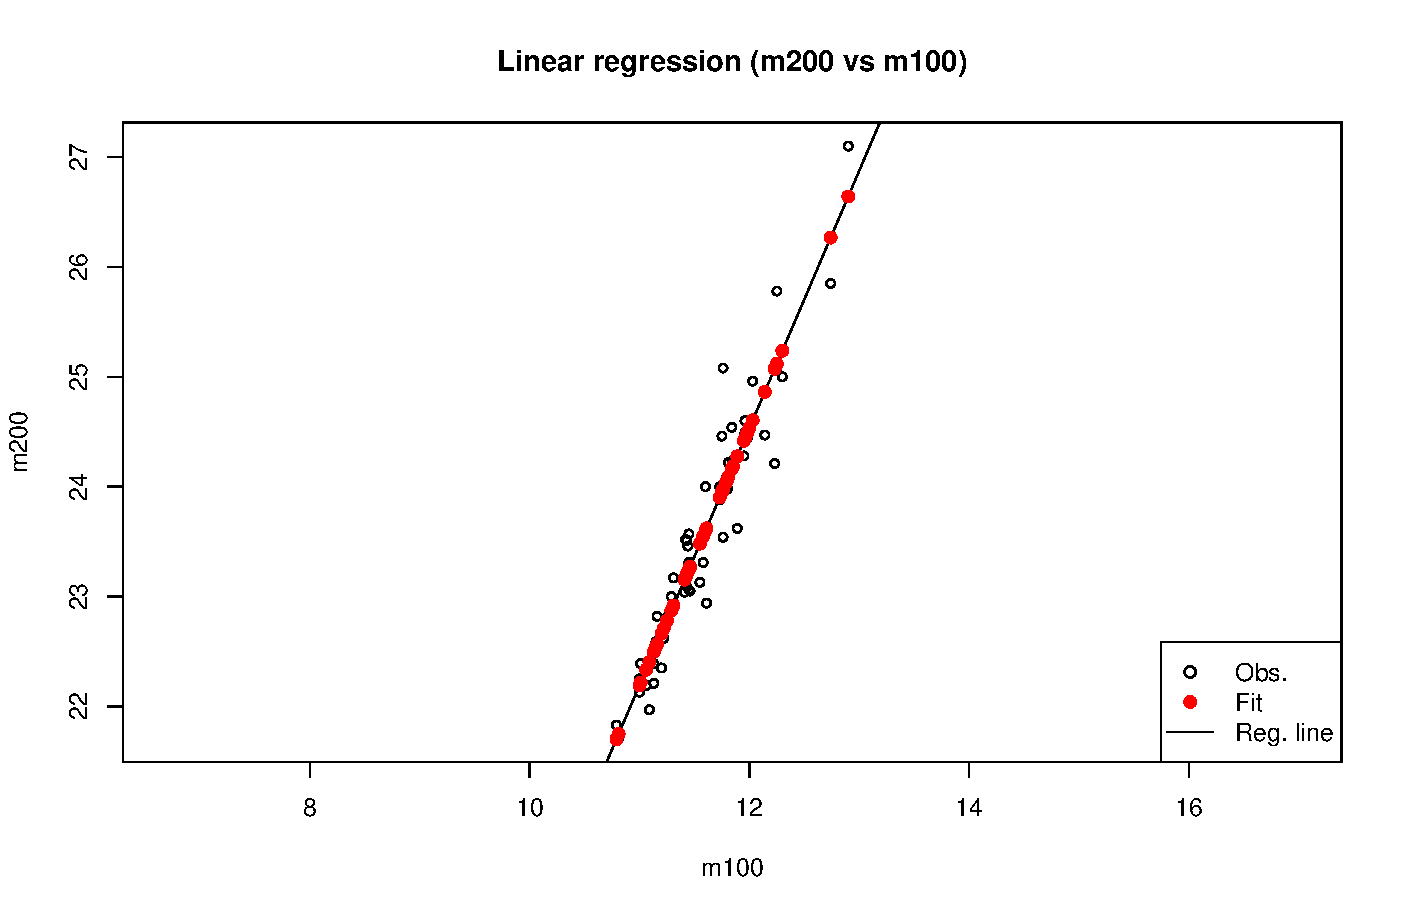
\includegraphics[width=\textwidth]{img/example-analysis-of-quantitative-data-5.pdf}
    \end{figure}

    \noindent
    We can do the F-test\footnote{An F-test is any statistical test used to compare the variances of two samples or the ratio of variances between multiple samples. The test statistic, random variable F, is used to determine if the tested data has an F-distribution under the true null hypothesis, and true customary assumptions about the error term ($\varepsilon$). It is most often used when comparing statistical models that have been fitted to a data set, in order to identify the model that best fits the population from which the data were sampled.} by hand:
    \lstinputlisting[language=R, firstline=102, lastline=111]{code/example-analysis-of-quantitative-data-2.r}
    Furthermore, we can calculate confidence and prediction interval using \texttt{predict} command:
    \begin{itemize}
        \item \texttt{predict} is a generic function for predictions from the results of various model fitting functions. The function invokes particular methods which depend on the class of the first argument.
    \end{itemize}

    \newpage

    \lstinputlisting[language=R, firstline=114, lastline=157]{code/example-analysis-of-quantitative-data-2.r}
    
    \newpage

    \begin{figure}[!htp]
        \centering
        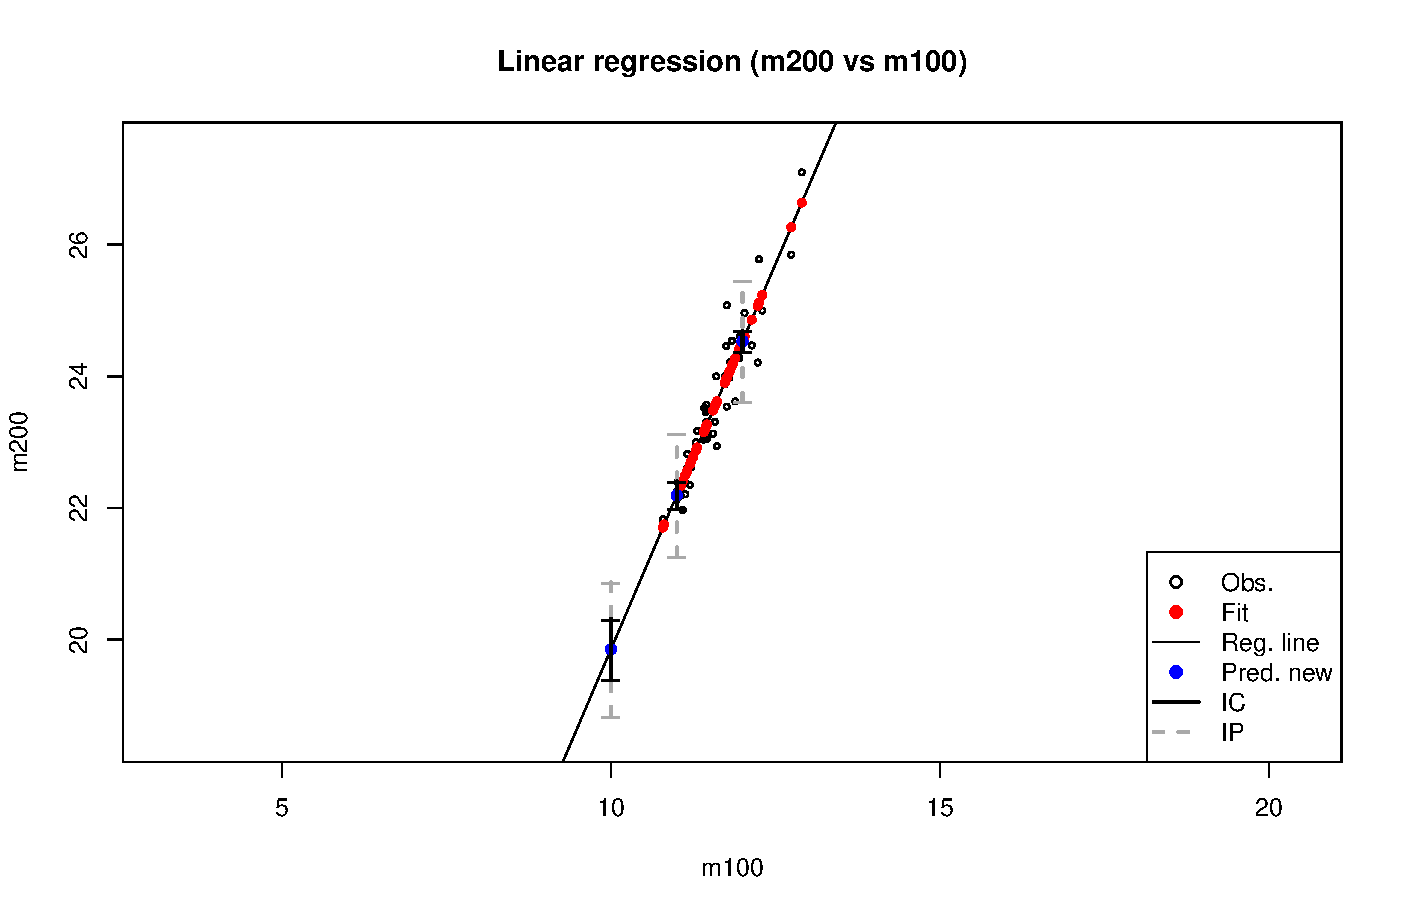
\includegraphics[width=\textwidth]{img/example-analysis-of-quantitative-data-6.pdf}
    \end{figure}

    \newpage

    \noindent
    Once we've fitted a regression model, it's a good idea to also produce \textbf{diagnostic plots} to analyze the residuals of the model and make sure that a linear model is appropriate for the particular data we're working with.

    \lstinputlisting[language=R, firstline=160, lastline=170]{code/example-analysis-of-quantitative-data-2.r}
    
    \begin{figure}[!htp]
        \centering
        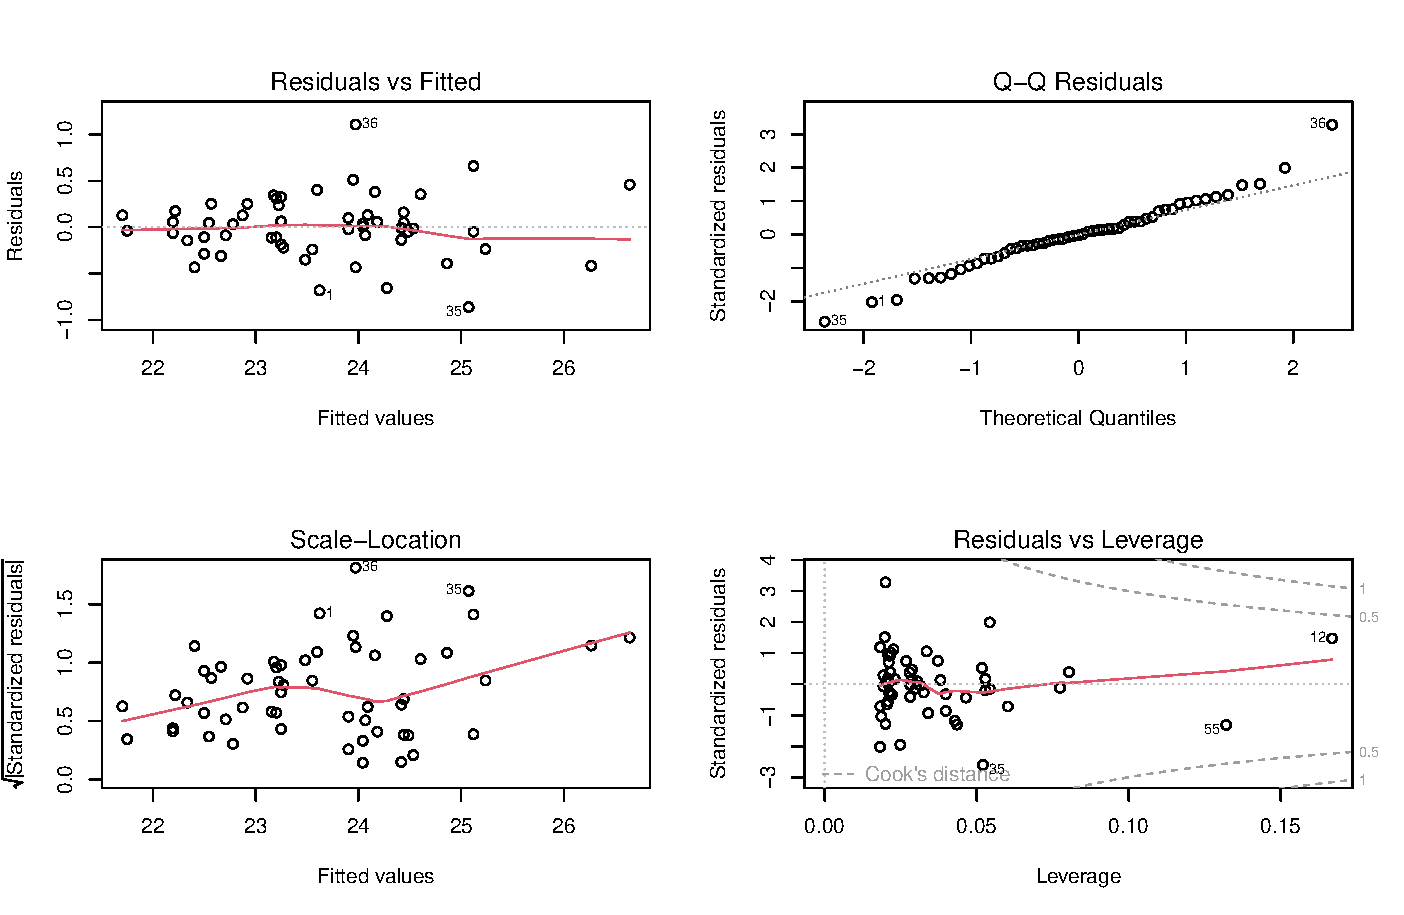
\includegraphics[width=\textwidth]{img/example-analysis-of-quantitative-data-7.pdf}
    \end{figure}

    \begin{itemize}
        \item \textcolor{Red3}{\texttt{Residuals vs Fitted}}. This plot is used to determine if the \textbf{residuals exhibit non-linear patterns}. If the red line across the center of the plot is roughly horizontal then we can assume that the residuals follow a linear pattern.
        
        In our example, we can see that the red line is almost the same as the perfect horizontal line. We declare that the residuals follow a roughly linear pattern and that a linear regression model is appropriate for this dataset.

        \item \textcolor{Red3}{\texttt{Q-Q residuals}}. This plot is used to determine if the \textbf{residuals of the regression model are normally distributed}. If the points in this plot fall roughly along a straight diagonal line, then we can assume the residuals are normally distributed.
        
        In our example, we can see that the points fall roughly along the straight diagonal line. We can then assume that the residuals are normally distributed.

        \newpage

        \item \textcolor{Red3}{\texttt{Scale-Location}}. This plot is used to \textbf{check the assumption of equal variance} (also called \href{https://en.wikipedia.org/wiki/Homoscedasticity_and_heteroscedasticity}{homoscedasticity}) \textbf{among the residuals in our regression model}. If the red line is roughly horizontal across the plot, then the assumption of equal variance is likely met.

        In our example, we can see that the red line isn't exactly horizontal across the plot, but it doesn't deviate too much at any point. We would probably say that the assumption of equal variance is not violated in this case.

        \item \textcolor{Red3}{\texttt{Residuals vs Leverage}}. This plot is used to \textbf{identify influential observations}. If any points in this plot fall outside of Cook's distance\footnote{In statistics, Cook's distance or Cook's D is a commonly used estimate of the influence of a data point when performing a least-squares regression analysis. In a practical ordinary least squares analysis, Cook's distance can be used in several ways: to indicate influential data points that are particularly worth checking for validity; or to indicate regions of the design space where it would be good to be able to obtain more data points.} (the dashed lines) then it is an influential observation.

        In our example we can see that observations 12, 35 and 55 are closest to the boundary of Cook's distance, but they don't fall outside the dashed line. This means that there aren't any overly influential points in our data set.
    \end{itemize}
    A useful guide to follow when creating diagnostic plots: \href{https://www.statology.org/diagnostic-plots-in-r/}{How to Interpret Diagnostic Plots in R}.

    \newpage

    \subsubsection{Visualization of multivariate data}

    \begin{flushleft}
        \example{Example 1: dataset record (all the variables)}
    \end{flushleft}
    Read the modified data created on page~\pageref{code: read.table - modded}:
    \lstinputlisting[language=R, firstline=1, lastline=9]{code/visualization-of-multivariate-data-1.r}
    Print the scatter plots of each column. We use the \texttt{pairs} function to automatically create a collage. But we could have used the \texttt{plot} function to get the same result.
    \lstinputlisting[language=R, firstline=11, lastline=12]{code/visualization-of-multivariate-data-1.r}
    \begin{figure}[!htp]
        \centering
        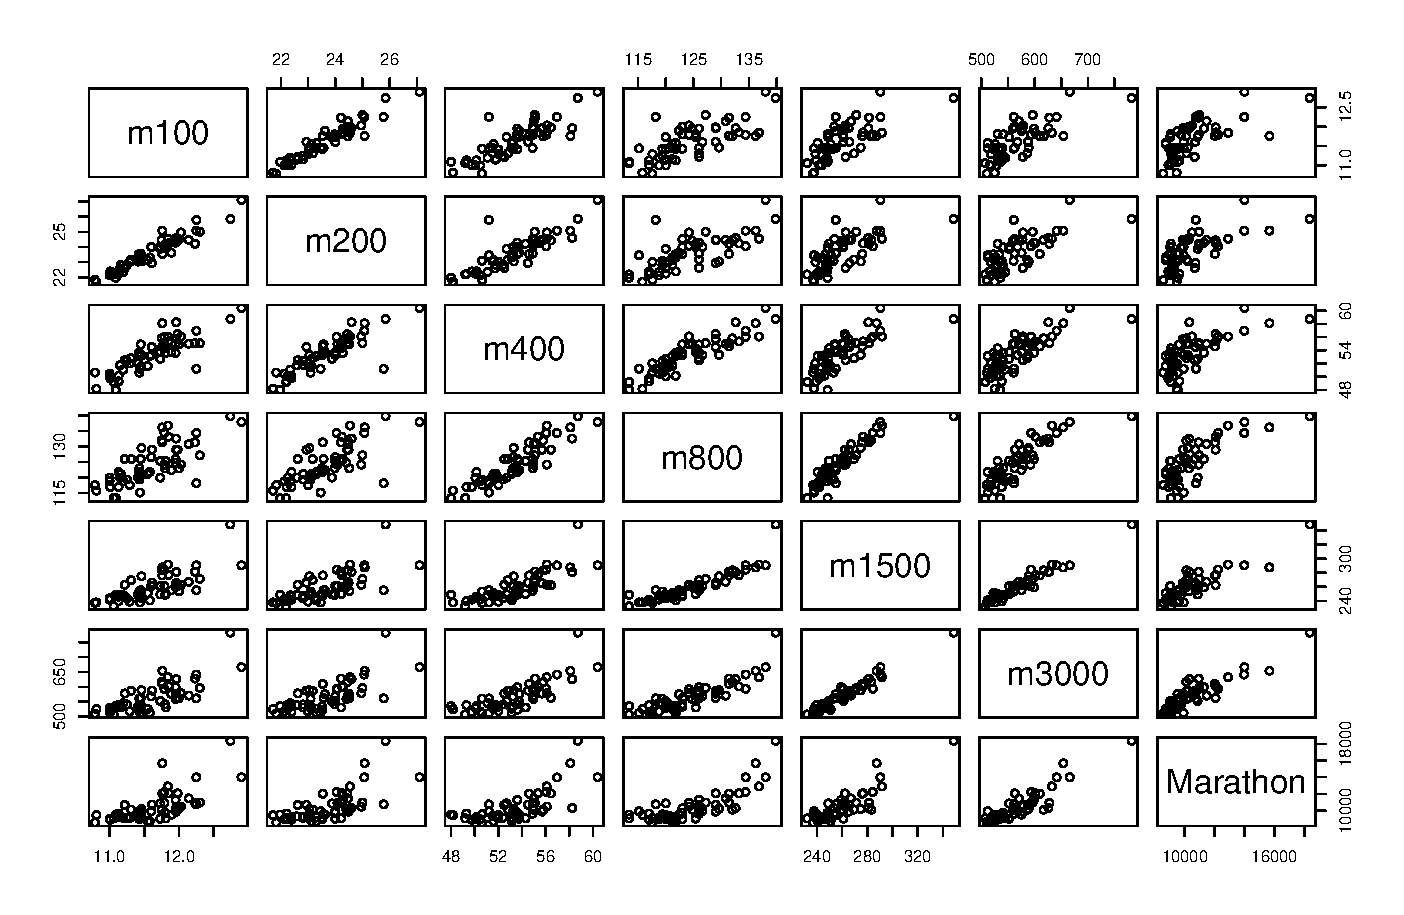
\includegraphics[width=\textwidth]{img/visualization-of-multivariate-data-1.pdf}
        \caption*{Image generated with the \texttt{pairs} function.}
    \end{figure}

    \newpage

    \noindent
    We print two box plots. The first is the data itself, the second is the logarithm. The second is more \dquotes{scaled} than the first.\footnote{See the following question: \href{https://stats.stackexchange.com/questions/211327/r-box-plot-on-log-scale-vs-log-transforming-then-creating-box-plot-dont-ge}{Cross Validated}}
    \lstinputlisting[language=R, firstline=14, lastline=17]{code/visualization-of-multivariate-data-1.r}
    \begin{figure}[!htp]
        \centering
        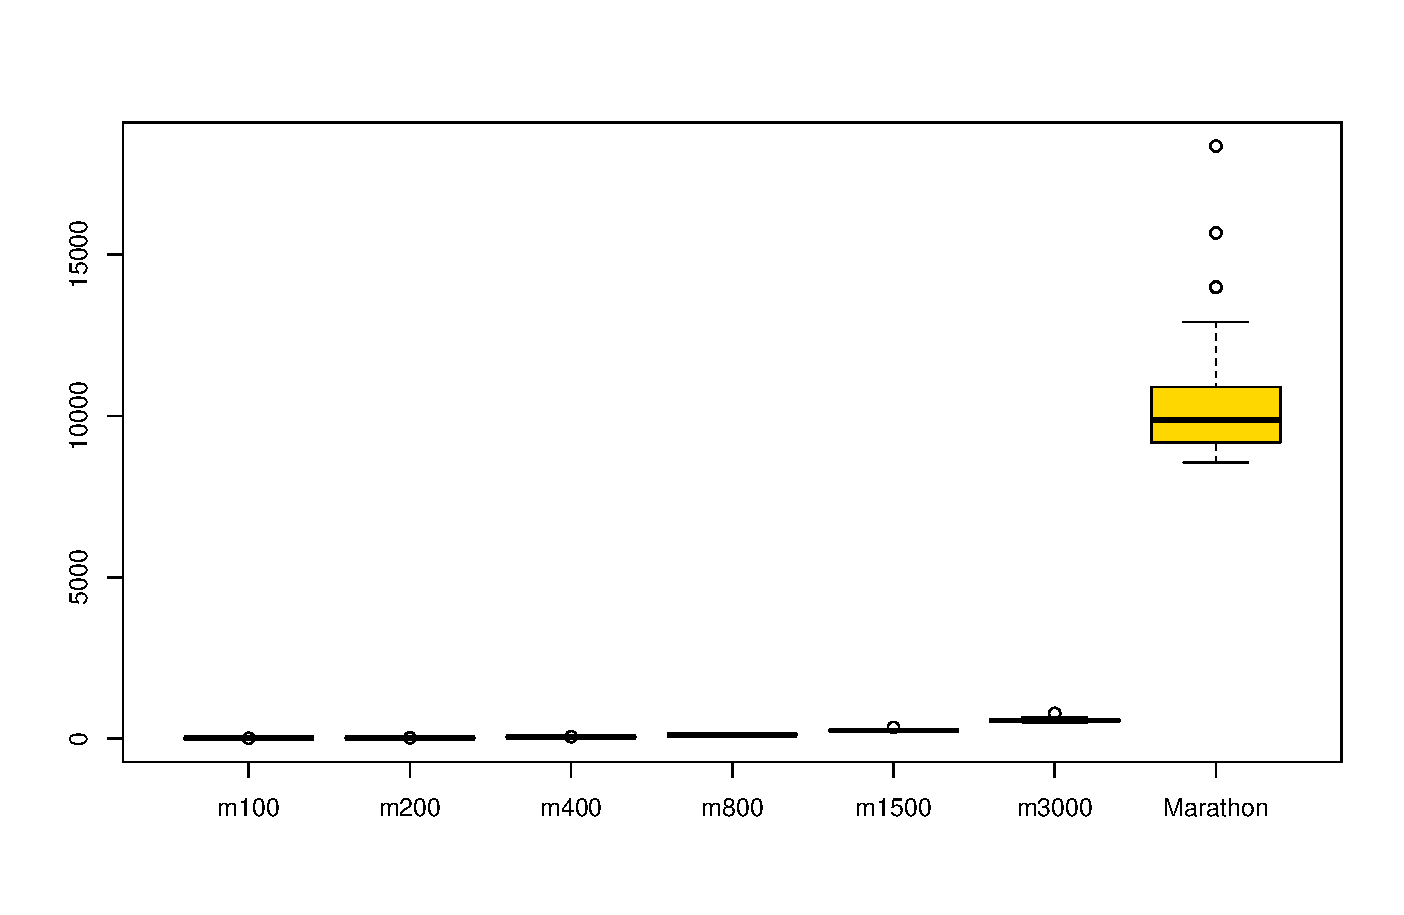
\includegraphics[width=\textwidth]{img/visualization-of-multivariate-data-2.pdf}
    \end{figure}
    \begin{figure}[!htp]
        \centering
        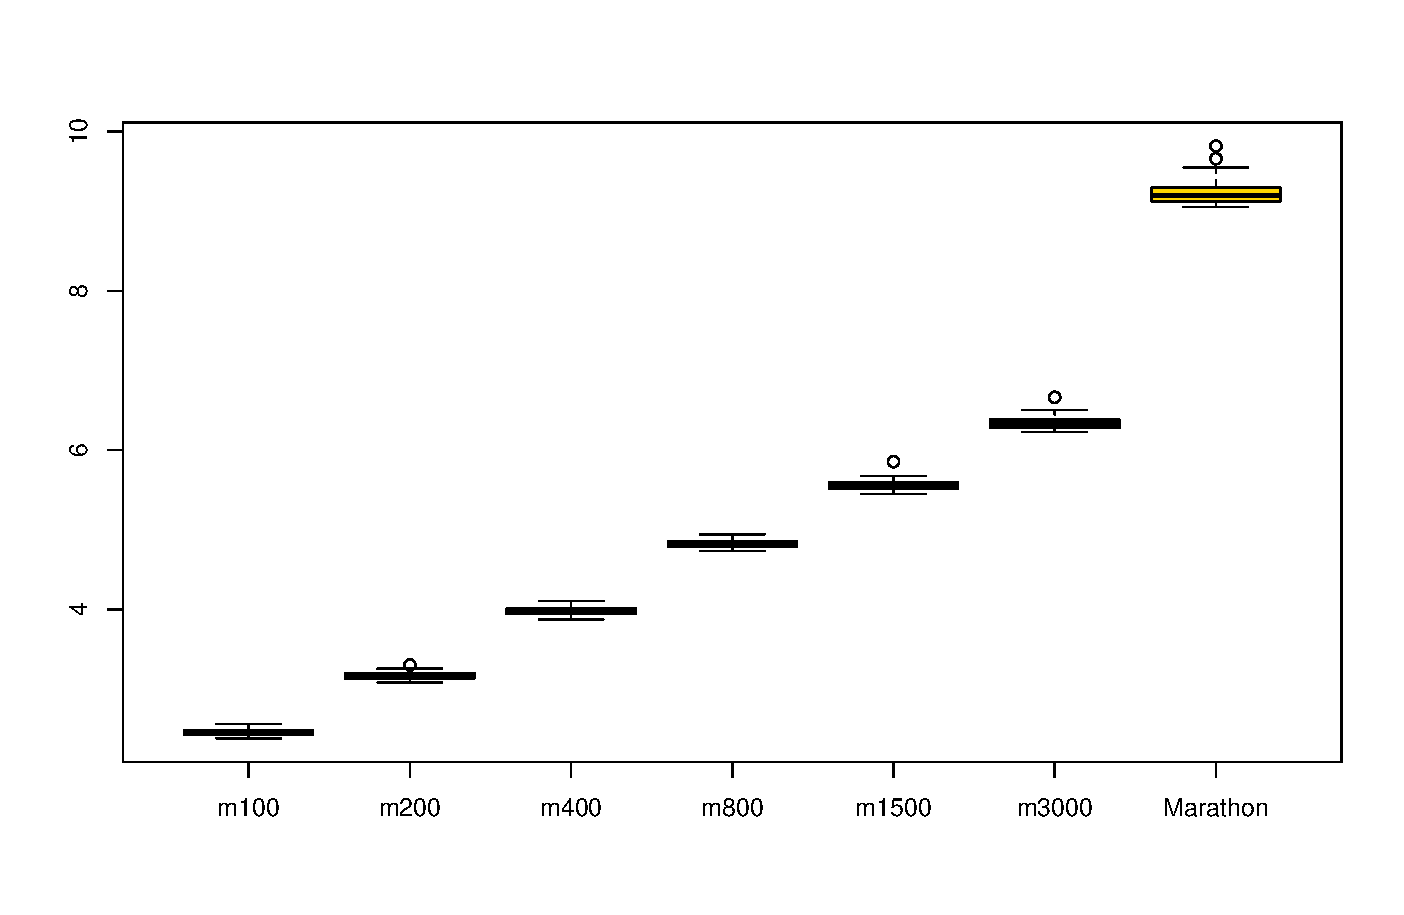
\includegraphics[width=\textwidth]{img/visualization-of-multivariate-data-3.pdf}
    \end{figure}

    \newpage

    \noindent
    Now, we use a star plot (or radar chart) for displaying multivariate data, in which each variable provides the measure of some common property of each observation. Each star in the plot represents a single observation. Star plot is used to examine the relative values of a single data point and locate similar and dissimilar points.

    \highspace
    The star plot consists of the sequence of equiangular spokes called radii with each spoke representing the value of observation on one of the variables. The data length of a spoke is proportional to the magnitude of the variable for the point related to the maximum data point in that variable. A line is drawn connecting to all the data points.\footnote{Source: \href{https://www.geeksforgeeks.org/star-charts-in-python/}{Star Charts in Python}}

    \highspace
    The star plot can be used to answer the following questions:
    \begin{itemize}
        \item which variable is dominant for a given observation?
        \item which observations are most similar i.e are there any clusters of observations?
        \item are there outliers?
    \end{itemize}
    The \texttt{stars} function draws star plots or segment diagrams of a multivariate data set.
    \begin{itemize}
        \item \texttt{col.stars}: color vector (integer or character), each specifying a color for one of the stars (cases). Ignored if \texttt{draw.segments = TRUE}.

        \item \texttt{draw.segments}: logical. If \texttt{TRUE} draw a segment diagram.
    \end{itemize}
    \lstinputlisting[language=R, firstline=19, lastline=23]{code/visualization-of-multivariate-data-1.r}
    \begin{figure}[!htp]
        \centering
        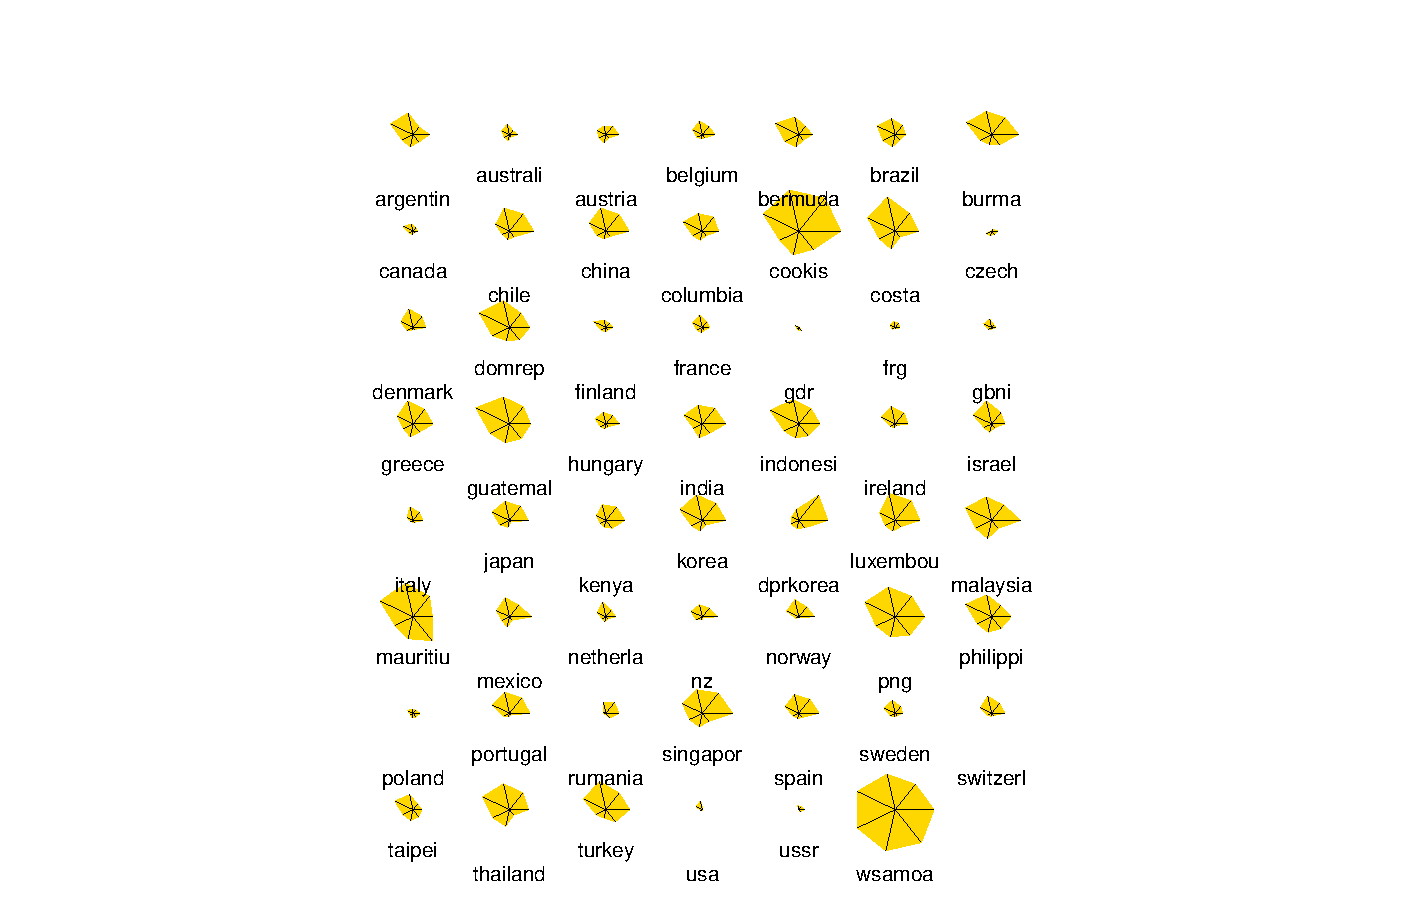
\includegraphics[width=\textwidth]{img/visualization-of-multivariate-data-4.pdf}
        \caption*{Star plot.}
    \end{figure}
    \begin{figure}[!htp]
        \centering
        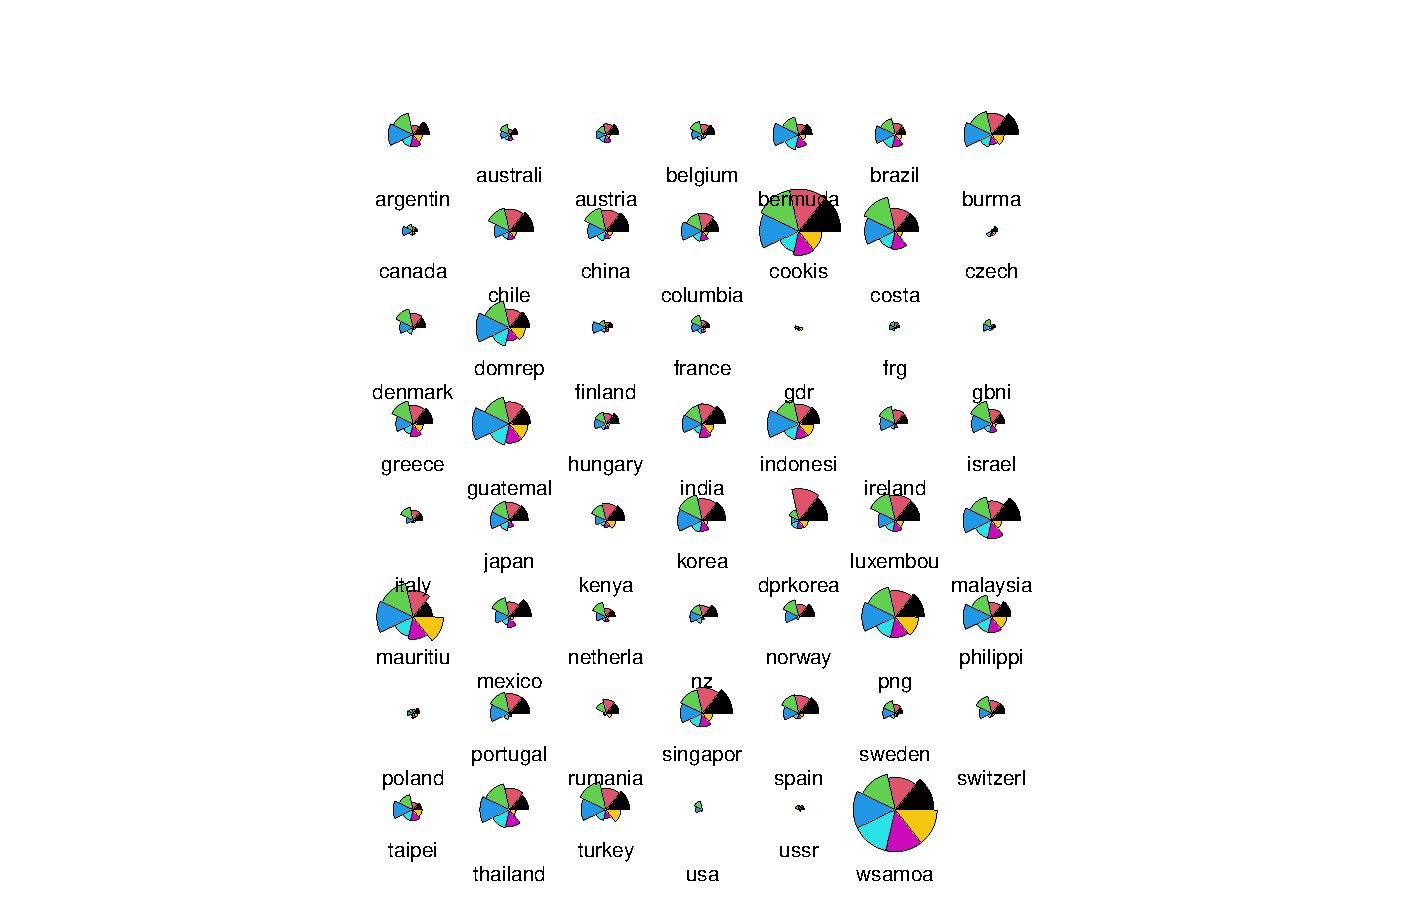
\includegraphics[width=\textwidth]{img/visualization-of-multivariate-data-5.pdf}
        \caption*{Radar plot.}
    \end{figure}

    \newpage

    \noindent
    Finally, we show the Chernoff faces. Invented by the applied mathematician, statistician and physicist Herman Chernoff in 1973, display multivariate data in the shape of a human face. The individual parts, such as eyes, ears, mouth and nose represent values of the variables by their shape, size, placement and orientation. 
    
    \highspace
    The idea behind using faces is that humans easily recognize faces and notice small changes without difficulty. Chernoff faces handle each variable differently. Because the features of the faces vary in perceived importance, the way in which variables are mapped to the features should be carefully chosen (e.g. eye size and eyebrow-slant have been found to carry significant weight).\cite{morris2000experimental}
    \lstinputlisting[language=R, firstline=25, lastline=27]{code/visualization-of-multivariate-data-1.r}
    \begin{figure}[!htp]
        \centering
        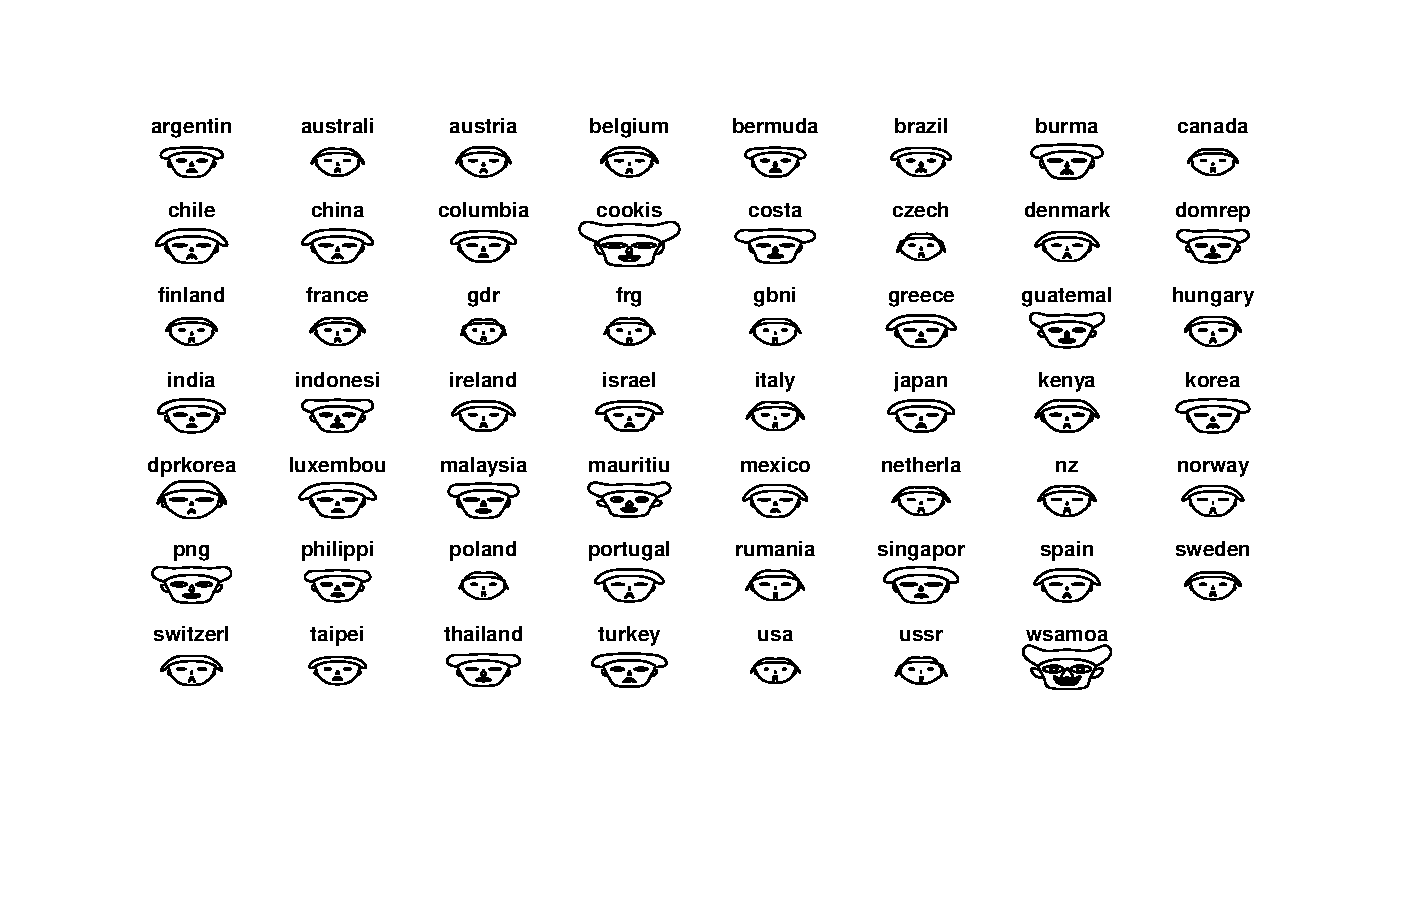
\includegraphics[width=\textwidth]{img/visualization-of-multivariate-data-6.pdf}
        \caption*{Chernoff faces.}
    \end{figure}

    \newpage

    \begin{flushleft}
        \example{Example 2: cerebral aneurysm}
    \end{flushleft}
    Given the following cerebral aneurysm data set:
    \lstinputlisting[language=R, firstline=1, lastline=71]{code/visualization-of-multivariate-data-2.r}
    We prepare the values. So we store the raw values in a \texttt{geometry} variable, and we store what \texttt{position} this data refers to. We also want to assign a red value if the position is 1, otherwise blue. So we use the \texttt{ifelse} function:
    \begin{itemize}
        \item \texttt{ifelse} returns a value with the same shape as \texttt{test} which is filled with elements selected from either \texttt{yes} or \texttt{no} depending on whether the element of \texttt{test} is \texttt{TRUE} or \texttt{FALSE}. Arguments:
        \begin{itemize}
            \item \texttt{test} an object which can be coerced to logical mode.
            \item \texttt{yes} return values for true elements of test.
            \item \texttt{no} return values for false elements of test.
        \end{itemize}
    \end{itemize}
    \lstinputlisting[language=R, firstline=74, lastline=93]{code/visualization-of-multivariate-data-2.r}
    Now we want to plot the data using the colors:
    \lstinputlisting[language=R, firstline=96, lastline=108]{code/visualization-of-multivariate-data-2.r}

    \newpage

    \begin{figure}[!htp]
        \centering
        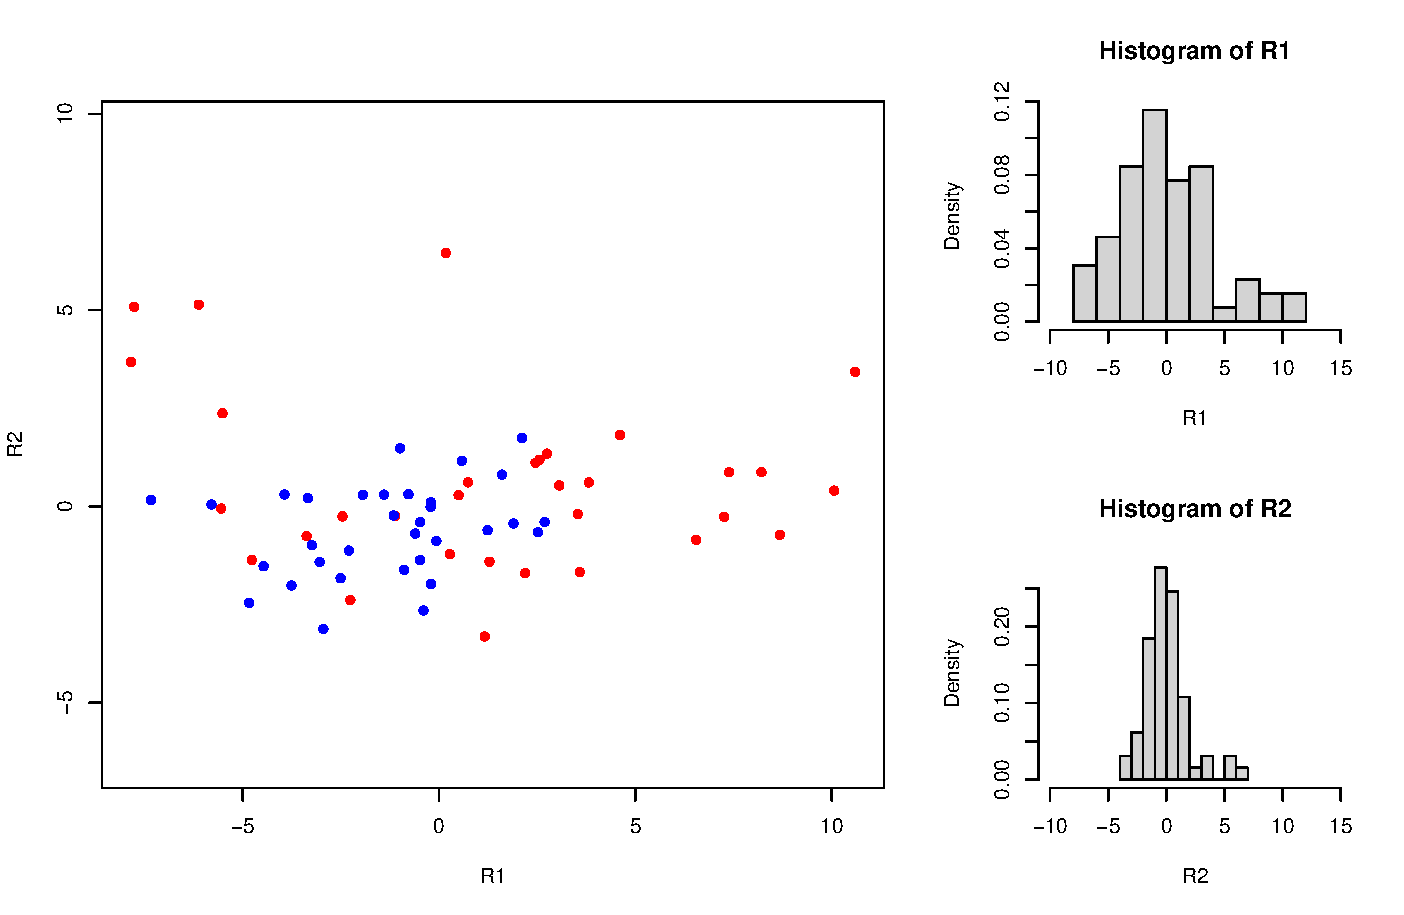
\includegraphics[width=\textwidth]{img/visualization-of-multivariate-data-7.pdf}
        \caption*{Compare R1 and R2.}
    \end{figure}

    \begin{figure}[!htp]
        \centering
        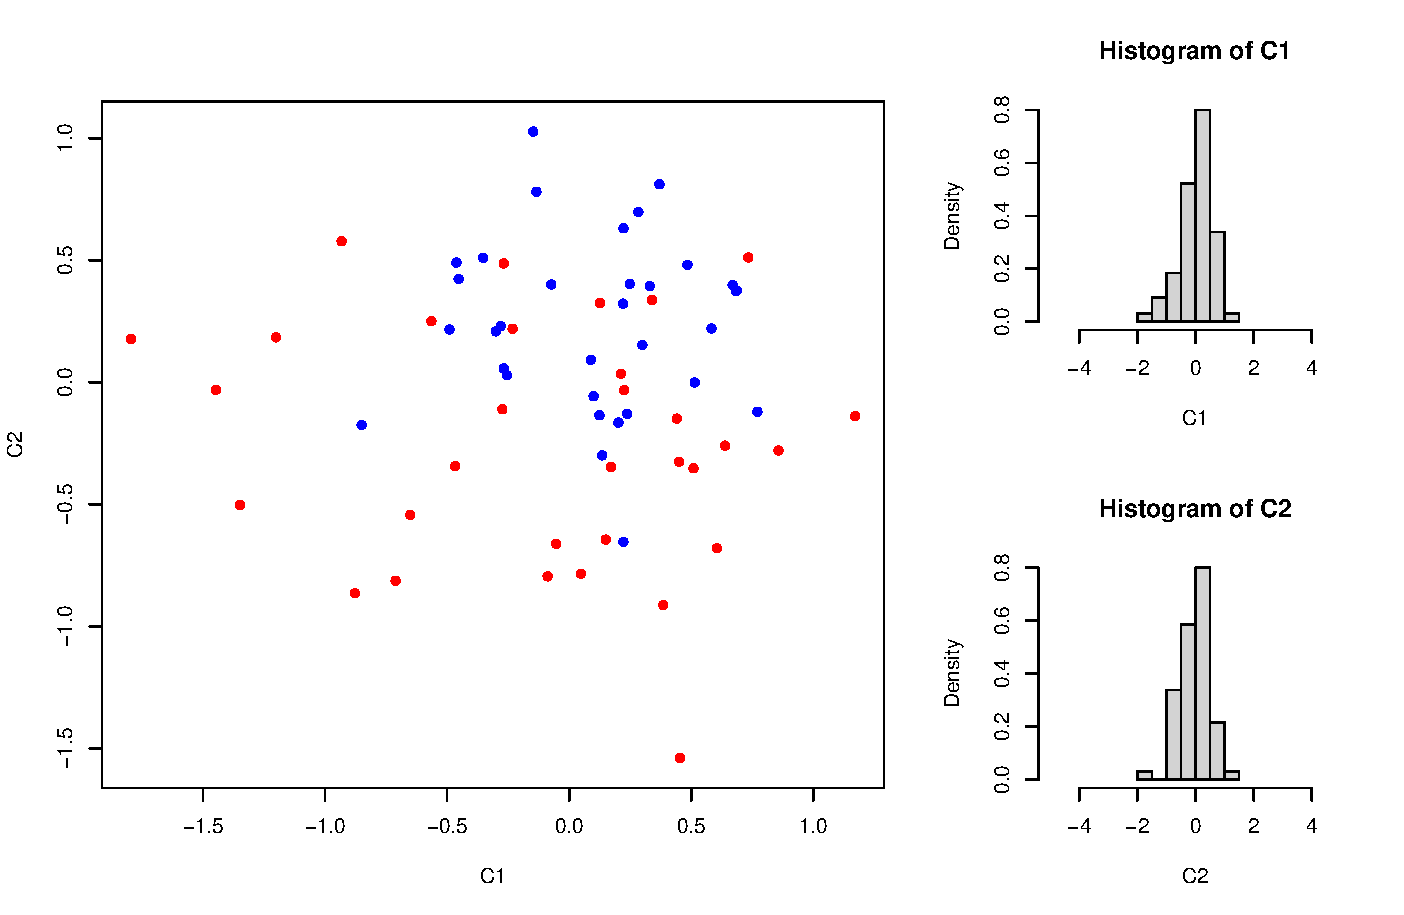
\includegraphics[width=\textwidth]{img/visualization-of-multivariate-data-8.pdf}
        \caption*{Compare C1 and C2.}
    \end{figure}

    \newpage

    \noindent
    We calculate the mean, the standard deviation, the covariance and the correlation. Using the \texttt{round} function, we get an approximation of the values. This can be useful to understand the data better. However, be careful when approximating numbers that are already less than 1.
    \begin{itemize}
        \item \texttt{round} function rounds the values in its first argument to the specified number of decimal places (default 0). Arguments:
        \begin{itemize}
            \item \texttt{x} a numeric/complex vector.
            \item \texttt{digits} integer indicating the number of decimal places.
        \end{itemize}
    \end{itemize}
    \lstinputlisting[language=R, firstline=111, lastline=151]{code/visualization-of-multivariate-data-2.r}

    \newpage

    \noindent
    It's always useful to create scatter plots to understand the location and variability of the points. We also print the box plot to see the distribution of the data, the outliers, etc. We have also used the same scale to understand if the median is approximately the same.
    \lstinputlisting[language=R, firstline=153, lastline=184]{code/visualization-of-multivariate-data-2.r}
    \begin{figure}[!htp]
        \centering
        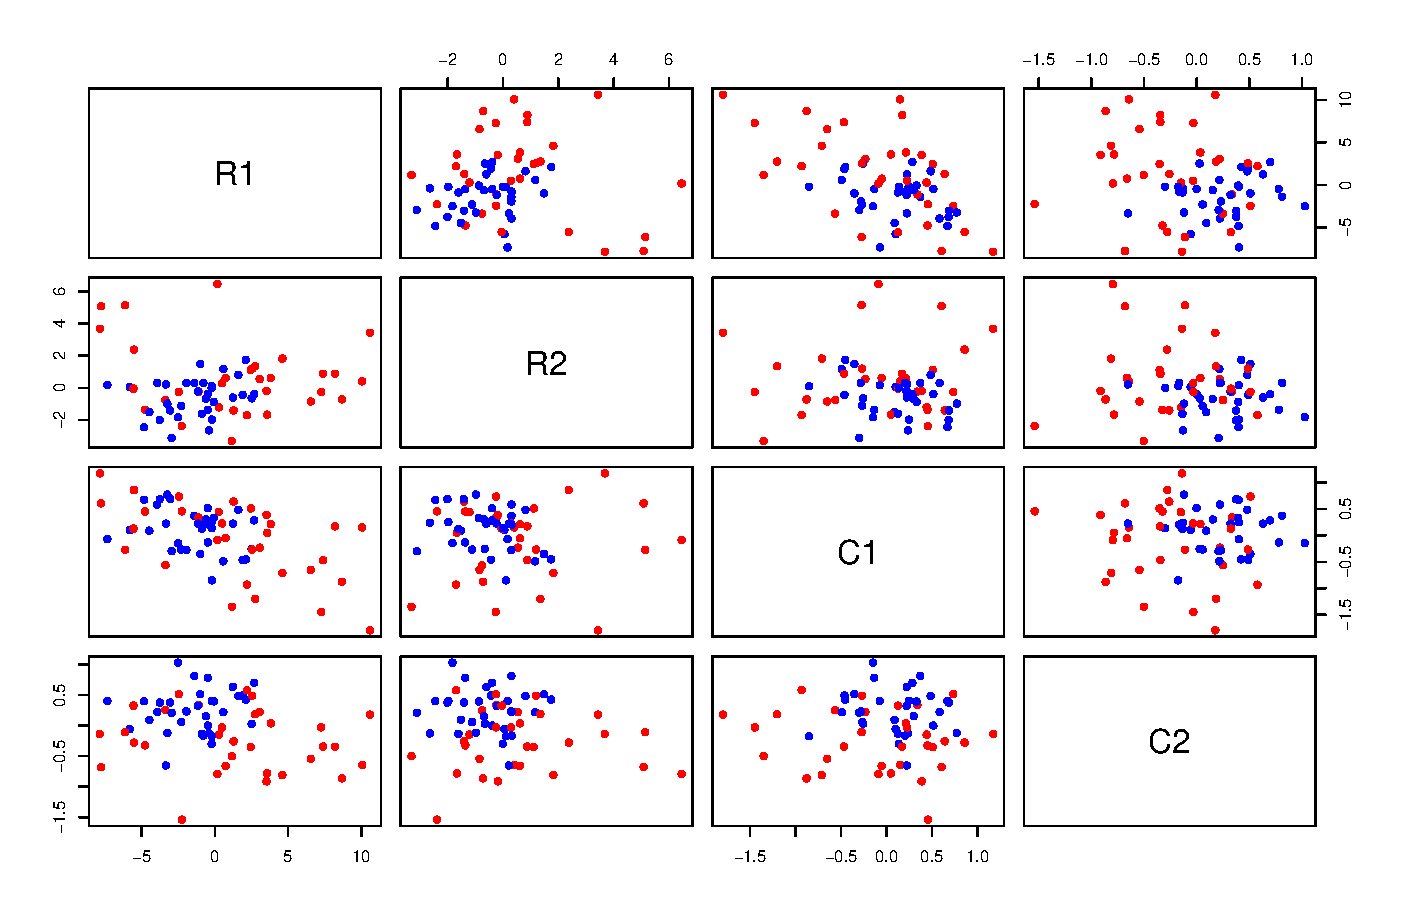
\includegraphics[width=\textwidth]{img/visualization-of-multivariate-data-9.pdf}
        \caption*{Scatter plot.}
    \end{figure}

    \begin{figure}[!htp]
        \centering
        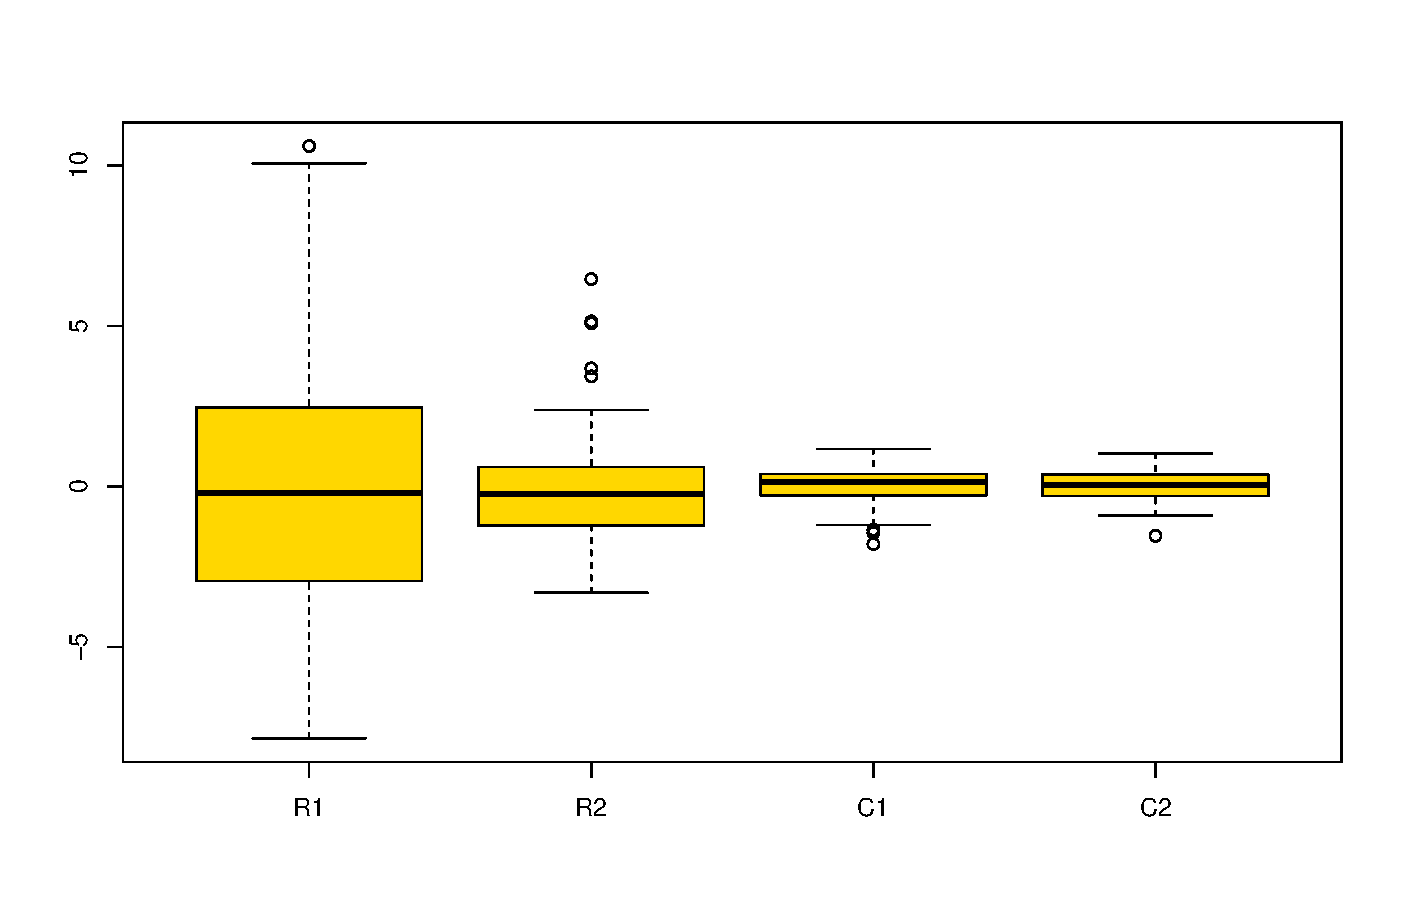
\includegraphics[width=\textwidth]{img/visualization-of-multivariate-data-10.pdf}
        \caption*{Box plot.}
    \end{figure}

    \begin{figure}[!htp]
        \centering
        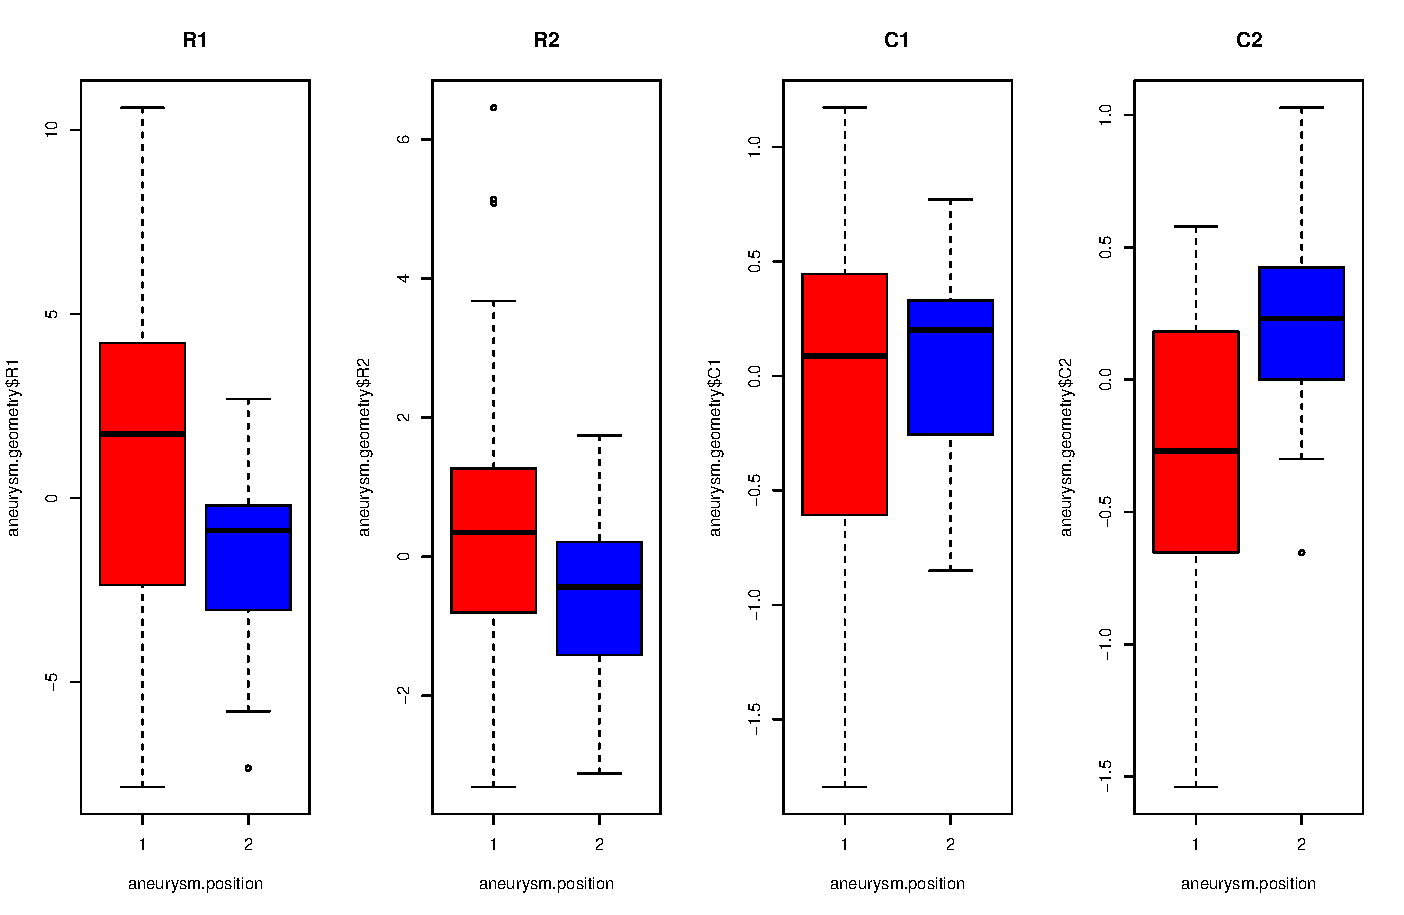
\includegraphics[width=\textwidth]{img/visualization-of-multivariate-data-11.pdf}
        \caption*{Stratified box plots.}
    \end{figure}

    \begin{figure}[!htp]
        \centering
        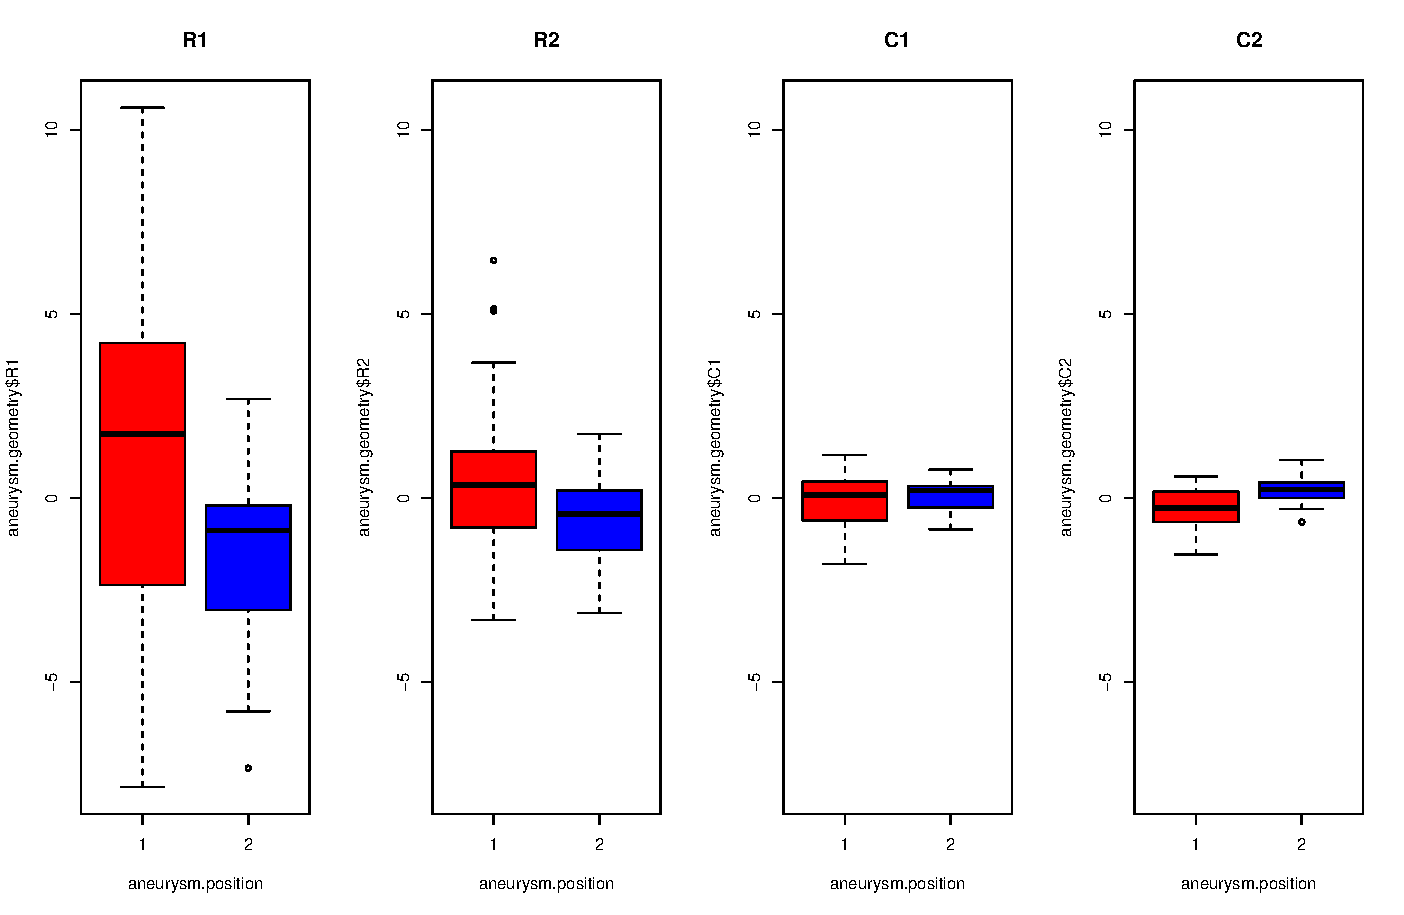
\includegraphics[width=\textwidth]{img/visualization-of-multivariate-data-12.pdf}
        \caption*{Stratified box plots (same scale).}
    \end{figure}

    \newpage

    \noindent
    Finally, we plot the Chernoff faces to easily detect small changes and we use the \texttt{matplot} function to plot the columns of the transposed \texttt{aneurysm.geometry} matrix.
    \lstinputlisting[language=R, firstline=187, lastline=194]{code/visualization-of-multivariate-data-2.r}
    \begin{figure}[!htp]
        \centering
        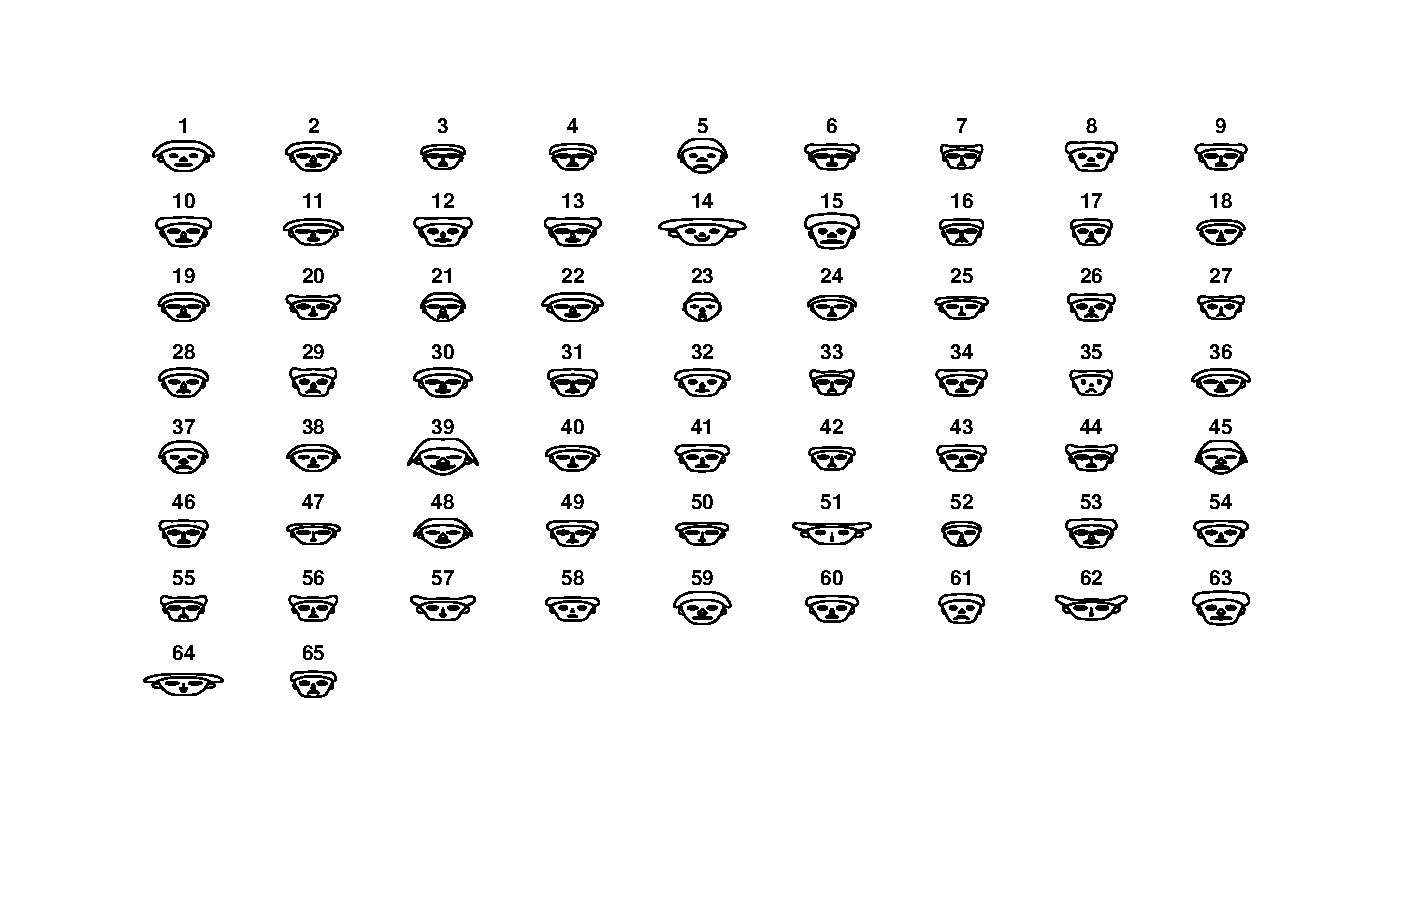
\includegraphics[width=\textwidth]{img/visualization-of-multivariate-data-13.pdf}
        \caption*{Chernoff faces.}
    \end{figure}

    \begin{figure}[!htp]
        \centering
        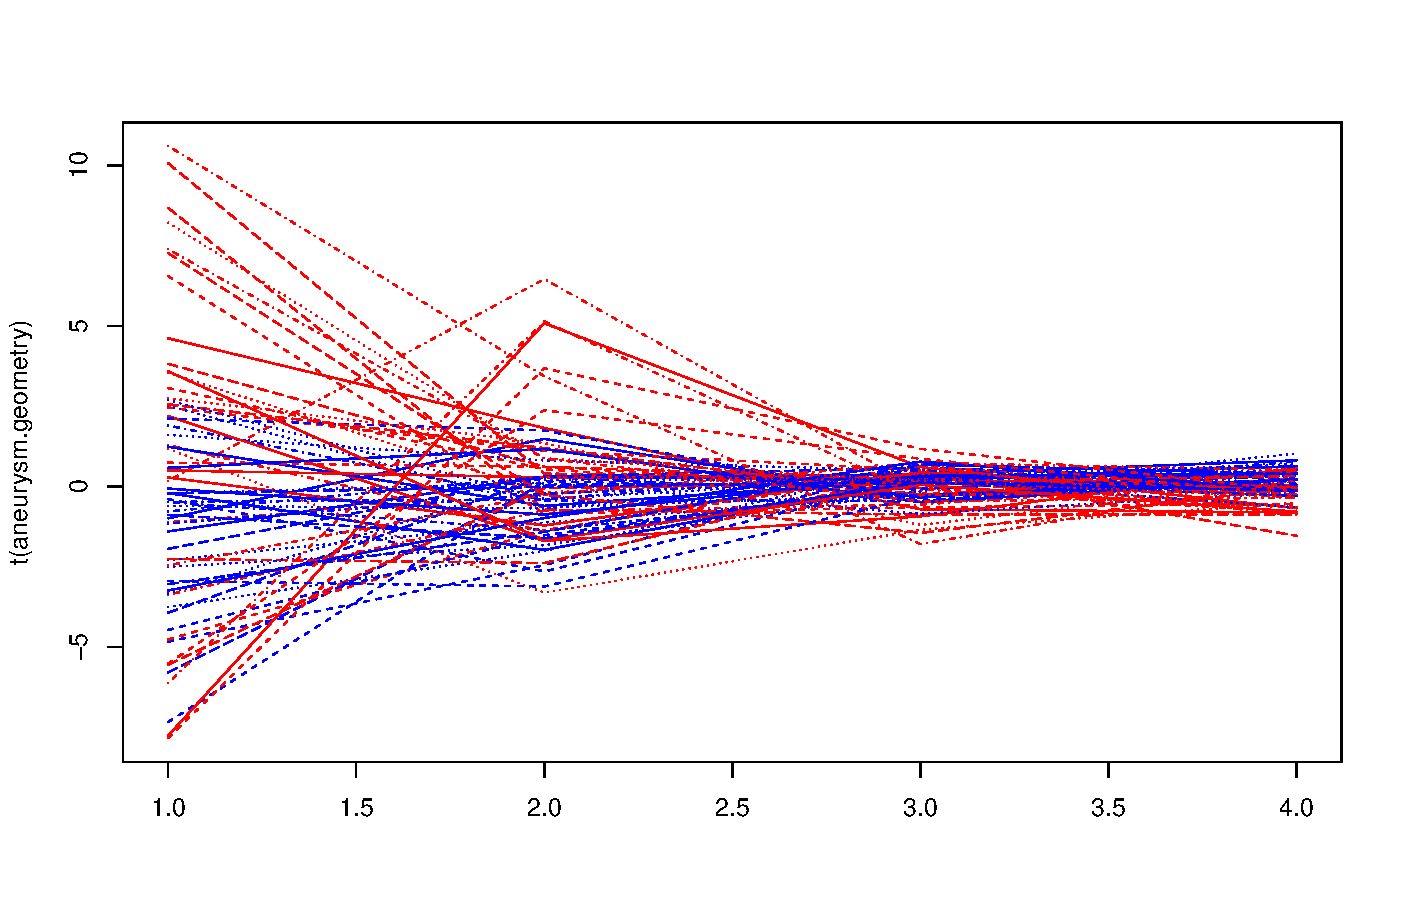
\includegraphics[width=\textwidth]{img/visualization-of-multivariate-data-14.pdf}
        \caption*{Result of the \texttt{matplot} function.}
    \end{figure}

    \newpage

    \subsubsection{Visualization of Categorical Data}

    It may be useful to plot a pie chart to see the categorical data. We then use the \texttt{pie} function, which draws a pie chart.
    \lstinputlisting[language=R, firstline=1, lastline=9]{code/visualization-of-categorical-data-1.r}
    \begin{figure}[!htp]
        \centering
        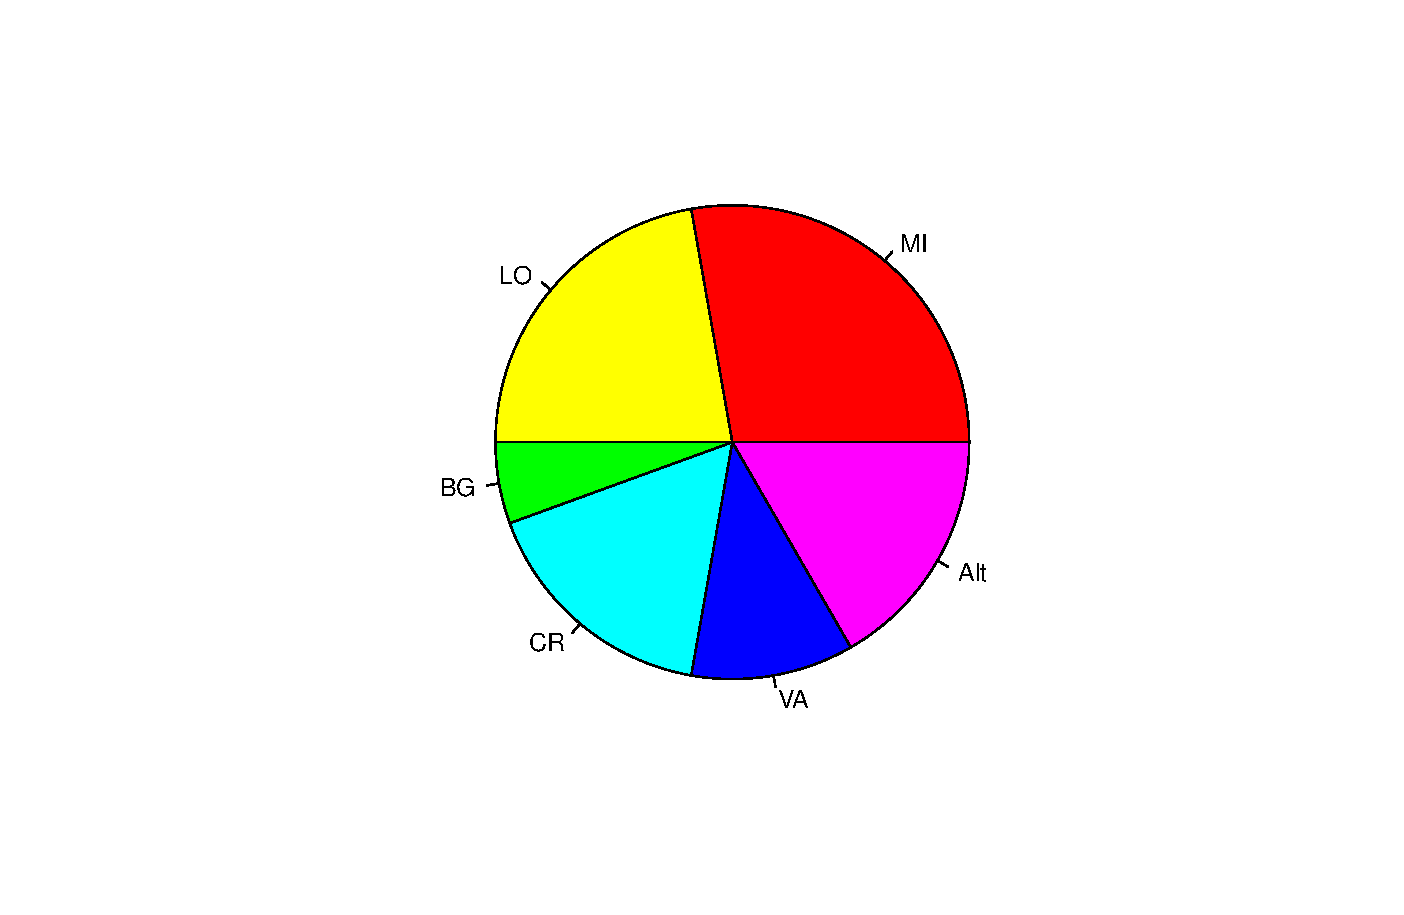
\includegraphics[width=.5\textwidth]{img/visualization-of-categorical-data-1.pdf}
        \caption*{Pie chart.}
    \end{figure}

    \noindent
    Also pay attention between the data inserted as argument in the \texttt{plot} function, because the behavior would be different (it depends on the object as input parameter).
    \lstinputlisting[language=R, firstline=12, lastline=28]{code/visualization-of-categorical-data-1.r}

    \newpage

    \begin{figure}[!htp]
        \centering
        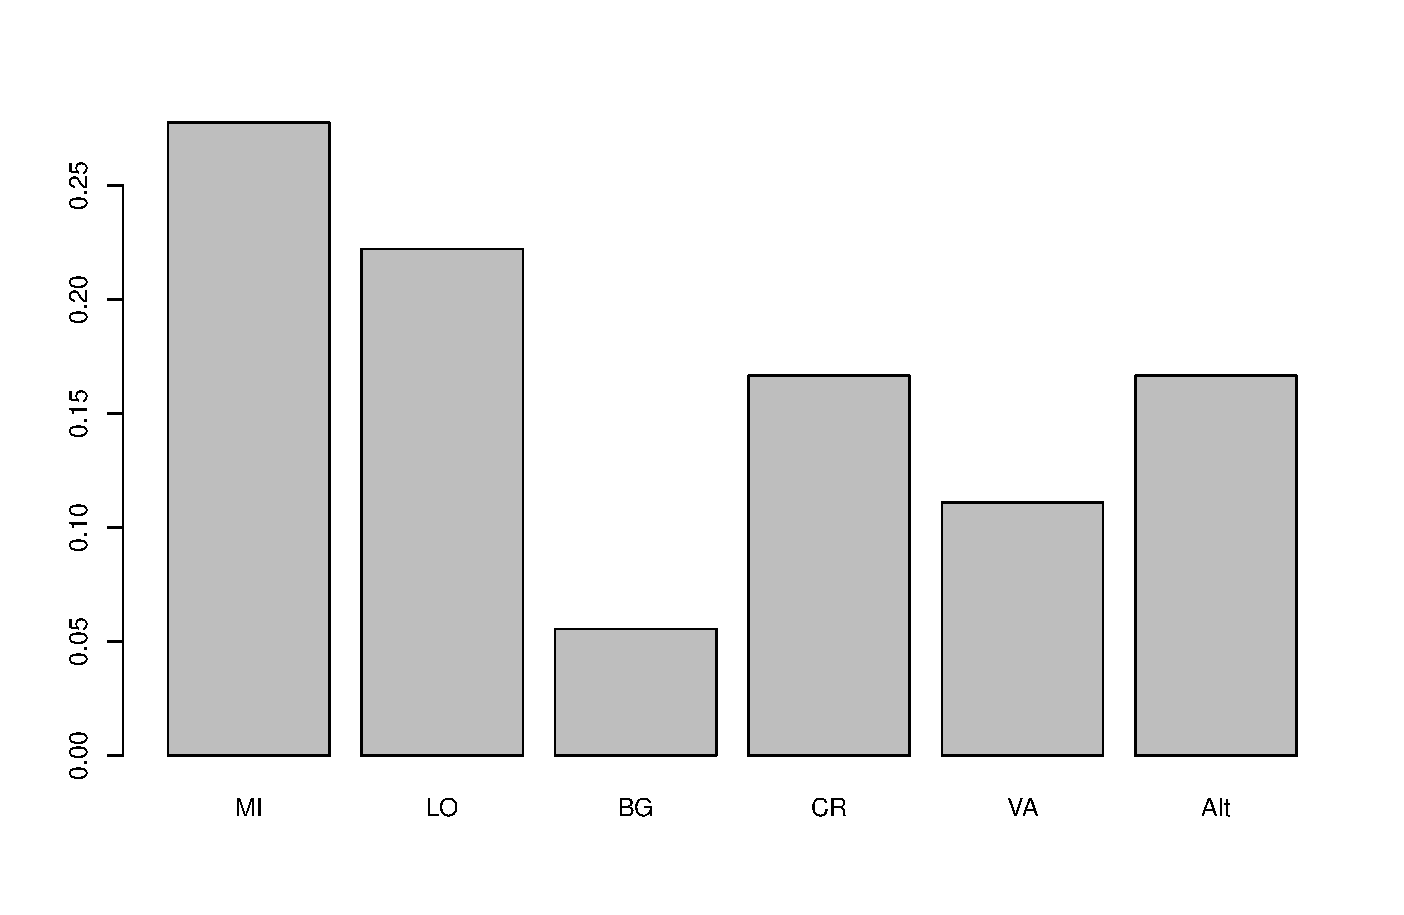
\includegraphics[width=\textwidth]{img/visualization-of-categorical-data-2.pdf}
        \caption*{Bar plot (levels are ordered).}
    \end{figure}

    \begin{figure}[!htp]
        \centering
        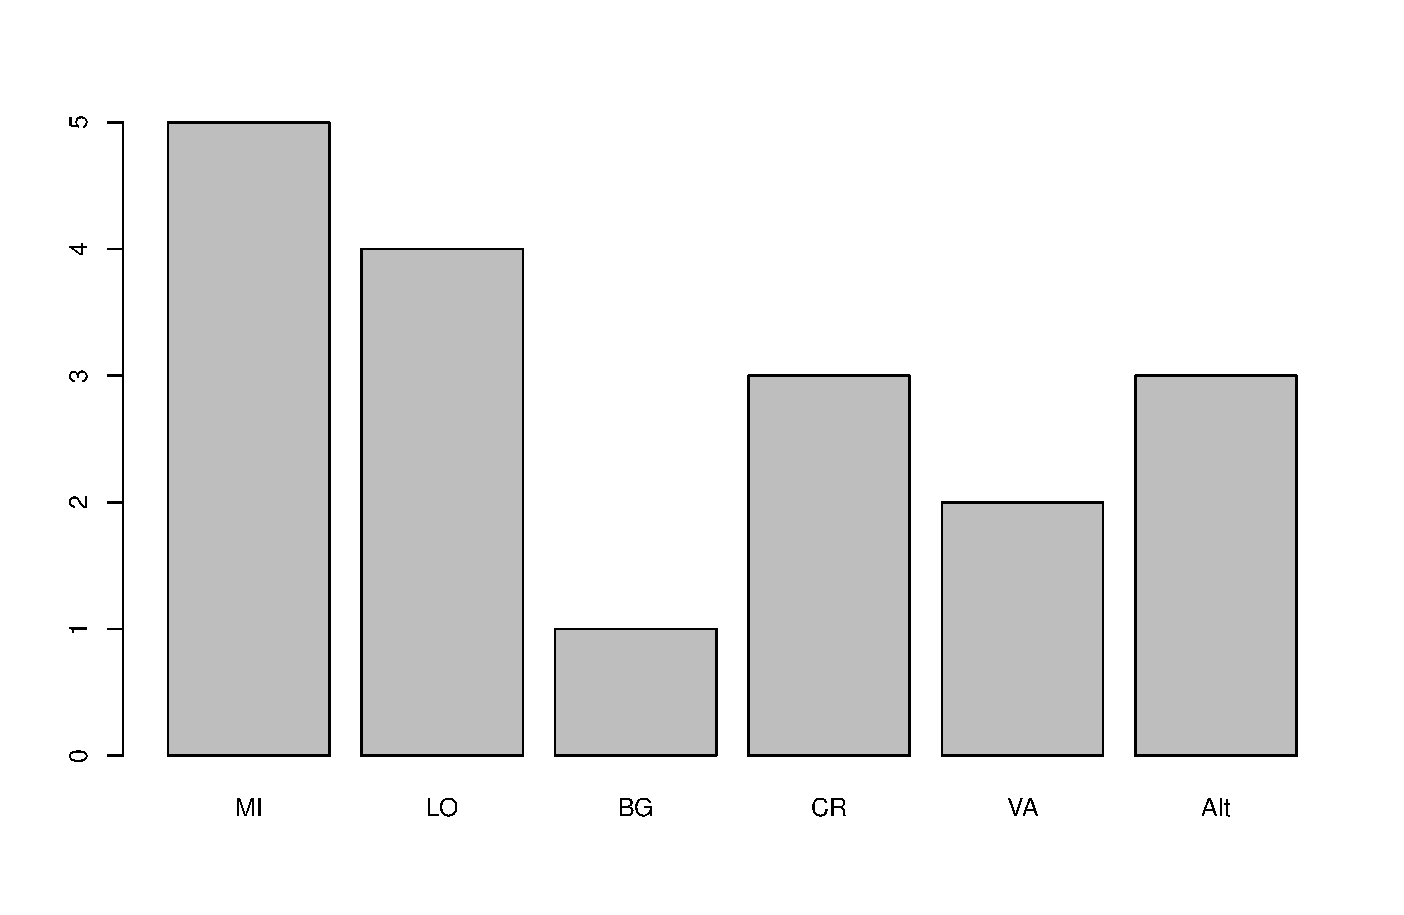
\includegraphics[width=\textwidth]{img/visualization-of-categorical-data-3.pdf}
        \caption*{Bar plot of absolute frequencies (\texttt{factor} object).}
    \end{figure}

    \newpage

    \begin{figure}[!htp]
        \centering
        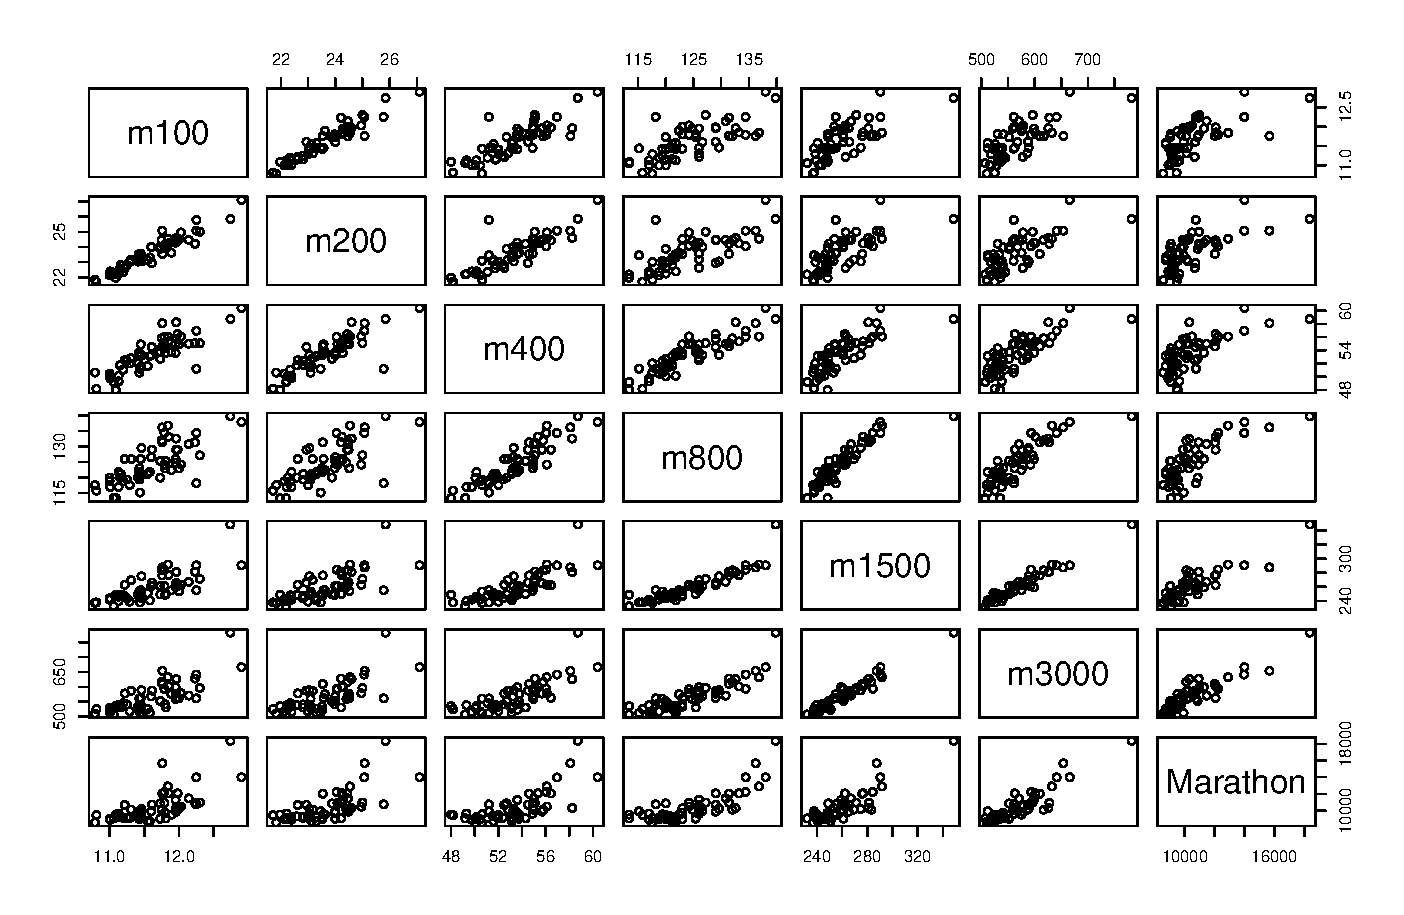
\includegraphics[width=\textwidth]{img/visualization-of-categorical-data-4.pdf}
        \caption*{Plot of the \texttt{data.frame} object.}
    \end{figure}

    \noindent
    Finally, be careful to the scale of representation.
    \lstinputlisting[language=R, firstline=31, lastline=35]{code/visualization-of-categorical-data-1.r}

    \begin{figure}[!htp]
        \centering
        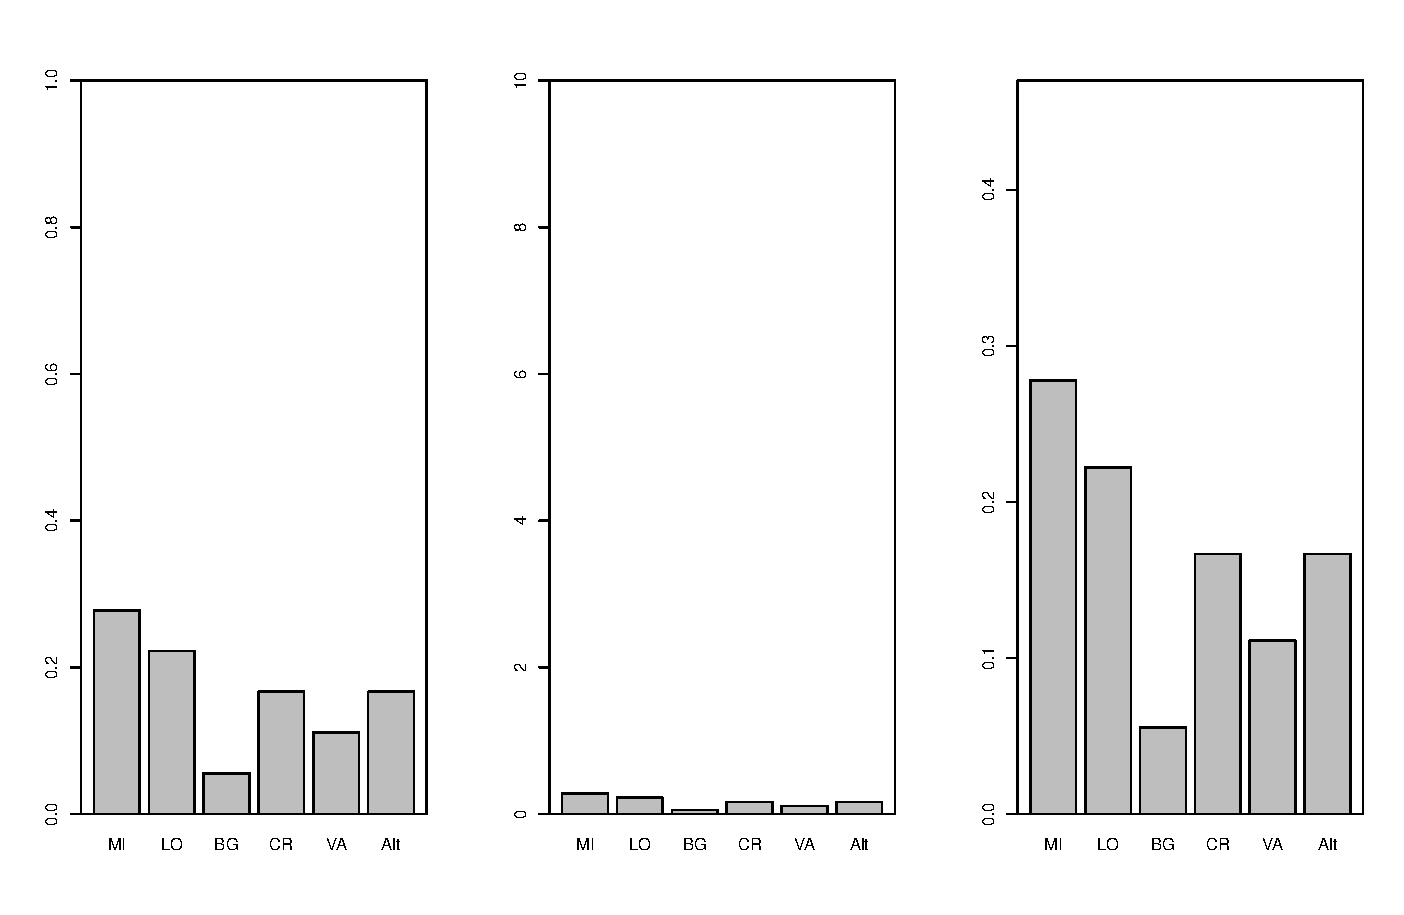
\includegraphics[width=\textwidth]{img/visualization-of-categorical-data-5.pdf}
        \caption*{Different scales of the same data.}
    \end{figure}

    \newpage

    \subsubsection{3D plots, functions, for loop and install new libraries}

    To create a function in \texttt{R}, the syntax is as follows:
    \lstinputlisting[language=R, firstline=1, lastline=8]{code/3d-plots-func-for-new-libs-1.r}
    A \texttt{for} loop can be created using the \texttt{for} keyword or the \texttt{outer} function.
    \begin{itemize}
        \item The \texttt{outer} product of the arrays \texttt{X} and \texttt{Y} is the array \texttt{A} with dimension \texttt{c(dim(X), dim(Y))} where element:
        \begin{center}
            \texttt{A[c(arrayindex.x, arrayindex.y)] = FUN(X[arrayindex.x], Y[arrayindex.y], ...)}
        \end{center}
        The arguments:
        \begin{itemize}
            \item \texttt{X}, \texttt{Y}: First and second arguments for function \texttt{FUN}. Typically a vector or array.
            
            \item \texttt{FUN}: a function to use on the outer products.
        \end{itemize}
    \end{itemize}
    \lstinputlisting[language=R, firstline=11, lastline=21]{code/3d-plots-func-for-new-libs-1.r}
    It's possible to create a grid of coloured or grey scale rectangles whose colors correspond to the values in the input argument (\texttt{image} function).
    \lstinputlisting[language=R, firstline=24, lastline=27]{code/3d-plots-func-for-new-libs-1.r}

    \newpage

    \begin{figure}[!htp]
        \centering
        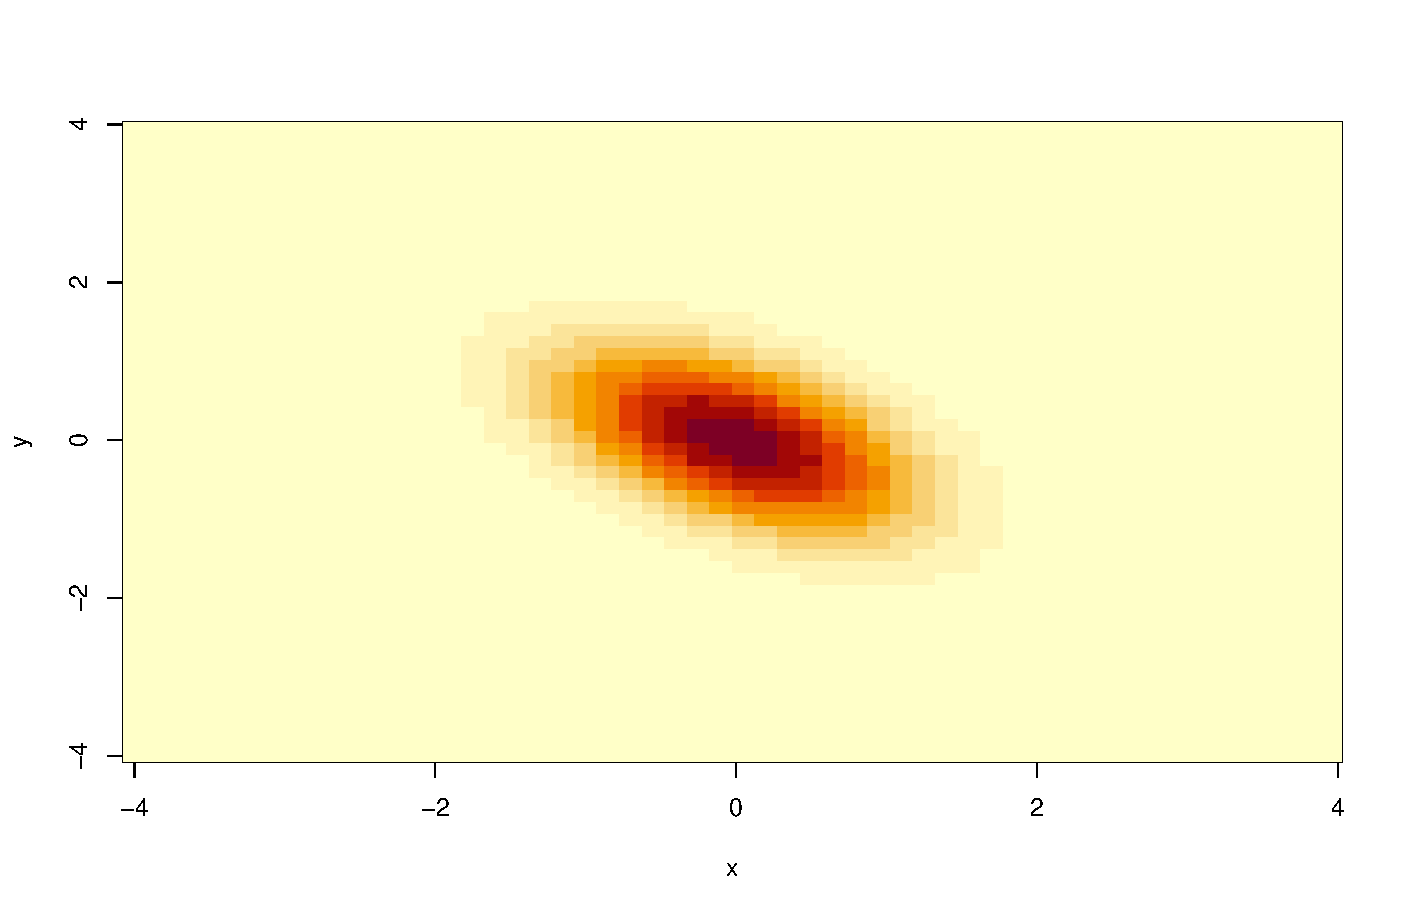
\includegraphics[width=\textwidth]{img/3d-plots-func-for-new-libs-1.pdf}
        \caption*{Image created with \texttt{image} function.}
    \end{figure}

    \begin{figure}[!htp]
        \centering
        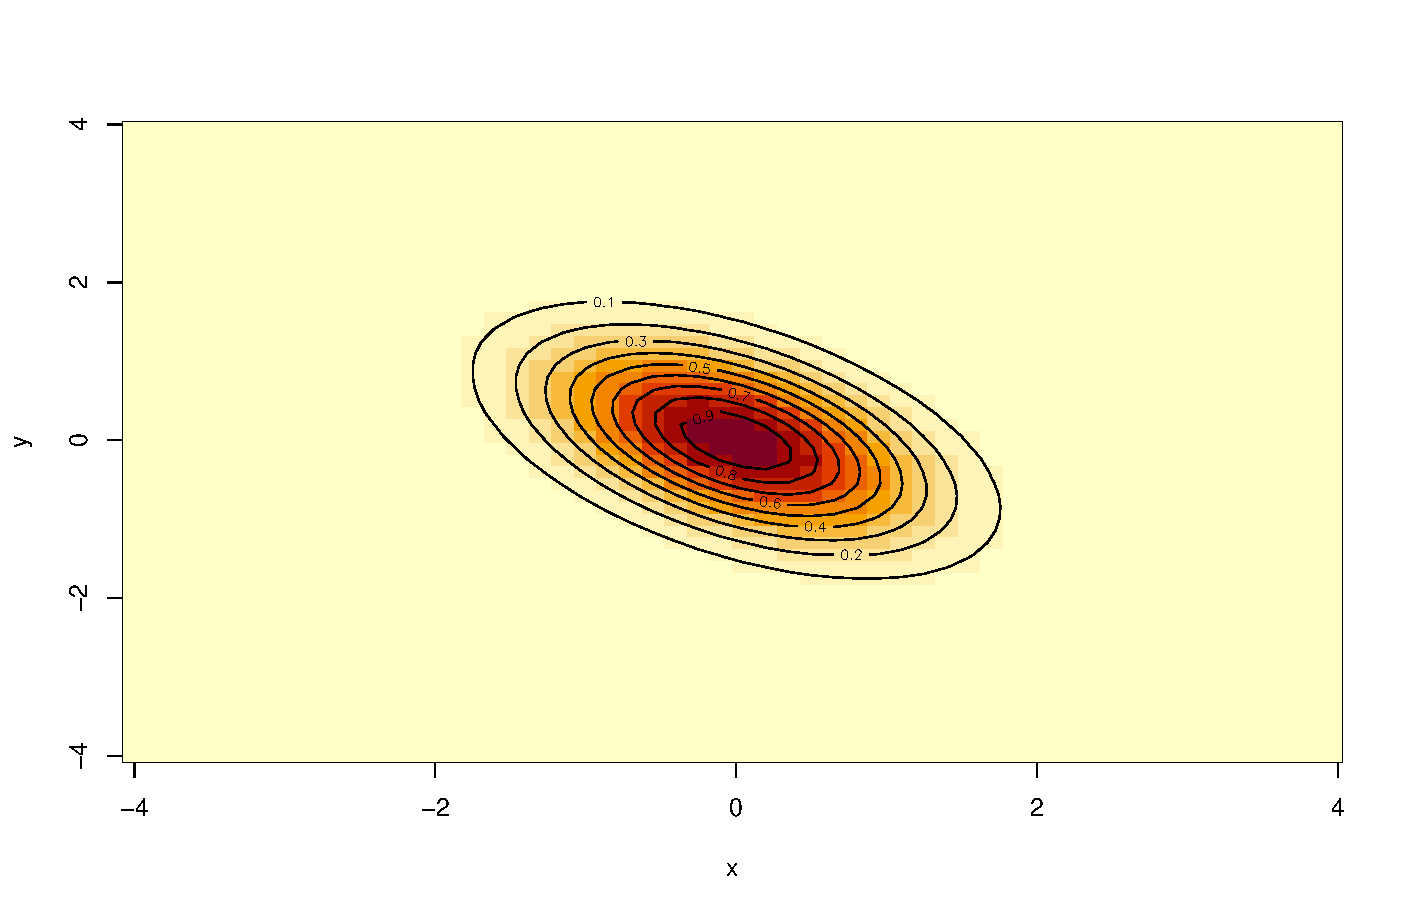
\includegraphics[width=\textwidth]{img/3d-plots-func-for-new-libs-2.pdf}
        \caption*{Image created after applying the \texttt{contour} function.}
    \end{figure}

    \newpage

    \noindent
    It's also possible to print a perspective plot using the \texttt{persp} function.
    \lstinputlisting[language=R, firstline=30, lastline=32]{code/3d-plots-func-for-new-libs-1.r}

    \begin{figure}[!htp]
        \centering
        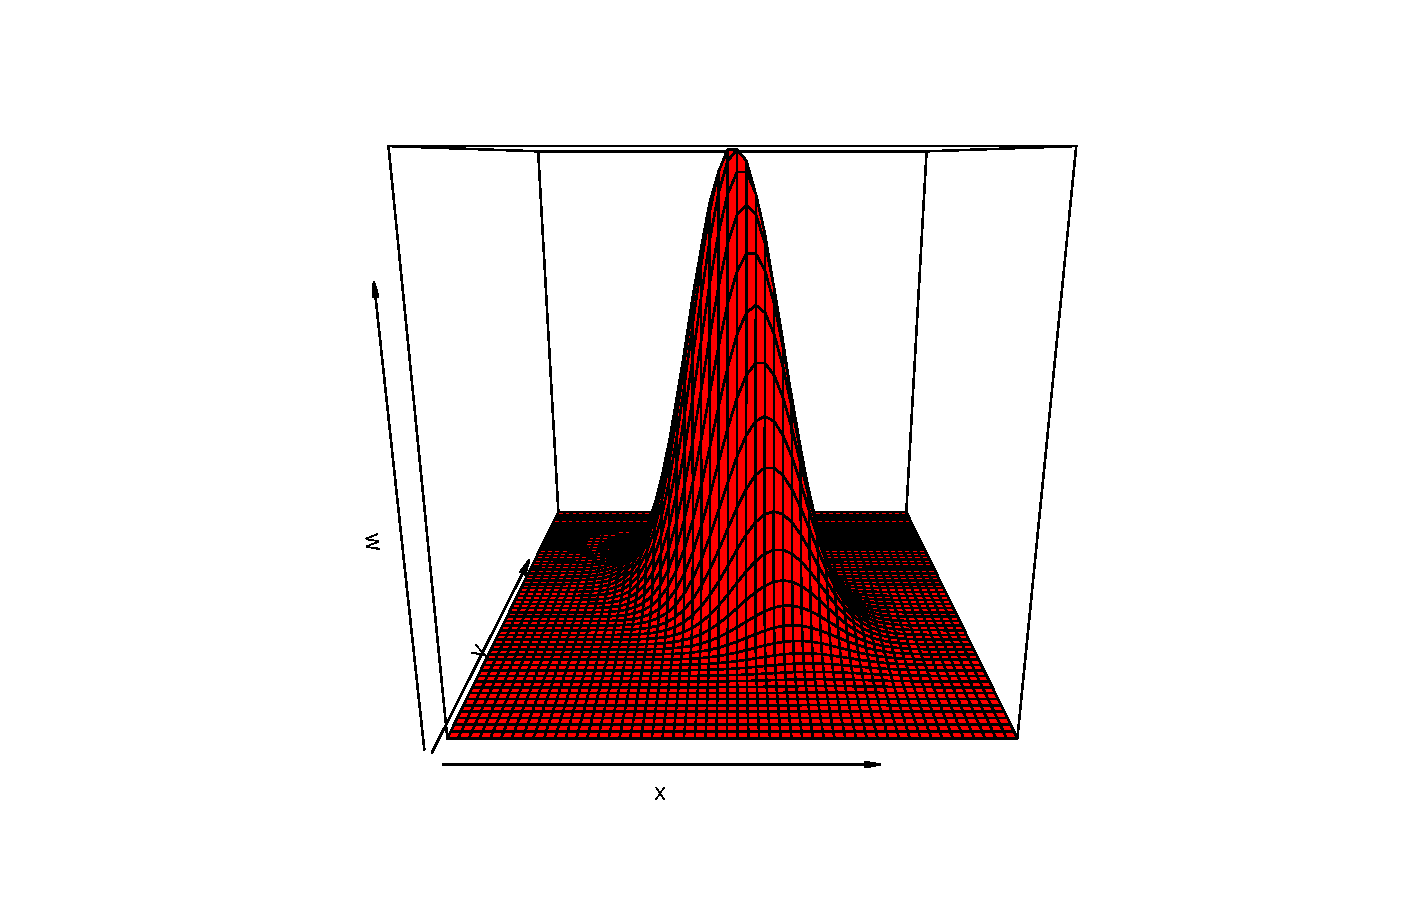
\includegraphics[width=.6\textwidth]{img/3d-plots-func-for-new-libs-3.pdf}
        \caption*{Image created with \texttt{persp} function.}
    \end{figure}

    \begin{figure}[!htp]
        \centering
        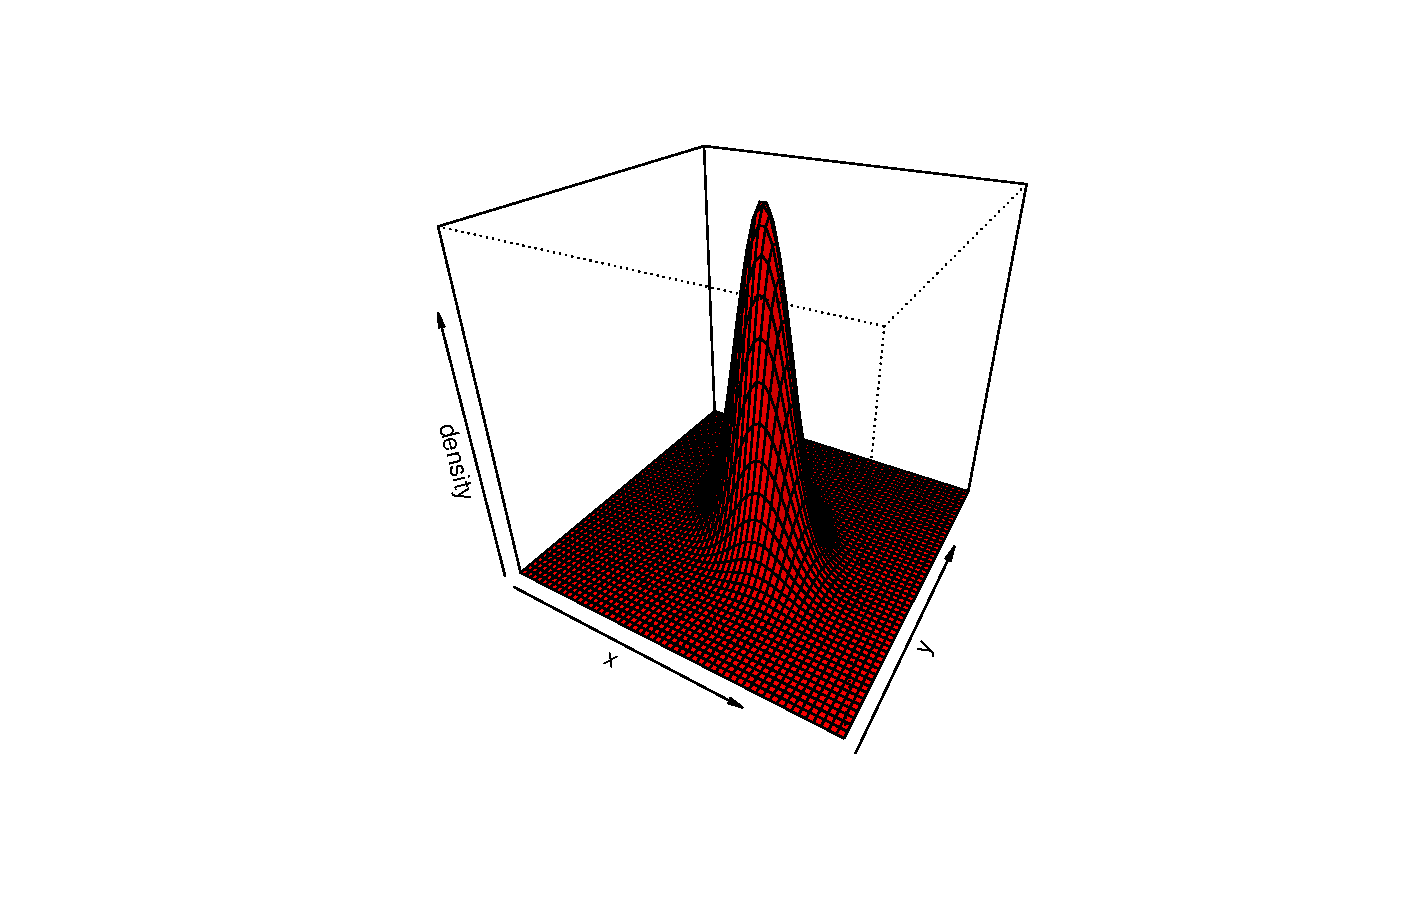
\includegraphics[width=.6\textwidth]{img/3d-plots-func-for-new-libs-4.pdf}
        \caption*{Image created after changing the perspective.}
    \end{figure}

    \newpage

    \noindent
    To get the same result but with a 3D plot, it's recommended to use the \href{https://cran.r-project.org/web/packages/rgl/index.html}{rgl library}.
    \lstinputlisting[language=R, firstline=35, lastline=52]{code/3d-plots-func-for-new-libs-1.r}
    \begin{figure}[!htp]
        \centering
        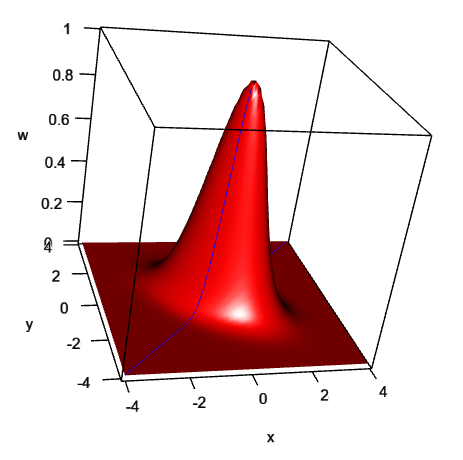
\includegraphics[width=.6\textwidth]{img/3d-plots-func-for-new-libs-5.png}
        \caption*{3D plot.}
    \end{figure}


















    %%%%%%%%%%%%%%%%%%%%%%%%%%%%%%%%%%%%%%%%%%%%%%%%%%%%%%%%%%%%%%%%%%%%%%%%%%%%%%%%%%%%%%%%
    %%%%%%%%%%%%%%%%%%%%%%%%%%%%%%%%%%%%%%%%%%%%%%%%%%%%%%%%%%%%%%%%%%%%%%%%%%%%%%%%%%%%%%%%
    %%%%%%%%%%%%%%%%%%%%%%%%%%%%%%%%%%%%%%%%%% END %%%%%%%%%%%%%%%%%%%%%%%%%%%%%%%%%%%%%%%%%
    %%%%%%%%%%%%%%%%%%%%%%%%%%%%%%%%%%%%%%%%%%%%%%%%%%%%%%%%%%%%%%%%%%%%%%%%%%%%%%%%%%%%%%%%
    %%%%%%%%%%%%%%%%%%%%%%%%%%%%%%%%%%%%%%%%%%%%%%%%%%%%%%%%%%%%%%%%%%%%%%%%%%%%%%%%%%%%%%%%


    \newpage

    \bibliography{bibtex}{}
    \bibliographystyle{plain}

    \newpage

    \printindex
\end{document}